\documentclass{article}

% ------------------------ Packages ------------------------
\usepackage{amsmath, amssymb}
\usepackage{tikz}
\usepackage{graphicx}
\usepackage{caption}
\usepackage[margin=1in]{geometry} % 전체 문서: portrait
\usepackage{pdflscape}            % 특정 페이지만 가로(landscape)로
\usetikzlibrary{shapes, arrows, positioning, fit, calc}
\usetikzlibrary{shapes.geometric, arrows.meta, positioning, calc, decorations.pathreplacing}

% Page numbering
\usepackage{fancyhdr}
\pagestyle{fancy}
\fancyhf{}
\fancyfoot[C]{\thepage}
\renewcommand{\headrulewidth}{0pt}

% ------------------------ Document ------------------------
\begin{document}

\title{Transformer Parallelism:\\
       A Visual, Dimension-Oriented Guide}
\author{}
\date{November 4, 2025}
\maketitle

\tableofcontents
\clearpage

% ==========================================================
% 1. Neural Network Basics
% ==========================================================
\section{Neural Network Basics}

In this section, we briefly introduce the core ideas of neural networks
for readers with no prior background. We cover the notion of tensors,
linear layers, activation functions, and the backpropagation algorithm
at a high level.

\subsection{What is a Neural Network?}
Here we describe the basic idea of a neural network as a composition of
linear transformations and non-linear activation functions, operating
on vector or matrix inputs.

\subsection{Fully-Connected Layers and MLPs}
We introduce the multi-layer perceptron (MLP):
\begin{itemize}
  \item Input/output shapes $[B, D]$.
  \item Linear layer $W \in \mathbb{R}^{D_{\text{in}} \times D_{\text{out}}}$,
        bias $b \in \mathbb{R}^{D_{\text{out}}}$.
  \item Activation functions such as ReLU or GELU.
\end{itemize}
This provides the foundation for understanding the Transformer MLP block.

\subsection{Backpropagation at a Glance}
We explain the key idea of backpropagation:
\begin{itemize}
  \item Gradients flowing from the loss to earlier layers.
  \item Parameter updates using optimizers such as SGD or Adam.
\end{itemize}
The detailed backward diagrams in later sections are concrete instances
of this general principle.

\clearpage

% ==========================================================
% 2. From Neural Networks to Transformers
% ==========================================================
\section{From Neural Networks to Transformers}

\subsection{Sequence Modeling Motivation}
We consider sequence modeling tasks such as natural language processing,
time series forecasting, and speech processing. In these settings the
input is not a single vector but a \emph{sequence} of tokens, each of
which is mapped to an embedding. The model must capture dependencies
both between nearby tokens and between tokens that are far apart in
the sequence.

\subsection{The Self-Attention Idea}
Transformers address sequence modeling by using self-attention instead
of explicit recurrence. At a high level:
\begin{itemize}
  \item Each token is mapped to an input embedding.
  \item Self-attention allows every position to attend to every other
        position in the same sequence.
  \item Multi-head attention (MHA) uses several attention ``heads'' in
        parallel to capture different types of relationships.
  \item A position-wise feed-forward network (MLP block) processes each
        token independently after attention.
  \item Layer normalization, residual connections, and an output
        projection tie the blocks together and produce final logits or
        predictions.
\end{itemize}

In the following sections we make these ideas concrete using
dimension-annotated diagrams of a Transformer layer and its parallel
variants.

\clearpage

\section{Gradients and Backpropagation Basics}

This section introduces the basic notions of loss functions, gradients, and backpropagation from an abstract operator point of view. In the figures later in the document we mainly show how tensors flow along edges; the detailed Jacobian matrices are not drawn explicitly. Instead, we use a compact notation for local backward operators such as $\mathrm{d}f$, which map upstream gradients on the outputs of a node to gradients on its inputs.

\subsection{Scalar Loss and Gradient Notation}

Training a Transformer model is formulated as minimizing a scalar loss function $\mathcal{L}(\theta)$ with respect to the model parameters $\theta$. For a batch of input--target pairs $(\mathbf{X}, \mathbf{Y}_{\text{targets}})$, the model produces predictions
\[
\mathbf{Y} = f_\theta(\mathbf{X}),
\]
and a scalar loss
\[
\mathcal{L} = \mathcal{L}(\mathbf{Y}, \mathbf{Y}_{\text{targets}}).
\]

We use the differential-style notation $\mathrm{d}\theta = \partial\mathcal{L}/\partial\theta$ for gradients. For example,
\[
\mathrm{d}\mathbf{X} = \frac{\partial\mathcal{L}}{\partial\mathbf{X}}, \quad
\mathrm{d}\mathbf{W} = \frac{\partial\mathcal{L}}{\partial\mathbf{W}}, \quad
\mathrm{d}\mathbf{b} = \frac{\partial\mathcal{L}}{\partial\mathbf{b}}.
\]

In the diagrams, these gradients appear as edges labeled $\mathrm{d}\mathbf{X}$, $\mathrm{d}\mathbf{W}$, etc. together with their tensor shapes such as $[B, S, D]$ or $[D, D]$.

\subsection{Single-Input Nodes and Backward Operators}

Consider a single node in a computation graph with forward computation
\[
\mathbf{y} = f(\mathbf{x}),
\]
where $\mathbf{x}$ and $\mathbf{y}$ are vectors or tensors. Let $\mathbf{J}_f(\mathbf{x})$ denote the Jacobian of $f$ at $\mathbf{x}$. If the loss $\mathcal{L}$ depends on $\mathbf{y}$, then by the chain rule
\[
\mathrm{d}\mathbf{x} = \frac{\partial\mathcal{L}}{\partial\mathbf{x}}
= \mathbf{J}_f(\mathbf{x})^T \frac{\partial\mathcal{L}}{\partial\mathbf{y}}
= \mathbf{J}_f(\mathbf{x})^T \mathrm{d}\mathbf{y}.
\]

In the figures we do not materialize the Jacobian. Instead we introduce an \textbf{abstract backward operator} $\mathrm{d}f$ and write
\[
\boxed{\mathrm{d}\mathbf{x} = \mathrm{d}f(\mathbf{x}, \mathrm{d}\mathbf{y})},
\]
with the understanding that
\[
\mathrm{d}f(\mathbf{x}, \mathrm{d}\mathbf{y}) \equiv \mathbf{J}_f(\mathbf{x})^T \mathrm{d}\mathbf{y}.
\]

\textbf{Graphical representation:}

\begin{center}
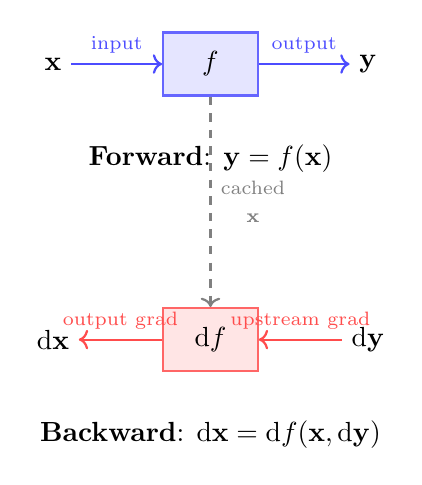
\begin{tikzpicture}[
  node distance=2cm,
  fwdnode/.style={rectangle, draw=blue!60, fill=blue!10, thick, minimum width=1.2cm, minimum height=0.8cm},
  bwdnode/.style={rectangle, draw=red!60, fill=red!10, thick, minimum width=1.2cm, minimum height=0.8cm},
  tensor/.style={},
  fwdarrow/.style={->, thick, blue!70},
  bwdarrow/.style={->, thick, red!70},
  cachearrow/.style={->, thick, dashed, gray}
]

% Forward pass
\node[tensor] (x_fwd) {$\mathbf{x}$};
\node[fwdnode, right of=x_fwd] (f_node) {$f$};
\node[tensor, right of=f_node] (y_fwd) {$\mathbf{y}$};

\draw[fwdarrow] (x_fwd) -- (f_node) node[midway, above] {\scriptsize input};
\draw[fwdarrow] (f_node) -- (y_fwd) node[midway, above] {\scriptsize output};

\node[below of=f_node, node distance=1.2cm] (fwd_label) {\textbf{Forward}: $\mathbf{y} = f(\mathbf{x})$};

% Backward pass
\node[tensor, below of=x_fwd, node distance=3.5cm] (dx_bwd) {$\mathrm{d}\mathbf{x}$};
\node[bwdnode, right of=dx_bwd] (df_node) {$\mathrm{d}f$};
\node[tensor, right of=df_node] (dy_bwd) {$\mathrm{d}\mathbf{y}$};

\draw[bwdarrow] (dy_bwd) -- (df_node) node[midway, above] {\scriptsize upstream grad};
\draw[bwdarrow] (df_node) -- (dx_bwd) node[midway, above] {\scriptsize output grad};

% Cache connection
\draw[cachearrow] (f_node) -- (df_node) node[midway, right, align=center] {\scriptsize cached\\[-2pt]\scriptsize $\mathbf{x}$};

\node[below of=df_node, node distance=1.2cm] (bwd_label) {\textbf{Backward}: $\mathrm{d}\mathbf{x} = \mathrm{d}f(\mathbf{x}, \mathrm{d}\mathbf{y})$};

\end{tikzpicture}
\end{center}

Conceptually, each backward node in the graph implements the local mapping
\[
(\mathbf{x}, \mathrm{d}\mathbf{y}) \mapsto \mathrm{d}\mathbf{x},
\]
where:
\begin{itemize}
\item \textbf{Input 1 (cached)}: The forward input $\mathbf{x}$ is cached during the forward pass
\item \textbf{Input 2 (upstream)}: The upstream gradient $\mathrm{d}\mathbf{y}$ flows from the next layer
\item \textbf{Output}: The resulting local gradient $\mathrm{d}\mathbf{x}$ flows to the previous layer
\end{itemize}

Softmax, dropout, layer normalization, and many other operators in a Transformer layer are special cases of this pattern. Their concrete backward rules are described in terms of such operators $\mathrm{d}f$.

\subsection{Nodes with Multiple Inputs}

Many nodes in a Transformer layer have several inputs. For example, a matrix multiplication node uses both an activation tensor and a weight matrix, and a layer-normalization node uses inputs as well as learned scale and shift parameters. Abstractly, we write
\[
\mathbf{y} = f(\mathbf{x}_1, \mathbf{x}_2, \ldots, \mathbf{x}_k),
\]
where each $\mathbf{x}_i$ may be a tensor of its own.

Given the upstream gradient $\mathrm{d}\mathbf{y} = \partial\mathcal{L}/\partial\mathbf{y}$, the chain rule yields gradients with respect to all inputs,
\[
\mathrm{d}\mathbf{x}_i = \mathbf{J}_{f,\mathbf{x}_i}(\mathbf{x}_1, \ldots, \mathbf{x}_k)^T \mathrm{d}\mathbf{y}, \quad i = 1, \ldots, k,
\]
where $\mathbf{J}_{f,\mathbf{x}_i}$ is the Jacobian of $f$ with respect to the $i$-th input.

We encode this in an abstract backward operator
\[
\mathrm{d}_{\mathbf{x}_i}f(\mathbf{x}_1, \ldots, \mathbf{x}_k, \mathrm{d}\mathbf{y}) := \mathbf{J}_{f,\mathbf{x}_i}(\mathbf{x}_1, \ldots, \mathbf{x}_k)^T \mathrm{d}\mathbf{y},
\]
so that, for each input,
\[
\mathrm{d}\mathbf{x}_i = \mathrm{d}_{\mathbf{x}_i}f(\mathbf{x}_1, \ldots, \mathbf{x}_k, \mathrm{d}\mathbf{y}).
\]

Collecting all input gradients together, we can also view the backward node as a single vector-valued operator
\[
\boxed{(\mathrm{d}\mathbf{x}_1, \ldots, \mathrm{d}\mathbf{x}_k) = \mathrm{d}f(\mathbf{x}_1, \ldots, \mathbf{x}_k, \mathrm{d}\mathbf{y})},
\]
whose components are exactly the individual $\mathrm{d}_{\mathbf{x}_i}f(\cdot, \ldots, \cdot, \mathrm{d}\mathbf{y})$.

\textbf{Example: Matrix Multiplication}

\begin{center}
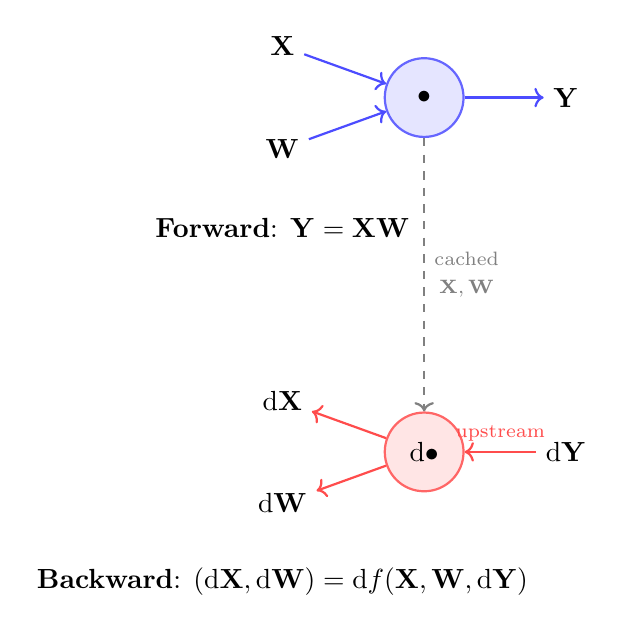
\begin{tikzpicture}[
  node distance=1.8cm,
  fwdnode/.style={circle, draw=blue!60, fill=blue!10, thick, minimum size=1cm},
  bwdnode/.style={circle, draw=red!60, fill=red!10, thick, minimum size=1cm},
  tensor/.style={},
  fwdarrow/.style={->, thick, blue!70},
  bwdarrow/.style={->, thick, red!70},
  cachearrow/.style={->, thick, dashed, gray}
]

% Forward pass
\node[tensor] (x_fwd) {$\mathbf{X}$};
\node[tensor, below of=x_fwd, node distance=1.3cm] (W_fwd) {$\mathbf{W}$};
\node[fwdnode, right of=x_fwd, yshift=-0.65cm] (f_node) {$\bullet$};
\node[tensor, right of=f_node] (y_fwd) {$\mathbf{Y}$};

\draw[fwdarrow] (x_fwd) -- (f_node);
\draw[fwdarrow] (W_fwd) -- (f_node);
\draw[fwdarrow] (f_node) -- (y_fwd);

\node[below of=W_fwd, node distance=1.0cm] (fwd_label) {\textbf{Forward}: $\mathbf{Y} = \mathbf{X}\mathbf{W}$};

% Backward pass
\node[tensor, below of=x_fwd, node distance=4.5cm] (dx_bwd) {$\mathrm{d}\mathbf{X}$};
\node[tensor, below of=W_fwd, node distance=4.5cm] (dW_bwd) {$\mathrm{d}\mathbf{W}$};
\node[bwdnode, right of=dx_bwd, yshift=-0.65cm] (df_node) {$\mathrm{d}\bullet$};
\node[tensor, right of=df_node] (dy_bwd) {$\mathrm{d}\mathbf{Y}$};

\draw[bwdarrow] (dy_bwd) -- (df_node) node[midway, above] {\scriptsize upstream};
\draw[bwdarrow] (df_node) -- (dx_bwd);
\draw[bwdarrow] (df_node) -- (dW_bwd);

% Cache connections
\draw[cachearrow] (f_node) -- (df_node) node[midway, right, align=center] {\scriptsize cached\\[-2pt]\scriptsize $\mathbf{X}, \mathbf{W}$};

\node[below of=dW_bwd, node distance=1.0cm] (bwd_label) {\textbf{Backward}: $(\mathrm{d}\mathbf{X}, \mathrm{d}\mathbf{W}) = \mathrm{d}f(\mathbf{X}, \mathbf{W}, \mathrm{d}\mathbf{Y})$};

\end{tikzpicture}
\end{center}

\vspace{0.3cm}

\noindent
\textbf{Concrete formulas:}
\begin{align*}
\mathrm{d}\mathbf{X} &= \mathrm{d}\mathbf{Y} \mathbf{W}^T \\
\mathrm{d}\mathbf{W} &= \mathbf{X}^T \mathrm{d}\mathbf{Y}
\end{align*}

In the diagrams, this is represented as a single backward node (for example, a node labeled \texttt{dMatmul} or \texttt{dLN}) with multiple incoming edges carrying the necessary forward inputs and the upstream gradient, and multiple outgoing edges carrying $\mathrm{d}\mathbf{x}_1, \ldots, \mathrm{d}\mathbf{x}_k$.

\subsection{Computation Graph and Backpropagation}

A full Transformer layer can be viewed as a composition of simpler operations:
\[
\mathbf{X}_0 \xrightarrow{f_1} \mathbf{X}_1 \xrightarrow{f_2} \mathbf{X}_2 \xrightarrow{\cdots} \mathbf{X}_L,
\]
where $\mathbf{X}_0$ is the input to the layer and $\mathbf{X}_L$ is the final output before the loss. Each $f_\ell$ is a local operator such as a matrix multiplication, a nonlinearity, a dropout, or a normalization.

Backpropagation proceeds in reverse order. Starting from $\mathrm{d}\mathbf{X}_L = \partial\mathcal{L}/\partial\mathbf{X}_L$, we apply the corresponding backward operator for each node:
\[
\mathrm{d}\mathbf{X}_\ell = \mathrm{d}f_\ell(\mathbf{X}_\ell, \mathrm{d}\mathbf{X}_{\ell+1}), \quad \ell = L-1, L-2, \ldots, 0.
\]

\textbf{Graphical representation of a computation chain:}

\begin{center}
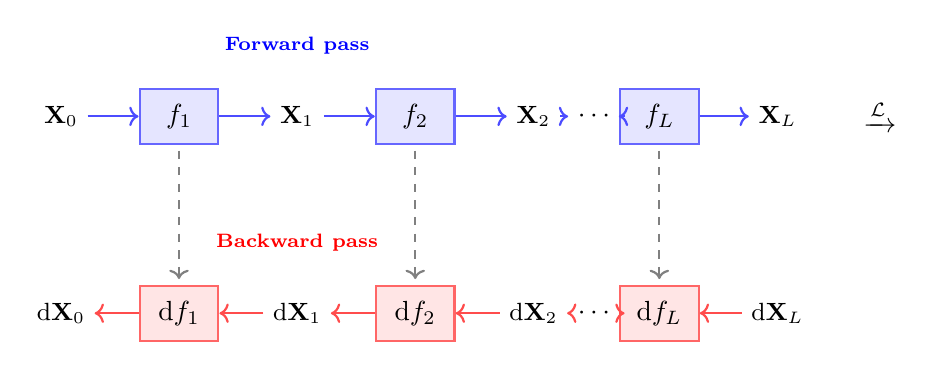
\begin{tikzpicture}[
  node distance=1.5cm,
  fwdnode/.style={rectangle, draw=blue!60, fill=blue!10, thick, minimum width=1cm, minimum height=0.7cm},
  bwdnode/.style={rectangle, draw=red!60, fill=red!10, thick, minimum width=1cm, minimum height=0.7cm},
  tensor/.style={font=\small},
  fwdarrow/.style={->, thick, blue!70},
  bwdarrow/.style={->, thick, red!70},
  cachearrow/.style={->, thick, dashed, gray, shorten >=2pt, shorten <=2pt}
]

% Forward pass
\node[tensor] (x0) {$\mathbf{X}_0$};
\node[fwdnode, right of=x0] (f1) {$f_1$};
\node[tensor, right of=f1] (x1) {$\mathbf{X}_1$};
\node[fwdnode, right of=x1] (f2) {$f_2$};
\node[tensor, right of=f2] (x2) {$\mathbf{X}_2$};
\node[right of=x2, node distance=0.8cm] (dots) {$\cdots$};
\node[fwdnode, right of=dots, node distance=0.8cm] (fL) {$f_L$};
\node[tensor, right of=fL] (xL) {$\mathbf{X}_L$};
\node[right of=xL, node distance=1.3cm] (loss) {$\xrightarrow{\mathcal{L}}$};

\draw[fwdarrow] (x0) -- (f1);
\draw[fwdarrow] (f1) -- (x1);
\draw[fwdarrow] (x1) -- (f2);
\draw[fwdarrow] (f2) -- (x2);
\draw[fwdarrow] (x2) -- (dots);
\draw[fwdarrow] (dots) -- (fL);
\draw[fwdarrow] (fL) -- (xL);

\node[above of=x1, node distance=0.9cm, blue] {\scriptsize\textbf{Forward pass}};

% Backward pass
\node[tensor, below of=x0, node distance=2.5cm] (dx0) {$\mathrm{d}\mathbf{X}_0$};
\node[bwdnode, right of=dx0] (df1) {$\mathrm{d}f_1$};
\node[tensor, right of=df1] (dx1) {$\mathrm{d}\mathbf{X}_1$};
\node[bwdnode, right of=dx1] (df2) {$\mathrm{d}f_2$};
\node[tensor, right of=df2] (dx2) {$\mathrm{d}\mathbf{X}_2$};
\node[right of=dx2, node distance=0.8cm] (bdots) {$\cdots$};
\node[bwdnode, right of=bdots, node distance=0.8cm] (dfL) {$\mathrm{d}f_L$};
\node[tensor, right of=dfL] (dxL) {$\mathrm{d}\mathbf{X}_L$};

\draw[bwdarrow] (dx1) -- (df1);
\draw[bwdarrow] (df1) -- (dx0);
\draw[bwdarrow] (dx2) -- (df2);
\draw[bwdarrow] (df2) -- (dx1);
\draw[bwdarrow] (bdots) -- (dx2);
\draw[bwdarrow] (dxL) -- (dfL);
\draw[bwdarrow] (dfL) -- (bdots);

\node[above of=dx1, node distance=0.9cm, red] {\scriptsize\textbf{Backward pass}};

% Cache arrows
\draw[cachearrow] (f1) -- (df1);
\draw[cachearrow] (f2) -- (df2);
\draw[cachearrow] (fL) -- (dfL);

\end{tikzpicture}
\end{center}

\vspace{0.3cm}

\noindent
Key observations:
\begin{itemize}
\item \textbf{Forward}: Data flows left to right through function nodes $f_\ell$
\item \textbf{Backward}: Gradients flow right to left through backward nodes $\mathrm{d}f_\ell$
\item \textbf{Cache}: Each backward node $\mathrm{d}f_\ell$ needs access to the cached forward state $\mathbf{X}_\ell$
\item \textbf{Chain rule}: $\mathrm{d}\mathbf{X}_\ell = \mathrm{d}f_\ell(\mathbf{X}_\ell, \mathrm{d}\mathbf{X}_{\ell+1})$ for $\ell = L-1, \ldots, 0$
\end{itemize}

If $f_\ell$ depends on additional inputs (e.g. parameters), then its backward operator also produces gradients with respect to those inputs, as discussed below.

In the diagrams, we emphasize this process by drawing:
\begin{itemize}
\item \textbf{forward edges} for $\mathbf{X}_\ell$ flowing into the forward nodes $f_\ell$,
\item \textbf{backward edges} for $\mathrm{d}\mathbf{X}_\ell$ flowing out of the corresponding backward nodes $\mathrm{d}f_\ell$.
\end{itemize}

The detailed formulas that define each local operator $\mathrm{d}f_\ell$ are hidden inside the node and explained in the operator dictionary of Section 4.

\subsection{Parameter Gradients and Updates}

Parameters such as weight matrices and bias vectors enter the graph as additional inputs to some node. For example, consider a matrix multiplication
\[
\mathbf{Y} = \mathbf{X}\mathbf{W},
\]
where $\mathbf{X}$ is an activation tensor and $\mathbf{W}$ is a weight matrix. We view this as a function of two inputs,
\[
\mathbf{Y} = f(\mathbf{X}, \mathbf{W}).
\]

The corresponding backward operator produces both activation and parameter gradients:
\[
\boxed{(\mathrm{d}\mathbf{X}, \mathrm{d}\mathbf{W}) = \mathrm{d}f(\mathbf{X}, \mathbf{W}, \mathrm{d}\mathbf{Y})}.
\]

\textbf{Parameter gradient flow:}

\begin{center}
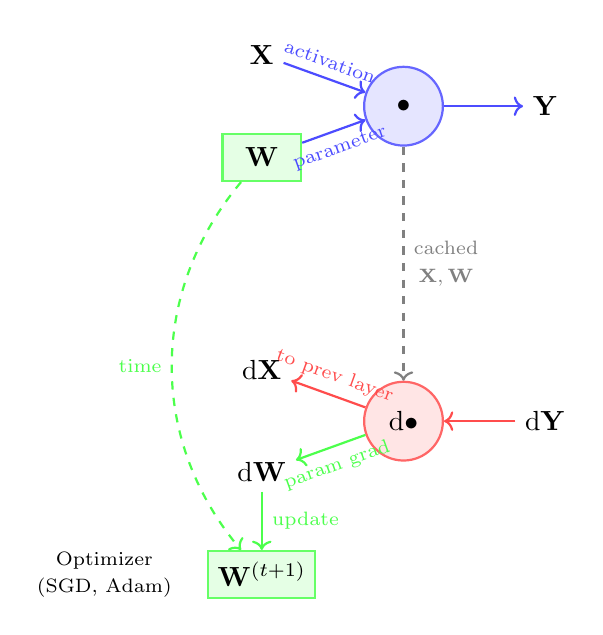
\begin{tikzpicture}[
  node distance=1.8cm,
  fwdnode/.style={circle, draw=blue!60, fill=blue!10, thick, minimum size=1cm},
  bwdnode/.style={circle, draw=red!60, fill=red!10, thick, minimum size=1cm},
  paramnode/.style={rectangle, draw=green!60, fill=green!10, thick, minimum width=1cm, minimum height=0.6cm},
  tensor/.style={},
  fwdarrow/.style={->, thick, blue!70},
  bwdarrow/.style={->, thick, red!70},
  paramarrow/.style={->, thick, green!70},
  cachearrow/.style={->, thick, dashed, gray}
]

% Forward pass
\node[tensor] (x_fwd) {$\mathbf{X}$};
\node[paramnode, below of=x_fwd, node distance=1.3cm] (W_fwd) {$\mathbf{W}$};
\node[fwdnode, right of=x_fwd, yshift=-0.65cm] (f_node) {$\bullet$};
\node[tensor, right of=f_node] (y_fwd) {$\mathbf{Y}$};

\draw[fwdarrow] (x_fwd) -- (f_node) node[midway, above, sloped] {\scriptsize activation};
\draw[fwdarrow] (W_fwd) -- (f_node) node[midway, below, sloped] {\scriptsize parameter};
\draw[fwdarrow] (f_node) -- (y_fwd);

% Backward pass
\node[tensor, below of=x_fwd, node distance=4cm] (dx_bwd) {$\mathrm{d}\mathbf{X}$};
\node[tensor, below of=W_fwd, node distance=4cm] (dW_bwd) {$\mathrm{d}\mathbf{W}$};
\node[bwdnode, right of=dx_bwd, yshift=-0.65cm] (df_node) {$\mathrm{d}\bullet$};
\node[tensor, right of=df_node] (dy_bwd) {$\mathrm{d}\mathbf{Y}$};

\draw[bwdarrow] (dy_bwd) -- (df_node);
\draw[bwdarrow] (df_node) -- (dx_bwd) node[midway, above, sloped] {\scriptsize to prev layer};
\draw[paramarrow] (df_node) -- (dW_bwd) node[midway, below, sloped] {\scriptsize param grad};

% Optimizer
\node[paramnode, below of=dW_bwd, node distance=1.3cm] (W_next) {$\mathbf{W}^{(t+1)}$};
\node[left of=W_next, node distance=2cm, align=center] (opt_label) {\scriptsize Optimizer\\[-2pt]\scriptsize (SGD, Adam)};

\draw[paramarrow] (dW_bwd) -- (W_next) node[midway, right] {\scriptsize update};
\draw[paramarrow, dashed, bend right=40] (W_fwd) to node[midway, left] {\scriptsize time} (W_next);

% Cache connections
\draw[cachearrow] (f_node) -- (df_node) node[midway, right, align=center] {\scriptsize cached\\[-2pt]\scriptsize $\mathbf{X}, \mathbf{W}$};

\end{tikzpicture}
\end{center}

\vspace{0.3cm}

\noindent
An optimizer then uses the parameter gradients to update the parameters. For example, stochastic gradient descent with learning rate $\eta$ performs
\[
\theta^{(t+1)} = \theta^{(t)} - \eta \, \mathrm{d}\theta^{(t)}.
\]

\textbf{Key distinction}:
\begin{itemize}
\item \textbf{Activation gradients} ($\mathrm{d}\mathbf{X}$): Flow to the previous layer in the backward pass
\item \textbf{Parameter gradients} ($\mathrm{d}\mathbf{W}$): Accumulated and used by the optimizer to update weights
\end{itemize}

In this document we do not draw optimizer steps in the diagrams; we only show how $\mathrm{d}\mathbf{W}$ and $\mathrm{d}\mathbf{b}$ are computed by the backward nodes.

\subsection{Connection to the Diagrams}

The detailed MHA, MLP, and output-projection figures in later sections are best read with this abstract picture in mind:
\begin{itemize}
\item Each \textbf{forward node} (e.g. \texttt{SM}, \texttt{S}, \texttt{DO}, \texttt{LN}, \texttt{matmul}) represents a mapping $\mathbf{y} = f(\mathbf{x}_1, \ldots, \mathbf{x}_k)$.
\item Each corresponding \textbf{backward node} (e.g. \texttt{dSM}, \texttt{dS}, \texttt{dDO}, \texttt{dLN}, \texttt{dMatmul}) represents the operator
\[
(\mathrm{d}\mathbf{x}_1, \ldots, \mathrm{d}\mathbf{x}_k) = \mathrm{d}f(\mathbf{x}_1, \ldots, \mathbf{x}_k, \mathrm{d}\mathbf{y}),
\]
implemented using the appropriate Jacobian-transpose formulas for that operator.
\item Edges labeled with tensors such as $\mathbf{X}$, $\mathbf{H}$, $\mathbf{Q}$, $\mathbf{K}$, $\mathbf{V}$, $\mathbf{AS}$, and their gradients $\mathrm{d}\mathbf{X}$, $\mathrm{d}\mathbf{Q}$, $\mathrm{d}\mathbf{W}$, etc., capture only the flow of data, together with compact shape annotations like $[B, S, D]$ or $[B, N_H, S, D_h]$.
\end{itemize}

In the next section we define the graphical notation and operator dictionary used in the figures, and we specialize the abstract backward operator $\mathrm{d}f$ to concrete nodes such as softmax (\texttt{S}/\texttt{dS}), scale/mask (\texttt{SM}/\texttt{dSM}), dropout (\texttt{DO}/\texttt{dDO}), and layer normalization (\texttt{LN}/\texttt{dLN}).


\section{Graphical Notation and Figure Conventions}

The diagrams in this document are designed to show how tensors flow through a Transformer layer and its parallel variants. This section summarizes the graphical notation, including tensor-shape labels, node types, edge styles, and the small operator dictionary for the most common nodes (matmul, softmax, scale/mask, dropout, layer normalization, communication, and broadcast).

Throughout the figures, the goal is to emphasize the flow of tensors along edges. The exact Jacobian matrices for each operation are not drawn; instead, the backward nodes are understood as the abstract operators $\mathrm{d}f$ introduced in Section 3.

\subsection{Tensor Shapes and Index Notation}

We use a consistent braced notation for tensor shapes. Instead of writing $\mathbb{R}^{B \times S \times D}$, we annotate edges in the diagrams with labels such as
\[
[B, S, D], \quad [B, N_H, S, D_h], \quad [D, D_{ff}],
\]
directly next to the arrows. This makes it easier to match each edge to a particular dimension ordering.

The main symbols are:
\begin{itemize}
\item $B$: batch size.
\item $S$: sequence length (number of tokens per sequence).
\item $D$: model (hidden) dimension.
\item $D_{ff}$: intermediate MLP (feed-forward) dimension.
\item $N_H$: number of attention heads.
\item $D_h$: per-head dimension, typically $D_h = D/N_H$.
\end{itemize}

Typical tensor shapes in the diagrams include:
\begin{itemize}
\item $\mathbf{X} \in [B, S, D]$: input or hidden states.
\item $\mathbf{H} \in [B, S, D]$: normalized or intermediate states.
\item $\mathbf{Q}, \mathbf{K}, \mathbf{V} \in [B, N_H, S, D_h]$: projected queries, keys, and values.
\item $\mathbf{AS} \in [B, N_H, S, S]$: attention scores after scaling/masking and softmax.
\item $\mathbf{Y} \in [B, S, D]$: output of a Transformer block or layer.
\end{itemize}

Under tensor parallelism (TP) and data parallelism (DP) we mostly keep the same shape notation on edges. For example, a TP shard that actually stores a slice of width $D/N_T$ may still be labeled $[B, S, D]$ in an end-to-end figure when we want to focus on the logical model dimension rather than the physical shard size. When necessary, shard dimensions such as $[B, S, D/N_T]$ or $[B, N_H/N_T, S, D_h]$ are written explicitly.

Gradients use the same shape conventions. For example:
\[
\mathrm{d}\mathbf{X} \in [B, S, D], \quad \mathrm{d}\mathbf{W}_Q \in [D, D], \quad \mathrm{d}\mathbf{W}_{\text{up}} \in [D, D_{ff}].
\]

\subsection{Nodes, Edges, and Arrow Styles}

The diagrams are drawn as computation graphs. Nodes represent local operations; edges represent tensors flowing between them.

\subsubsection{Forward vs. Backward Arrows}

We distinguish between forward and backward flows:
\begin{itemize}
\item \textbf{Overall flow diagrams} (e.g. the top-level Transformer flow) use:
  \begin{itemize}
  \item solid arrows for forward activations (e.g. $\mathbf{X}$ to $\mathbf{Y}$);
  \item dashed arrows for backward gradients (e.g. $\mathrm{d}\mathbf{Y}$ to $\mathrm{d}\mathbf{X}$).
  \end{itemize}
\item \textbf{Detailed backward diagrams} (e.g. MHA backward, MLP backward) use thicker arrows with different styles (single vs. double) to distinguish:
  \begin{itemize}
  \item gradient flow along the main backward path,
  \item cached forward values reused as secondary inputs to backward nodes.
  \end{itemize}
\end{itemize}

In all cases, the arrow direction follows the direction of computation for forward edges and the direction of gradient propagation for backward edges.

\subsubsection{Node Types}

We use a small set of recurring node types:

\paragraph{Matrix multiplication.} A matrix multiplication node is drawn as a circle containing a dot:
\[
\bullet
\]
In the forward pass this corresponds to an operation such as $\mathbf{Y} = \mathbf{X}\mathbf{W}$. In the backward diagrams the corresponding dNode (e.g. \texttt{dMatmul}) implements the abstract backward operator
\[
(\mathrm{d}\mathbf{X}, \mathrm{d}\mathbf{W}) = \mathrm{d}f(\mathbf{X}, \mathbf{W}, \mathrm{d}\mathbf{Y}),
\]
as described in Section 3.

\paragraph{Addition and residuals.} Elementwise addition is drawn as a circle containing a plus:
\[
+
\]
This is used for bias addition, combining residual connections, and aggregating multiple gradient contributions. Small circles labeled $\sum$ denote explicit summations over batch and/or sequence dimensions (e.g. $\sum_{B,S}$ for bias-gradient accumulation).

\paragraph{Generic rectangular operators.} Many local operations (layer normalization, nonlinearity, dropout, scale/mask, reshape, transpose) are drawn as rectangles with short labels such as \texttt{LN}, \texttt{GL}, \texttt{DO}, \texttt{SM}, \texttt{R}, or \texttt{T}. Their backward counterparts are labeled with a leading ``d'', for example \texttt{dLN}, \texttt{dDO}, \texttt{dSM}. Each such dNode implements the corresponding backward operator $\mathrm{d}f(\cdot, \ldots, \cdot, \mathrm{d}\mathbf{y})$.

\paragraph{Communication nodes.} Distributed communication collectives are drawn as small rectangular nodes with labels such as:
\begin{itemize}
\item \texttt{AR}: All-Reduce.
\item \texttt{AG}: All-Gather.
\end{itemize}
The arrows entering/leaving these nodes indicate which tensors are participating in the collective, and the shape annotations show the logical tensor size before and after the communication.

\subsection{Forward and Backward Nodes: Abstract View}

Most operators in a Transformer layer can be written abstractly as
\[
\mathbf{y} = f(\mathbf{x}_1, \ldots, \mathbf{x}_k),
\]
where $\mathbf{x}_1, \ldots, \mathbf{x}_k$ include both activations and parameters (such as weight matrices or bias vectors). In Section 3 we introduced the abstract backward operators
\[
\mathrm{d}\mathbf{x}_i = \mathrm{d}_{\mathbf{x}_i}f(\mathbf{x}_1, \ldots, \mathbf{x}_k, \mathrm{d}\mathbf{y}), \quad i = 1, \ldots, k.
\]

\textbf{How to read nodes in our diagrams:}

\begin{center}
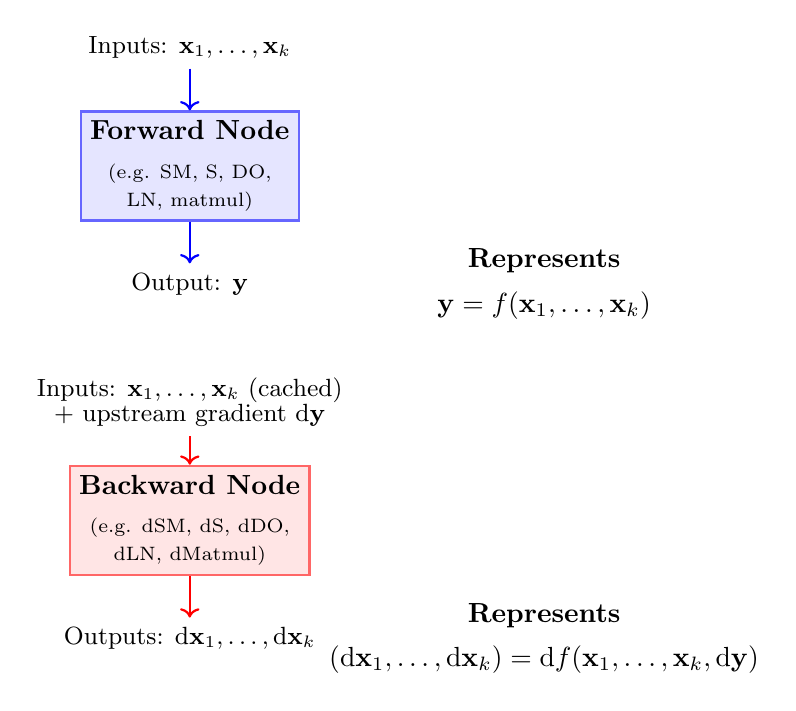
\begin{tikzpicture}[
  node distance=2.5cm,
  fwdnode/.style={rectangle, draw=blue!60, fill=blue!10, thick, minimum width=1.8cm, minimum height=1cm, align=center},
  bwdnode/.style={rectangle, draw=red!60, fill=red!10, thick, minimum width=1.8cm, minimum height=1cm, align=center},
  arrow/.style={->, thick},
  label/.style={font=\small}
]

% Forward node
\node[fwdnode] (fwd) {\textbf{Forward Node}\\[2pt]\scriptsize (e.g. SM, S, DO,\\[-2pt]\scriptsize LN, matmul)};

\node[above of=fwd, node distance=1.5cm, label] (fwd_in) {Inputs: $\mathbf{x}_1, \ldots, \mathbf{x}_k$};
\node[below of=fwd, node distance=1.5cm, label] (fwd_out) {Output: $\mathbf{y}$};

\draw[arrow, blue] (fwd_in) -- (fwd);
\draw[arrow, blue] (fwd) -- (fwd_out);

\node[right of=fwd_out, node distance=4.5cm, align=center] (fwd_eq) {
  \textbf{Represents}\\[4pt]
  $\mathbf{y} = f(\mathbf{x}_1, \ldots, \mathbf{x}_k)$
};

% Backward node
\node[bwdnode, below of=fwd, node distance=4.5cm] (bwd) {\textbf{Backward Node}\\[2pt]\scriptsize (e.g. dSM, dS, dDO,\\[-2pt]\scriptsize dLN, dMatmul)};

\node[above of=bwd, node distance=1.5cm, label, align=center] (bwd_in) {Inputs: $\mathbf{x}_1, \ldots, \mathbf{x}_k$ (cached)\\[-2pt] + upstream gradient $\mathrm{d}\mathbf{y}$};
\node[below of=bwd, node distance=1.5cm, label] (bwd_out) {Outputs: $\mathrm{d}\mathbf{x}_1, \ldots, \mathrm{d}\mathbf{x}_k$};

\draw[arrow, red] (bwd_in) -- (bwd);
\draw[arrow, red] (bwd) -- (bwd_out);

\node[right of=bwd_out, node distance=4.5cm, align=center] (bwd_eq) {
  \textbf{Represents}\\[4pt]
  $(\mathrm{d}\mathbf{x}_1, \ldots, \mathrm{d}\mathbf{x}_k) = \mathrm{d}f(\mathbf{x}_1, \ldots, \mathbf{x}_k, \mathrm{d}\mathbf{y})$
};

\end{tikzpicture}
\end{center}

\vspace{0.3cm}

In the diagrams:
\begin{itemize}
\item A \textbf{forward node} (e.g. \texttt{S}, \texttt{SM}, \texttt{DO}, \texttt{LN}, \texttt{matmul}) represents the mapping $\mathbf{y} = f(\mathbf{x}_1, \ldots, \mathbf{x}_k)$.
\item The corresponding \textbf{backward node} (labeled with a leading ``d'', e.g. \texttt{dS}, \texttt{dSM}, \texttt{dDO}, \texttt{dLN}) represents the mapping
\[
(\mathrm{d}\mathbf{x}_1, \ldots, \mathrm{d}\mathbf{x}_k) = \mathrm{d}f(\mathbf{x}_1, \ldots, \mathbf{x}_k, \mathrm{d}\mathbf{y}),
\]
i.e. it consumes the upstream gradient $\mathrm{d}\mathbf{y}$ and the necessary cached forward inputs, and produces gradients for all inputs.
\end{itemize}

The purpose of this section is not to re-derive all Jacobian formulas, but to provide a dictionary that tells the reader what each node means in the diagrams and how to read its inputs/outputs at the level of tensors and gradients.

\subsection{Operator Dictionary: Forward and Backward}

We now describe the most common node types used in the MHA, MLP, and output-projection diagrams. For each operator we briefly summarize the forward computation and the corresponding backward operator in the abstract notation $\mathrm{d}f(\cdot, \ldots, \cdot, \mathrm{d}\mathbf{y})$.

\subsubsection{Matrix Multiplication (Matmul)}

\textbf{Forward.} A matmul node computes
\[
\mathbf{Y} = \mathbf{X}\mathbf{W},
\]
with shapes such as $\mathbf{X} \in [B, S, D]$, $\mathbf{W} \in [D, D]$, and $\mathbf{Y} \in [B, S, D]$. The same pattern appears in the MLP block with $\mathbf{W}_{\text{up}} \in [D, D_{ff}]$ or $\mathbf{W}_{\text{down}} \in [D_{ff}, D]$.

\textbf{Backward.} The backward node \texttt{dMatmul} implements
\[
(\mathrm{d}\mathbf{X}, \mathrm{d}\mathbf{W}) = \mathrm{d}f(\mathbf{X}, \mathbf{W}, \mathrm{d}\mathbf{Y}),
\]
with the usual formulas
\[
\mathrm{d}\mathbf{X} = \mathrm{d}\mathbf{Y}\mathbf{W}^T, \quad \mathrm{d}\mathbf{W} = \mathbf{X}^T \mathrm{d}\mathbf{Y},
\]
applied with appropriate reshaping for batched tensors. In the diagrams, $\mathbf{X}$ and $\mathbf{W}$ (or their transposes) are supplied to the \texttt{dMatmul} node via double arrows, and outgoing arrows carry $\mathrm{d}\mathbf{X}$ and $\mathrm{d}\mathbf{W}$.

\subsubsection{Broadcast (BC)}

In many diagrams we annotate bias addition by a term such as $\text{BC}_{B,S}(\mathbf{b}_0)$, which denotes a logical broadcast of a 1-D bias vector $\mathbf{b}_0 \in [D]$ or $[D_{ff}]$ across the batch and sequence dimensions to match a tensor of shape $[B, S, D]$ or $[B, S, D_{ff}]$.

\textbf{Forward.} Conceptually,
\[
\mathbf{Y} = \mathbf{X} + \text{BC}_{B,S}(\mathbf{b}_0),
\]
where $\text{BC}_{B,S}(\mathbf{b}_0)$ is a tensor in $[B, S, D]$ obtained by repeating $\mathbf{b}_0$ over the $B$ and $S$ dimensions. In the diagrams we typically draw only the addition node and label the edge near the bias with $\text{BC}_{B,S}(\mathbf{b}_0)$ to indicate that the bias is broadcast in this way.

\textbf{Backward.} The backward contribution to $\mathrm{d}\mathbf{b}_0$ is obtained by summing $\mathrm{d}\mathbf{Y}$ over the broadcast dimensions:
\[
\mathrm{d}\mathbf{b}_0 = \sum_{b=1}^B \sum_{s=1}^S \mathrm{d}\mathbf{Y}_{b,s,:},
\]
which is represented in the diagrams by a small summation node labeled $\sum_{B,S}$. The gradient $\mathrm{d}\mathbf{X}$ simply inherits $\mathrm{d}\mathbf{Y}$, since the addition is symmetric.

\subsubsection{Scale/Mask Node (SM, dSM)}

In the attention mechanism, raw scores $\mathbf{A}$ from $\mathbf{Q}\mathbf{K}^T$ are scaled and masked before softmax. This is represented by a node labeled \texttt{SM} (scale/mask).

\textbf{Forward (SM).} Given attention scores $\mathbf{A} \in [B, N_H, S, S]$, the \texttt{SM} node computes
\[
\mathbf{Z} = \text{SM}(\mathbf{A}) = \alpha \mathbf{A} + \mathbf{M},
\]
where $\alpha = 1/\sqrt{D_h}$ is a scalar and $\mathbf{M}$ encodes the mask (e.g. large negative values at disallowed positions). The shape of $\mathbf{Z}$ matches $\mathbf{A}$. The forward pass caches the scaling factor and the mask pattern.

\textbf{Backward (dSM).} The backward node \texttt{dSM} is the abstract operator
\[
\mathrm{d}\mathbf{A} = \mathrm{d}\text{SM}(\mathbf{A}, \mathrm{d}\mathbf{Z}),
\]
with
\[
\mathrm{d}\text{SM}(\mathbf{A}, \mathrm{d}\mathbf{Z}) = \alpha \, \mathrm{d}\mathbf{Z},
\]
and no gradient is propagated into the fixed mask $\mathbf{M}$. In the diagram, $\mathbf{A}$ and $\mathrm{d}\mathbf{Z}$ enter the \texttt{dSM} node, and $\mathrm{d}\mathbf{A}$ exits as the gradient with respect to the raw attention scores.

\subsubsection{Softmax Node (S, dS)}

The node labeled \texttt{S} performs softmax over the key dimension of the attention scores.

\textbf{Forward (S).} For a fixed batch $b$, head $h$, and query position $s$, let $\mathbf{z} \in \mathbb{R}^S$ be the vector of scores over keys. Softmax produces
\[
\mathbf{p} = \text{softmax}(\mathbf{z}), \quad p_i = \frac{e^{z_i}}{\sum_j e^{z_j}}.
\]
This is applied to every $(b, h, s)$, so the overall shape $[B, N_H, S, S]$ is preserved. The forward pass typically caches $\mathbf{p}$ (or $\mathbf{z}$).

\textbf{Backward (dS).} The backward node \texttt{dS} implements the local mapping
\[
\mathrm{d}\mathbf{z} = \mathrm{d}\text{S}(\mathbf{z}, \mathrm{d}\mathbf{p}),
\]
which, in Jacobian form, is
\[
\mathrm{d}\text{S}(\mathbf{z}, \mathrm{d}\mathbf{p}) = \mathbf{J}_{\text{softmax}}(\mathbf{z})^T \mathrm{d}\mathbf{p}.
\]
In practice this is computed using the standard softmax backward formula. In the diagrams, the \texttt{dS} node has incoming edges carrying $\mathbf{p}$ (or $\mathbf{z}$) and $\mathrm{d}\mathbf{p}$, and an outgoing edge carrying $\mathrm{d}\mathbf{z}$.

\subsubsection{Nonlinearities and Dropout (GL, dGL, DO, dDO)}

Rectangular nodes labeled \texttt{GL}, \texttt{GELU}, or similar denote elementwise nonlinearities; nodes labeled \texttt{DO} denote dropout.

\textbf{Forward (GL / DO).} For a generic scalar nonlinearity $g$,
\[
\mathbf{Y} = g(\mathbf{X})
\]
is applied elementwise. For dropout we write
\[
\mathbf{Y} = \text{DO}(\mathbf{X}; \mathbf{m}) = \mathbf{m} \odot \mathbf{X},
\]
where $\mathbf{m}$ is a binary mask of the same shape as $\mathbf{X}$ and $\odot$ denotes elementwise multiplication. The mask $\mathbf{m}$ is cached in the forward pass.

\textbf{Backward (dGL / dDO).} For a generic nonlinearity, the backward node \texttt{dGL} implements
\[
\mathrm{d}\mathbf{X} = \mathrm{d}\text{GL}(\mathbf{X}, \mathrm{d}\mathbf{Y}) = \mathrm{d}\mathbf{Y} \odot g'(\mathbf{X}),
\]
using the forward input $\mathbf{X}$ from the cache.

For dropout, the backward node \texttt{dDO} implements
\[
\mathrm{d}\mathbf{X} = \mathrm{d}\text{DO}(\mathbf{X}, \mathrm{d}\mathbf{Y}) = \mathbf{m} \odot \mathrm{d}\mathbf{Y}.
\]
In the diagrams, the node labeled \texttt{dDO} consumes the upstream gradient $\mathrm{d}\mathbf{Y}$ and the cached mask $\mathbf{m}$, and produces $\mathrm{d}\mathbf{X}$.

\subsubsection{Layer Normalization (LN, dLN)}

Layer normalization nodes are labeled \texttt{LN} in the forward pass and \texttt{dLN} in the backward pass.

\textbf{Forward (LN).} Given $\mathbf{X} \in [B, S, D]$, layer normalization computes
\[
\mathbf{H} = \text{LN}(\mathbf{X}; \gamma, \beta),
\]
by normalizing each $[D]$-dimensional vector at fixed $B, S$, and applying learned scale and shift parameters $\gamma, \beta \in [D]$. The forward pass caches per-position mean/variance as well as $\gamma$ and $\beta$.

\textbf{Backward (dLN).} The backward node \texttt{dLN} implements
\[
(\mathrm{d}\mathbf{X}, \mathrm{d}\gamma, \mathrm{d}\beta) = \mathrm{d}\text{LN}(\mathbf{X}, \gamma, \beta, \mathrm{d}\mathbf{H}, \text{stats}),
\]
where $\text{stats}$ denotes the cached means and variances. The explicit formulas follow from the standard layer-normalization backward derivation; in the diagrams we treat \texttt{dLN} as a single node that consumes $\mathbf{X}$, $\gamma$, the cached statistics, and $\mathrm{d}\mathbf{H}$, and produces three outgoing gradient edges $\mathrm{d}\mathbf{X}$, $\mathrm{d}\gamma$, and $\mathrm{d}\beta$.

\subsubsection{Communication Nodes (AR, AG)}

In tensor-parallel (TP), data-parallel (DP), and hybrid DP+TP settings, collective communication operations synchronize tensors across devices.

\textbf{All-Reduce (AR).} An All-Reduce node \texttt{AR} takes as input a tensor shard from each participant and outputs the elementwise reduced tensor (typically a sum), optionally divided by the number of participants for averaging. For example, in DP, weight gradients $\mathrm{d}\mathbf{W}$ of shape $[D, D]$ are All-Reduced across all data-parallel ranks before the optimizer step.

\textbf{All-Gather (AG).} An All-Gather node \texttt{AG} concatenates or aggregates tensor shards across a parallel group to reconstruct a full tensor. For example, in TP, partial outputs along a hidden dimension may be gathered to form a full $[B, S, D]$ tensor.

In the diagrams, these communication nodes are treated as pure operators on tensors; their backward behavior (e.g. gradient flow through \texttt{AR} and \texttt{AG}) is implicit in the symmetry of the operations.

\subsection{Reading the Detailed MHA and MLP Figures}

With the conventions above, the large MHA and MLP forward/backward figures can be read as follows:
\begin{itemize}
\item \textbf{Edges} indicate the flow of tensors (activations or gradients), annotated with shapes like $[B, S, D]$ or $[B, N_H, S, D_h]$.
\item \textbf{Forward nodes} (\texttt{S}, \texttt{SM}, \texttt{DO}, \texttt{LN}, \texttt{matmul}, \texttt{reshape}, \texttt{transpose}) compute local functions $f(\mathbf{x}_1, \ldots, \mathbf{x}_k)$.
\item \textbf{Backward nodes} (\texttt{dS}, \texttt{dSM}, \texttt{dDO}, \texttt{dLN}, \texttt{dMatmul}) implement the corresponding backward operators $\mathrm{d}f(\mathbf{x}_1, \ldots, \mathbf{x}_k, \mathrm{d}\mathbf{y})$, producing gradients for all inputs.
\item \textbf{Broadcast labels} such as $\text{BC}_{B,S}(\mathbf{b}_0)$ indicate that a bias vector is conceptually expanded to match a higher-rank tensor before addition.
\item \textbf{Communication nodes} (\texttt{AR}, \texttt{AG}) indicate where collective operations occur in TP, DP, or DP+TP settings, and their shape annotations show the logical dimensions involved.
\end{itemize}

These conventions allow the reader to understand the data and gradient flows at a glance, without being distracted by low-level indexing, while still being precise enough to derive the underlying equations when needed.


% ==========================================================
% 4. Single-Node Transformer: Forward and Backward
% ==========================================================
\section{Single-Node Transformer: Forward and Backward}

This section presents the full Transformer layer running on a single node
(no parallelism). We emphasize tensor shapes and data flow for both
forward and backward passes.

\subsection{Overall Transformer Layer Flow}
\resizebox{\linewidth}{!}{%
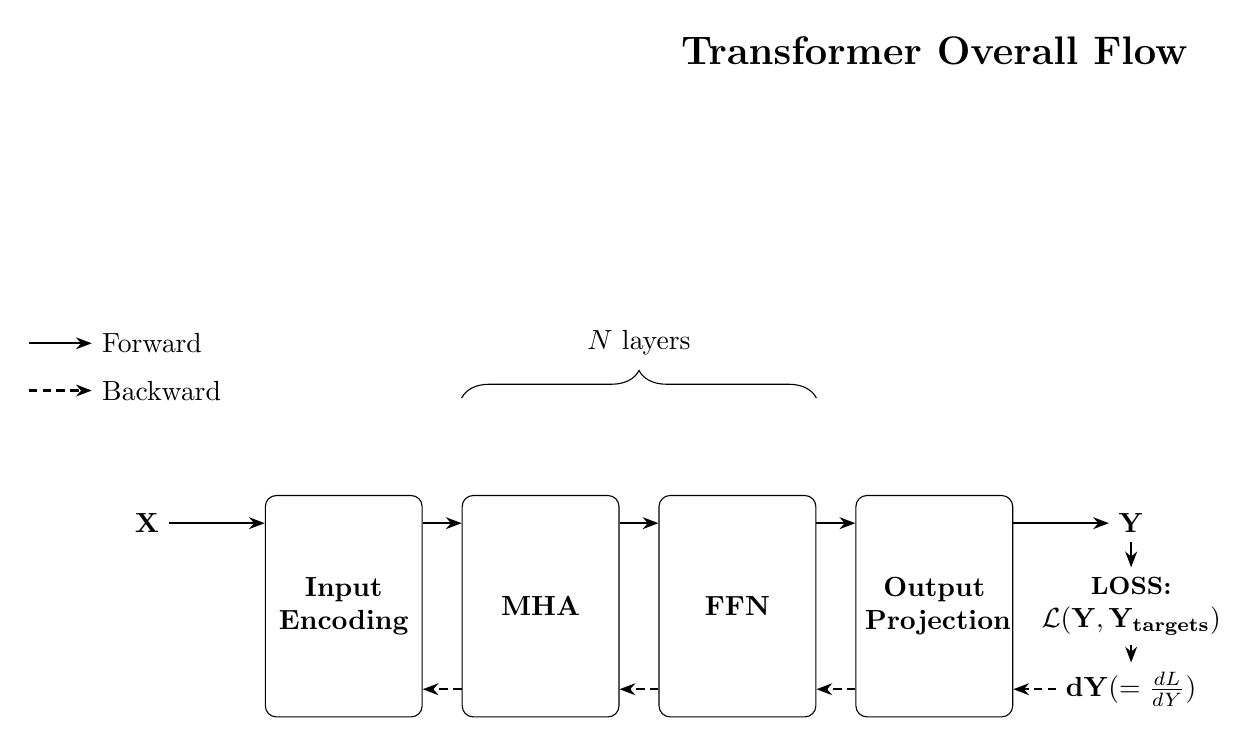
\begin{tikzpicture}[
    node distance=2.5cm,
    >=stealth,
    block/.style={rectangle, draw=black, fill=white, text width=5em, text centered, rounded corners, minimum height=8em, font=\bfseries},
    forward/.style={-{Stealth[length=2mm]}, thick, black},
    backward/.style={-{Stealth[length=2mm]}, thick, black, densely dashed},
    io/.style={text centered, font=\bfseries}
]
    % Title
    \node[font=\Large\bfseries] at (10, 6) {Transformer Overall Flow};

    % Forward path nodes (horizontal)
    \node (input) [io] {$\mathbf{X}$};
    \node (encoding) [block, right of=input, yshift=-3em] {Input\\Encoding};
    \node (mha) [block, right of=encoding] {MHA};
    \node (mlp) [block, right of=mha] {FFN};
    \node (output) [block, right of=mlp] {Output\\Projection};
    \node (pred) [io, right of=output, yshift=3em] {$\mathbf{Y}$};
    \node (loss) [align=center, io, right of=output] {\small LOSS:\\$\mathcal{L}(\mathbf{Y,Y_\text{targets}})$};
    \node (gradient) [io, right of=output, yshift=-3em] {$\mathbf{dY}(=\frac{dL}{dY})$};

    % Forward arrows (upper part of blocks)
    \draw [forward] (input) -- ([yshift=3em]encoding.west);
    \draw [forward] ([yshift=3em]encoding.east) -- ([yshift=3em]mha.west);
    \draw [forward] ([yshift=3em]mha.east) -- ([yshift=3em]mlp.west);
    \draw [forward] ([yshift=3em]mlp.east) -- ([yshift=3em]output.west);
    \draw [forward] ([yshift=3em]output.east) -- (pred);
    \draw [forward] (pred) -- (loss);
    \draw [backward] (loss) -- (gradient);

    % Backward arrows (lower part of blocks)
    \draw [backward] (gradient) -- ([yshift=-3em]output.east);
    \draw [backward] ([yshift=-3em]output.west) -- ([yshift=-3em]mlp.east);
    \draw [backward] ([yshift=-3em]mlp.west) -- ([yshift=-3em]mha.east);
    \draw [backward] ([yshift=-3em]mha.west) -- ([yshift=-3em]encoding.east);

    % Brace for layer repetition
    \draw[decorate, decoration={brace, amplitude=10pt}]
        ([yshift=3.5em]mha.north west) -- ([yshift=3.5em]mlp.north east)
        node[midway, above=12pt, font=\normalsize] {$N$ layers};

    % Labels (Legend)
    \coordinate (legend) at ([xshift=-1.5cm, yshift=6.5em]input);
    \draw[forward] (legend) -- ++(0.8,0) node[right, font=\normalsize] {Forward};
    \draw[backward] ([yshift=-0.6cm]legend) -- ++(0.8,0) node[right, font=\normalsize] {Backward};

\end{tikzpicture}%
}

\clearpage

% ------------------------ 4.1 Input Embedding ------------------------
\subsection{Input Embedding Layer}

\subsubsection{Forward Pass}
\documentclass{article}

\usepackage{amsmath, amssymb}
\usepackage{tikz}
\usepackage{graphicx}
\usepackage{caption}
\usepackage[margin=1in, landscape]{geometry}
\usetikzlibrary{shapes, arrows, positioning, fit, calc}

\begin{document}

% ---------- Input Embedding -> (to MHA) ----------
\noindent
\resizebox{\linewidth}{!}{%
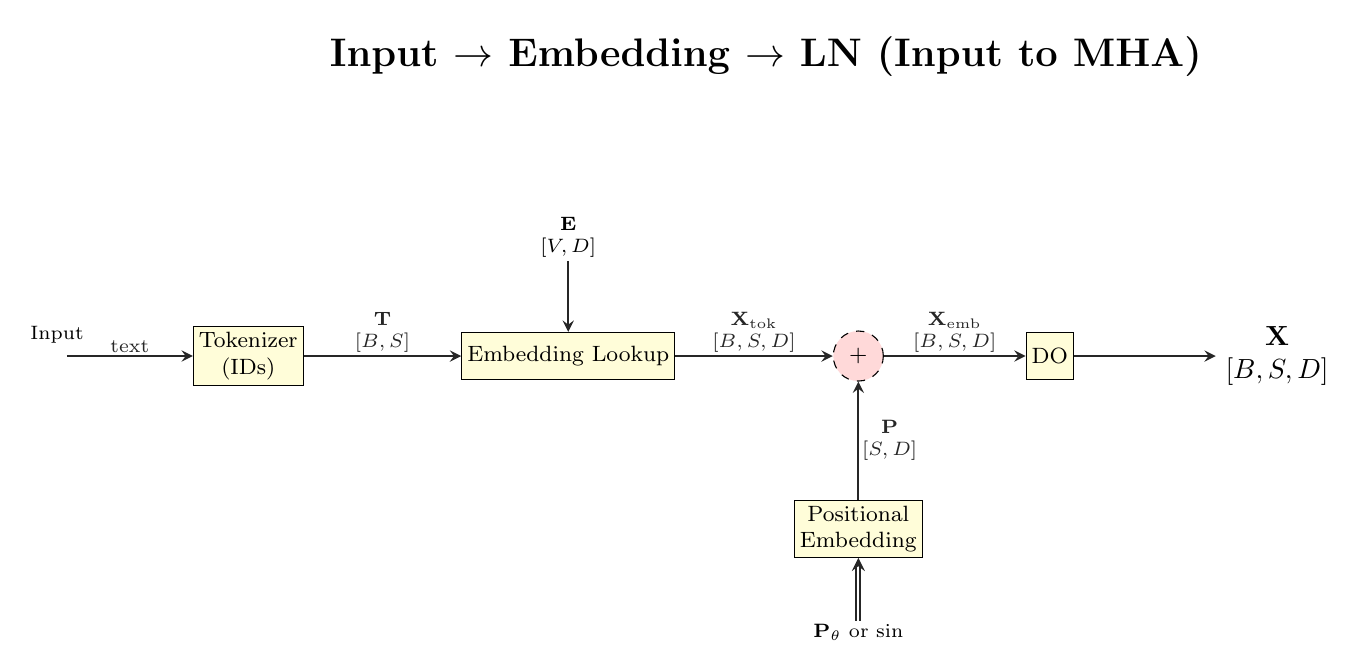
\begin{tikzpicture}[
  >=stealth,
  auxnode/.style={draw, rectangle, fill=yellow!15, minimum height=6mm, inner sep=2pt, font=\footnotesize, align=center},
  mulnode/.style={draw, circle, fill=green!15, minimum size=6mm, font=\footnotesize, align=center},
  addnode/.style={draw, circle, dashed, fill=red!15, minimum size=6mm, font=\footnotesize, align=center},
  flow/.style={->, thick, black!85},
  flow2/.style={->, double, thick, black!85},
  dimlabel/.style={font=\scriptsize, inner sep=1pt, align=center}
]

\node[font=\Large\bfseries] at (9, 3.8) {Input $\rightarrow$ Embedding $\rightarrow$ LN (Input to MHA)};

% nodes
\node (RawText) at (0,0) {};
\node[auxnode, align=center] (Tok)   [right=1.6cm of RawText] {Tokenizer\\(IDs)};
\node[auxnode, align=center] (Lookup)[right=2.0cm of Tok]     {Embedding Lookup};
\node[addnode, minimum size=6mm] (Sum) [right=2.0cm of Lookup] {+};
\node[auxnode, align=center] (PosE)  [below=1.5cm of Sum]  {Positional\\Embedding};
\node[auxnode] (Drop) [right=1.8cm of Sum] {DO};
\node (OUTPUT)   [align=center, right=1.8cm of Drop]   {$\mathbf{X}$\\$[B,S,D]$};

% parameter/const “double” edges
\node[dimlabel] (Eparam) [align=center, above=0.9cm of Lookup] {$\mathbf{E}$\\$[V,D]$};
\node[dimlabel] (Pparam) [align=center, below=0.8cm of PosE]   {$\mathbf{P}_{\theta}$ or sin};

% flows
\draw[flow] (RawText) -- (Tok) node[dimlabel, midway, above]
  {$\text{text}$};
\draw[flow] (Tok) -- (Lookup) node[dimlabel, midway, above]
  {$\mathbf{T}$\\$[B,S]$};

% Embedding matrix E
\draw[flow] (Eparam) -- (Lookup);

% Lookup -> Sum (token embeddings)
\draw[flow] (Lookup) -- (Sum) node[dimlabel, midway, above]
  {$\mathbf{X}_{\text{tok}}$\\$[B,S,D]$};

% Positional embedding path
\draw[flow] (PosE) -- (Sum) node[dimlabel, midway, right]
  {$\mathbf{P}$\\$[S,D]$};

% Optional: show P as parameter (sinusoidal/learned)
\draw[flow2] (Pparam) -- (PosE) ;

\draw[flow] (Sum) -- (Drop) node[dimlabel, midway, above]
  {$\mathbf{X}_{\text{emb}}$\\$[B,S,D]$};
\draw[flow] (Drop) -- (OUTPUT);

% labels for start and destination
\node[dimlabel, above=0.0cm of RawText] {Input};

\end{tikzpicture}%
}

\newpage
\renewcommand{\arraystretch}{1.2}
\small

% -------- Operations (Ops) --------
\begin{center}
\textbf{Operations (Ops)}
\begin{tabular}{llll}
\hline
\textbf{Abbrev} & \textbf{Name} & \textbf{Type / Shape} & \textbf{Notes} \\
\hline
Tokenizer & Tokenizer (IDs) & op & Maps raw text $\to$ integer ids $\mathbf{T}\in\mathbb{Z}^{[B,S]}$. \\
Embedding Lookup & Embedding Lookup & op & Gathers rows from $\mathbf{E}\in\mathbb{R}^{V\times D}$ using ids $\mathbf{T}$. \\
$+$ & Element-wise Add (dashed circle) & op & Adds token and positional embeddings; broadcasting over $B,S$ if needed. \\
DO & Dropout & op & Training-time stochastic dropout on $\mathbf{X}_{\text{emb}}$; identity at inference. \\
\textit{(none)} & Broadcast $\mathrm{BC}_{B,S}(\cdot)$ & op & Expands $[S,D]$ (or $[D]$) to $[B,S,D]$ across batch/sequence. \\
\hline
\end{tabular}
\end{center}

\vspace{0.8em}

% -------- Data Tensors (Values) --------
\begin{center}
\textbf{Data Tensors (Values)}
\begin{tabular}{llll}
\hline
\textbf{Symbol} & \textbf{Name} & \textbf{Shape} & \textbf{Notes} \\
\hline
text & Raw input text & — & Character/byte stream before tokenization. \\
$\mathbf{T}$ & Token ids & $[B,S]$ & Output of Tokenizer; integers in $\{0,\dots,V{-}1\}$. \\
$\mathbf{E}$ & Embedding matrix (params) & $[V,D]$ & Trainable; each vocab entry has a $D$-dim vector. \\
$\mathbf{X}_{\text{tok}}$ & Token embeddings & $[B,S,D]$ & $\mathrm{lookup}(\mathbf{E}, \mathbf{T})$. \\
$\mathbf{P}$ & Positional embedding & $[S,D]$ (or $[B,S,D]$) & Learned $\mathbf{P}_\theta$ \textbf{or} sinusoidal (fixed); broadcast to $[B,S,D]$. \\
$\mathbf{X}_{\text{emb}}$ & Sum of token+pos & $[B,S,D]$ & $\mathbf{X}_{\text{tok}} + \mathrm{BC}_{B,S}(\mathbf{P})$. \\
$\mathbf{X}$ & Input to MHA & $[B,S,D]$ & After dropout (DO); goes to LN/MHA stack. \\
$\mathbf{P}_\theta$ & Learned pos. params & matches $\mathbf{P}$ & Used when positions are trainable; otherwise “sin” denotes fixed sinusoidal. \\
\hline
\multicolumn{4}{l}{\textbf{Shape symbols:}\; $B$=batch size,\; $S$=sequence length,\; $D$=model dim,\; $V$=vocab size.} \\
\multicolumn{4}{l}{\textbf{Notes:}\; In practice, $\mathbf{P}$ may be pre-broadcast to $[B,S,D]$ or added per-token with implicit broadcasting.} \\
\hline
\end{tabular}
\end{center}

\end{document}


\clearpage

\clearpage

% ------------------------ 4.2 Multi-Head Attention -------------------
\subsection{Multi-Head Attention (MHA)}

Multi-Head Attention enables the model to jointly attend to information
from different representation subspaces.

\subsubsection{Forward Pass}

\begin{landscape}
\thispagestyle{fancy}
\resizebox{\linewidth}{!}{%
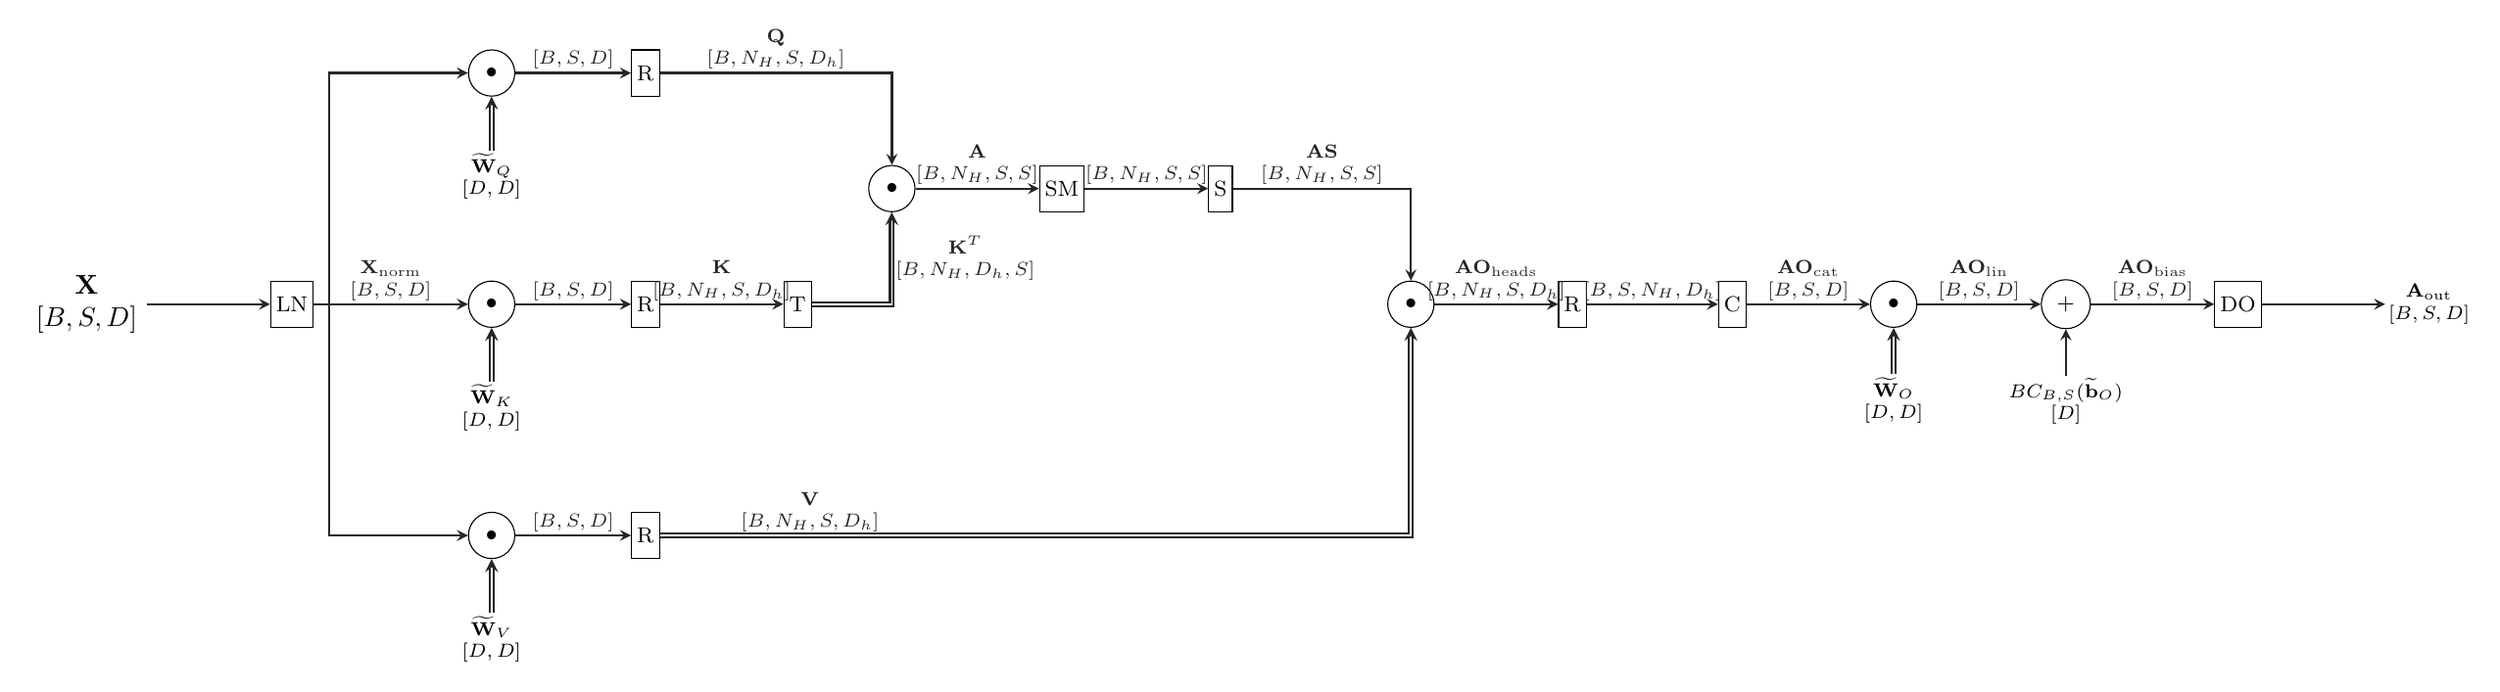
\begin{tikzpicture}[
  every node/.style={transform shape},
  >=stealth,
  auxnode/.style={draw, rectangle, fill=white, minimum height=6mm, inner sep=2pt, font=\footnotesize, align=center},
  mulnode/.style={draw, circle, fill=white, minimum size=6mm, font=\footnotesize, align=center},
  addnode/.style={draw, circle, fill=white, minimum size=6mm, font=\footnotesize, align=center},
  flow/.style={->, thick, black!85},
  flow2/.style={->, double, thick, black!85},
  dimlabel/.style={font=\scriptsize, inner sep=1pt, align=center}
]
% \node[font=\Large\bfseries] at (8, 4.5) {Multi-Head Attention Forward Pass};

\node (Input) at (0.5, 0) [align=center] {$\mathbf{X}$\\$[B,S,D]$};
\node[auxnode] (LN) [right=1.6cm of Input] {LN};

\node[mulnode] (Proj_Q) [right=2.0cm of LN, yshift=3.0cm] {$\bullet$};
\node[auxnode] (R_Q) [right=1.5cm of Proj_Q] {R};

\node[mulnode] (Proj_K) [right=2.0cm of LN, yshift=0cm] {$\bullet$};
\node[auxnode] (R_K) [right=1.5cm of Proj_K] {R};

\node[mulnode] (Proj_V) [right=2.0cm of LN, yshift=-3.0cm] {$\bullet$};
\node[auxnode] (R_V) [right=1.5cm of Proj_V] {R};

\node[dimlabel] (WQ) [align=center, below=0.7cm of Proj_Q] {$\widetilde{\mathbf{W}}_{Q}$\\$[D,D]$};
\node[dimlabel] (WK) [align=center, below=0.7cm of Proj_K] {$\widetilde{\mathbf{W}}_{K}$\\$[D,D]$};
\node[dimlabel] (WV) [align=center, below=0.7cm of Proj_V] {$\widetilde{\mathbf{W}}_{V}$\\$[D,D]$};

\node[auxnode] (T_K) [right=1.6cm of R_K] {T};
\node[mulnode] (QK) [right=2.7cm of R_Q, yshift=-1.5cm] {$\bullet$};
\node[auxnode] (SM) [right=1.6cm of QK] {SM};
\node[auxnode] (Soft) [right=1.6cm of SM] {S};
\node[mulnode] (PV) [right=2.0cm of Soft, yshift=-1.5cm] {$\bullet$};

\node[auxnode] (R_Merge) [right=1.6cm of PV] {R};
\node[auxnode] (Cat) [right=1.7cm of R_Merge] {C};

\node[mulnode] (OProj) [right=1.6cm of Cat] {$\bullet$};
\node[dimlabel] (WO_FWD) [align=center, below=0.6cm of OProj] {$\widetilde{\mathbf{W}}_{O}$\\$[D,D]$};
\node[addnode] (AddB) [right=1.6cm of OProj] {+};
\node[dimlabel] (BO) [align=center, below=0.6cm of AddB] {$BC_{B,S}(\widetilde{\mathbf{b}}_{O})$\\$[D]$};
\node[auxnode] (Drop) [right=1.6cm of AddB] {DO};
\node[dimlabel] (Aout) [align=center, right=1.6cm of Drop] {$\mathbf{A}_{\text{out}}$\\$[B,S,D]$};

\draw[flow] (Input) -- (LN);

\draw[flow] (LN.east) -- ++(0.2,0) |- (Proj_Q.west);
\draw[flow] (LN) -- (Proj_K.west) node[dimlabel, midway, above]{$\mathbf{X}_{\text{norm}}$\\$[B,S,D]$};
\draw[flow] (LN.east) -- ++(0.2,0) |- (Proj_V.west);

\draw[flow2] (WQ) -- (Proj_Q);
\draw[flow2] (WK) -- (Proj_K);
\draw[flow2] (WV) -- (Proj_V);

\draw[flow] (Proj_Q) -- (R_Q) node[dimlabel, midway, above]{$[B,S,D]$};
\draw[flow] (Proj_K) -- (R_K) node[dimlabel, midway, above]{$[B,S,D]$};
\draw[flow] (Proj_V) -- (R_V) node[dimlabel, midway, above]{$[B,S,D]$};

\draw[flow] (R_Q) -| (QK) node[dimlabel, near start, above]{$\mathbf{Q}$\\$[B,N_H,S,D_h]$};
\draw[flow] (R_K) -- (T_K) node[dimlabel, midway, above]{$\mathbf{K}$\\$[B,N_H,S,D_h]$};
\draw[flow2] (T_K) -| (QK) node[dimlabel, near end, right]{$\mathbf{K}^{T}$\\$[B,N_H,D_h,S]$};

\draw[flow] (QK) -- (SM) node[dimlabel, midway, above]{$\mathbf{A}$\\$[B,N_H,S,S]$};
\draw[flow] (SM) -- (Soft) node[dimlabel, midway, above]{$[B,N_H,S,S]$};
\draw[flow] (Soft) -| (PV) node[dimlabel, near start, above]{$\mathbf{AS}$\\$[B,N_H,S,S]$};
\draw[flow2] (R_V) -| (PV) node[dimlabel, pos=0.1, above]{$\mathbf{V}$\\$[B,N_H,S,D_h]$};

\draw[flow] (PV) -- (R_Merge) node[dimlabel, midway, above]{$\mathbf{AO}_{\text{heads}}$\\$[B,N_H,S,D_h]$};
\draw[flow] (R_Merge) -- (Cat) node[dimlabel, midway, above]{$[B,S,N_H,D_h]$};
\draw[flow] (Cat) -- (OProj) node[dimlabel, midway, above]{$\mathbf{AO}_{\text{cat}}$\\$[B,S,D]$};
\draw[flow2] (WO_FWD) -- (OProj);
\draw[flow] (OProj) -- (AddB) node[dimlabel, midway, above]{$\mathbf{AO}_{\text{lin}}$\\$[B,S,D]$};
\draw[flow] (BO) -- (AddB);
\draw[flow] (AddB) -- (Drop) node[dimlabel, midway, above]{$\mathbf{AO}_{\text{bias}}$\\$[B,S,D]$};
\draw[flow] (Drop) -- (Aout);
\end{tikzpicture}%
}

\end{landscape}
\clearpage

\subsubsection{Backward Pass}

\begin{landscape}
\thispagestyle{fancy}
\resizebox{\linewidth}{!}{%
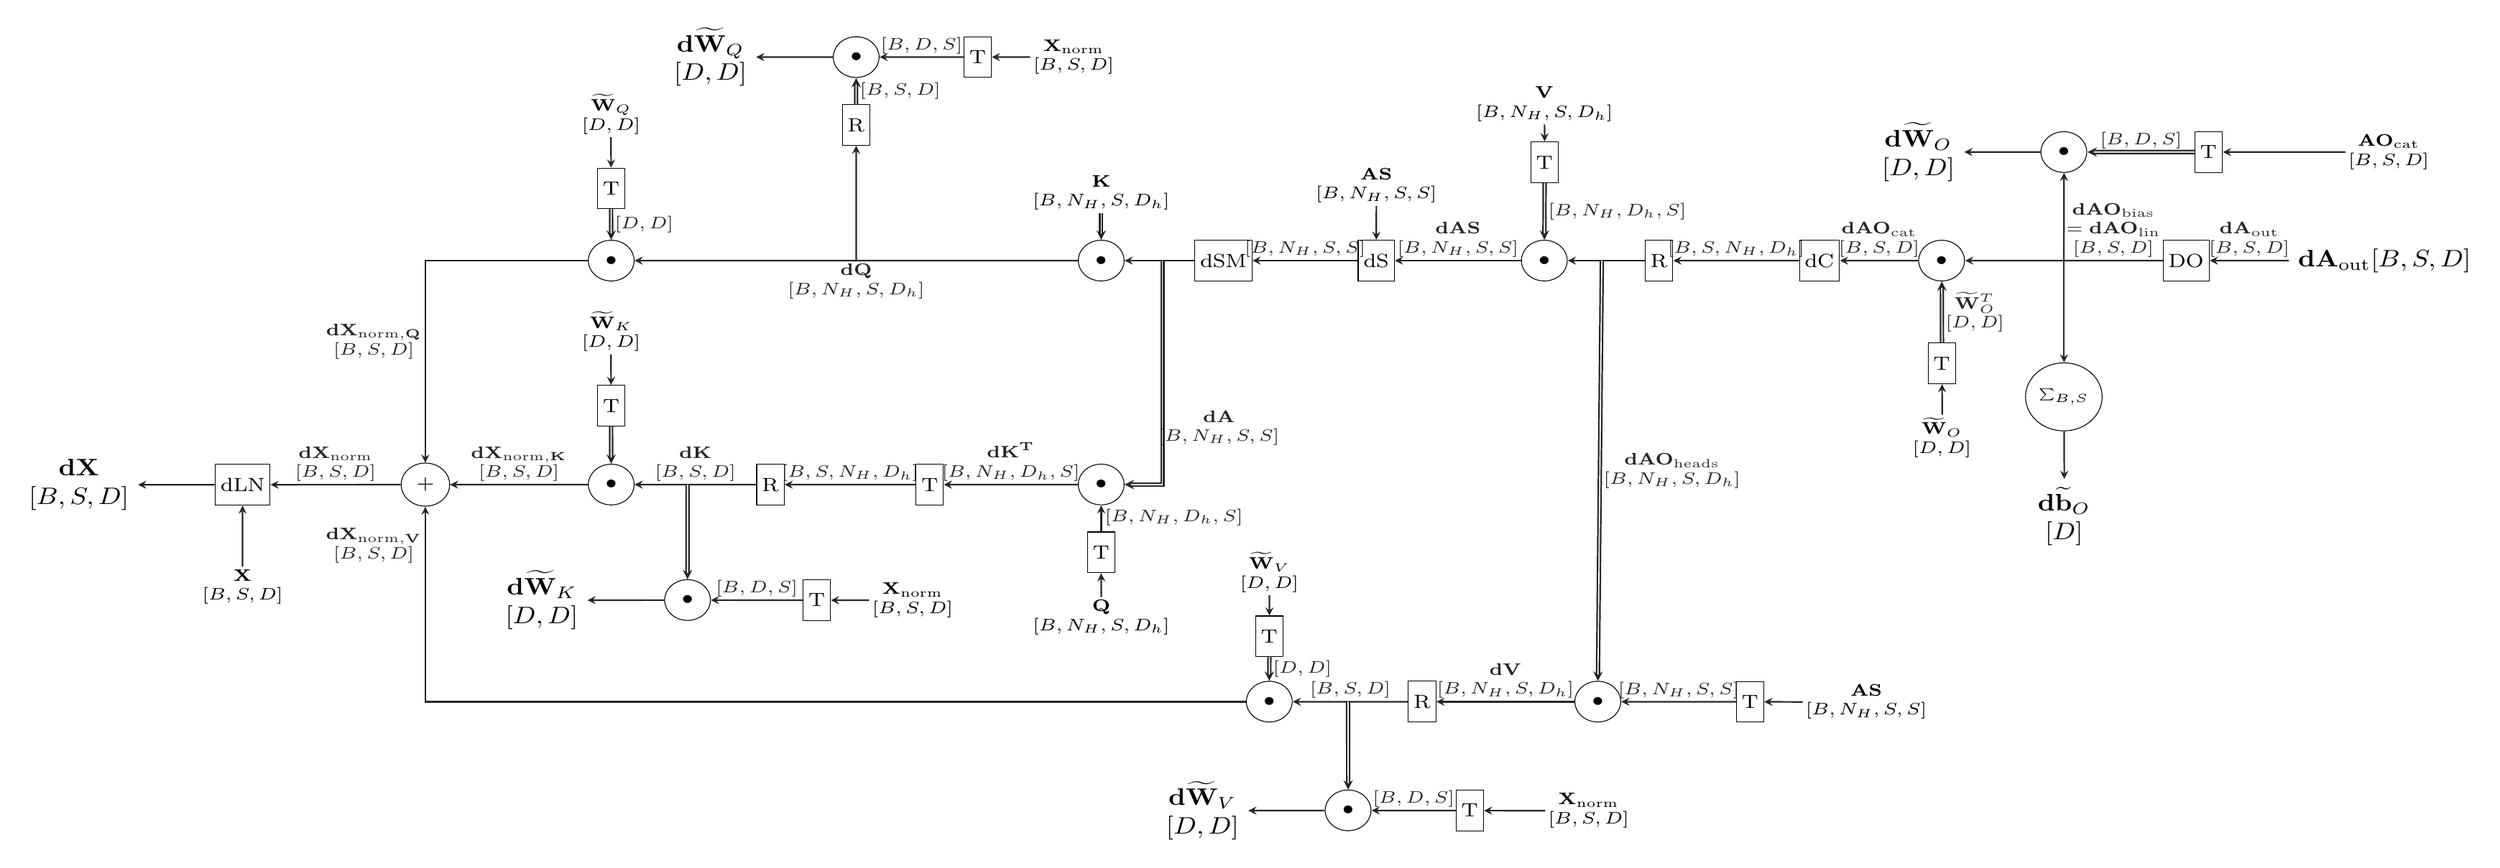
\begin{tikzpicture}[
  every node/.style={transform shape},
  >=stealth,
  auxnode/.style={draw, rectangle, fill=white, minimum height=6mm, inner sep=2pt, font=\footnotesize, align=center},
  mulnode/.style={draw, circle, fill=white, minimum size=6mm, font=\footnotesize, align=center},
  addnode/.style={draw, circle, fill=white, minimum size=6mm, font=\footnotesize, align=center},
  sumnode/.style={draw, circle, fill=white, minimum size=6mm, font=\tiny, align=center},
  flow/.style={->, thick, black!85},
  flow2/.style={->, double, thick, black!85},
  dimlabel/.style={font=\scriptsize, inner sep=1pt, align=center},
  gradflow/.style={->, thick, black!85},
  gradweight/.style={->, thick, black!85}
]

\begin{scope}[xscale=1.35, yscale=1.2]

\def\yoffset{-1.0}
\def\dVXyoffset{-6.5}

\coordinate (Grad_Aout_B) at (17.5, \yoffset);
\coordinate (dDrop_center) at (15.9, \yoffset);
\coordinate (ProjGradSplit) at (14.3, \yoffset);
\coordinate (dOProj_center) at (12.7, \yoffset);
\coordinate (C_center) at (11.1, \yoffset);
\coordinate (R_center) at (9.0, \yoffset);
\coordinate (dPV_AS_calc_center) at (7.5, \yoffset);
\coordinate (dSoft_center) at (5.3, \yoffset);
\coordinate (dSM_calc_center) at (3.3, \yoffset);
\coordinate (dV_calc_center) at (8.2, \dVXyoffset+\yoffset);
\coordinate (R_V_bwd_center) at (5.9, \dVXyoffset+\yoffset);
\coordinate (dVX_calc_center) at (3.9, \dVXyoffset+\yoffset);
\coordinate (dQK_calc_Q_center) at (1.7, \yoffset);
\coordinate (dQK_calc_K_center) at (1.7, -3.3+\yoffset);
\coordinate (K_BWD_input_center) at (1.7, 1.0+\yoffset);
\coordinate (T_Q_bwd_center) at (1.7, -4.3+\yoffset);

% \node[font=\Large\bfseries] at (8, 4.6+\yoffset) {Multi-Head Attention Backward Pass};

\node (Grad_Aout_B) at (18.5, \yoffset) {$\mathbf{dA}_{\text{out}}$\\$[B,S,D]$};
\node[auxnode] (DO) at (dDrop_center) {DO};
\node[mulnode] (dOProj) at (dOProj_center) {$\bullet$};

\node[auxnode] (T_WO) [below=0.9cm of dOProj] {T};
\node[dimlabel] (WO_BWD) [below=0.45cm of T_WO] {$\widetilde{\mathbf{W}}_{O}$\\$[D,D]$};

\node[mulnode] (dWO_calc) at ($(ProjGradSplit)+(0, 1.6)$) {$\bullet$};
\node[align=center, left=1.0cm of dWO_calc]
  (dWO_GRAD) {$\mathbf{d}\widetilde{\mathbf{W}}_{O}$\\$[D,D]$};
\node[auxnode] (T_AO_in) [right=1.4cm of dWO_calc] {T};
\node[dimlabel] (AO_in_local_label) [right=1.6cm of T_AO_in] {$\mathbf{AO}_{\text{cat}}$\\$[B,S,D]$};

\node[auxnode] (C) at (C_center) {dC};
\node[auxnode] (R) at (R_center) {R};

\node[mulnode] (dPV_AS_calc) at (dPV_AS_calc_center) {$\bullet$};
\node[auxnode] (dSoft) at (dSoft_center) {dS};
\node[auxnode] (dSM_calc) at (dSM_calc_center) {dSM};

\node[mulnode] (dQK_calc_Q) at (dQK_calc_Q_center) {$\bullet$};
\node[mulnode] (dQX_proj_calc) [left=5.8cm of dQK_calc_Q] {$\bullet$};

\node[mulnode] (dQK_calc_K) at (dQK_calc_K_center) {$\bullet$};
\node[mulnode] (dKX_proj_calc) [left=5.8cm of dQK_calc_K] {$\bullet$};

\node[dimlabel] (K_BWD_input) at (K_BWD_input_center) {$\mathbf{K}$\\$[B,N_H,S,D_h]$};
\node[auxnode] (T_Q_bwd) at (T_Q_bwd_center) {T};
\node[dimlabel] (Q_BWD_input) [below=0.35cm of T_Q_bwd] {$\mathbf{Q}$\\$[B,N_H,S,D_h]$};

\node[dimlabel] (V_FWD) [above=1.7cm of dPV_AS_calc] {$\mathbf{V}$\\$[B,N_H,S,D_h]$};
\node[auxnode] (T_V_bwd) [below=0.25cm of V_FWD] {T};

\node[mulnode] (dV_calc) at (dV_calc_center) {$\bullet$};
\node[auxnode] (T_AS_bwd) [right=1.5cm of dV_calc] {T};
\node[dimlabel] (AS_BWD_for_V) [right=0.5cm of T_AS_bwd] {$\mathbf{AS}$\\$[B,N_H,S,S]$};

\node[auxnode] (R_V_bwd) at (R_V_bwd_center) {R};
\node[mulnode] (dVX_calc) at (dVX_calc_center) {$\bullet$};

\node[auxnode] (T_WV) [above=0.35cm of dVX_calc] {T};
\node[dimlabel] (WV_BWD) [above=0.3cm of T_WV] {$\widetilde{\mathbf{W}}_{V}$\\$[D,D]$};

\node[sumnode] (Sum_dBO) [below=1.5cm of ProjGradSplit] {$\sum_{B, S}$};
\node (dBO) [align=center, below=0.7cm of Sum_dBO] {$\mathbf{d}\widetilde{\mathbf{b}}_{O}$\\$[D]$};

\draw[gradflow] (Grad_Aout_B) -- (DO)
  node[dimlabel, midway, above]{$\mathbf{dA}_{\text{out}}$\\$[B,S,D]$};

\draw[gradflow] (DO) -- (dOProj)
  node[dimlabel, pos=0.25, above]{$\mathbf{dAO}_{\text{bias}}$\\$=\mathbf{dAO}_{\text{lin}}$\\$[B,S,D]$};

\draw[gradflow] (ProjGradSplit) -- (dWO_calc.south);
\draw[gradflow] (ProjGradSplit) -- ([yshift=-0.75cm]ProjGradSplit) -| (Sum_dBO.north);

\draw[gradflow] (dOProj) -- (C)
  node[dimlabel, midway, above]{$\mathbf{dAO}_{\text{cat}}$\\$[B,S,D]$};
\draw[gradflow] (C) -- (R)
  node[dimlabel, midway, above]{$[B,S,N_H,D_h]$};

\coordinate (R_split_point) at ($(dPV_AS_calc)!0.5!(R)$);
\draw[gradflow] (R.west) -- (dPV_AS_calc.east);
\draw[flow2] (R_split_point) -- (dV_calc.north)
  node[dimlabel, midway, right]{$\mathbf{dAO}_{\text{heads}}$\\$[B,N_H,S,D_h]$};

\draw[gradflow] (V_FWD.south) -- (T_V_bwd.north);
\draw[flow2] (T_V_bwd.south) -- (dPV_AS_calc.north)
  node[dimlabel, midway, right]{$[B,N_H,D_h,S]$};
\draw[gradflow] (dPV_AS_calc.west) -- (dSoft.east)
  node[dimlabel, midway, above]{$\mathbf{dAS}$\\$[B,N_H,S,S]$};

\node (AS_BWD_dS) [dimlabel, above=0.5cm of dSoft] {$\mathbf{AS}$\\$[B,N_H,S,S]$};
\draw[gradflow] (AS_BWD_dS.south) -- (dSoft.north);
\draw[gradflow] (dSoft.west) -- (dSM_calc.east)
  node[dimlabel, midway, above]{$[B,N_H,S,S]$};

\coordinate (dA_Split_X) at ($(dSM_calc_center)!0.5!(dQK_calc_Q_center)$);
\coordinate (dA_Split) at (dA_Split_X |- dQK_calc_Q.east);
\draw[gradflow] (dSM_calc.west) -- (dQK_calc_Q.east);
\draw[flow2] (dA_Split) -- (dA_Split |- dQK_calc_K.east) -- (dQK_calc_K.east)
  node[dimlabel, pos=-1.5, above, yshift=15]{$\mathbf{dA}$\\$[B,N_H,S,S]$};

\draw[flow2] (K_BWD_input.south) -- (dQK_calc_Q.north);
\draw[gradweight] (dQK_calc_Q) -- (dQX_proj_calc)
  node[dimlabel, midway, below]{$\mathbf{dQ}$\\$[B,N_H,S,D_h]$};

\node[auxnode] (T_WQ_bwd) [above=0.45cm of dQX_proj_calc] {T};
\node[dimlabel] (WQ_bwd) [above=0.45cm of T_WQ_bwd] {$\widetilde{\mathbf{W}}_{Q}$\\$[D,D]$};
\draw[flow] (WQ_bwd) -- (T_WQ_bwd);
\draw[flow2] (T_WQ_bwd.south) -- (dQX_proj_calc.north)
  node[dimlabel, midway, right]{$[D,D]$};

\draw[flow] (Q_BWD_input.north) -- (T_Q_bwd.south);
\draw[flow] (T_Q_bwd.north) -- (dQK_calc_K.south)
  node[dimlabel, pos=0.55, right]{$[B,N_H,D_h,S]$};

\node[auxnode] (T_dK) at ($(dQK_calc_K)!0.35!(dKX_proj_calc)$) {T};
\node[auxnode] (R_dK_mid) at ($(T_dK)!0.5!(dKX_proj_calc)$) {R};

\draw[gradweight] (dQK_calc_K) -- (T_dK)
  node[dimlabel, midway, above]{$\mathbf{dK^T}$\\$[B,N_H,D_h,S]$};
\draw[gradweight] (T_dK) -- (R_dK_mid)
  node[dimlabel, midway, above]{$[B,S,N_H,D_h]$};
\draw[gradweight] (R_dK_mid) -- (dKX_proj_calc)
  node[dimlabel, midway, above]{$\mathbf{dK}$\\$[B,S,D]$};

\node[auxnode] (T_WK_bwd) [above=0.55cm of dKX_proj_calc] {T};
\node[dimlabel] (WK_bwd) [above=0.45cm of T_WK_bwd] {$\widetilde{\mathbf{W}}_{K}$\\$[D,D]$};
\draw[gradflow] (WK_bwd) -- (T_WK_bwd);
\draw[flow2] (T_WK_bwd.south) -- (dKX_proj_calc.north);

\draw[gradflow] (AS_BWD_for_V.west) -- (T_AS_bwd.east);
\draw[gradflow] (T_AS_bwd.west) -- (dV_calc.east)
  node[dimlabel, midway, above]{$[B,N_H,S,S]$};
\draw[gradflow] (dV_calc.west) -- (R_V_bwd.east)
  node[dimlabel, midway, above]{$\mathbf{dV}$\\$[B,N_H,S,D_h]$};
\draw[gradflow] (R_V_bwd) -- (dVX_calc.east)
  node[dimlabel, midway, above]{$[B,S,D]$};

\draw[gradflow] (WV_BWD) -- (T_WV);
\draw[flow2] (T_WV) -- (dVX_calc.north)
  node[dimlabel, midway, right]{$[D,D]$};

\node[addnode] (Sum_dXnorm) [left=1.8cm of dKX_proj_calc] {$+$};

\draw[gradweight] (dQX_proj_calc.west) -| node[dimlabel, pos=0.7, left]{$\mathbf{dX}_{\text{norm},\mathbf{Q}}$\\$[B,S,D]$} (Sum_dXnorm.north);
\draw[gradweight] (dKX_proj_calc.west) -- node[dimlabel, midway, above]{$\mathbf{dX}_{\text{norm},\mathbf{K}}$\\$[B,S,D]$} (Sum_dXnorm.east);
\draw[gradweight] (dVX_calc.west) -| node[dimlabel, pos=0.9, left]{$\mathbf{dX}_{\text{norm},\mathbf{V}}$\\$[B,S,D]$} (Sum_dXnorm.south);

\coordinate (dV_branch) at ($(R_V_bwd.west)!0.52!(dVX_calc.east)$);
\node[mulnode] (dWV_mul) at ($(dV_branch)+(0,-1.6cm)$) {$\bullet$};
\draw[flow2] (dV_branch) -- (dWV_mul.north);

\node[auxnode] (T_Xnorm) [right=1.1cm of dWV_mul] {T};
\node[dimlabel] (Xnorm_local) [right=0.8cm of T_Xnorm] {$\mathbf{X}_{\text{norm}}$\\$[B,S,D]$};
\draw[gradflow] (Xnorm_local) -- (T_Xnorm);
\draw[gradflow] (T_Xnorm.west) -- (dWV_mul.east)
  node[dimlabel, midway, above]{$[B,D,S]$};
\node (dWV_out) [align=center, left=1.0cm of dWV_mul] {$\mathbf{d}\widetilde{\mathbf{W}}_{V}$\\$[D,D]$};
\draw[gradweight] (dWV_mul.west) -- (dWV_out);

\coordinate (dQ_branch) at ($(dQK_calc_Q.east)!0.50!(dQX_proj_calc.west)$);
\node[mulnode] (dWQ_mul) at ($(dQ_branch)+(0,3.0cm)$) {$\bullet$};
\node[auxnode] (R_dQ_for_WQ) at ($(dWQ_mul)+(0,-1.0cm)$) {R};
\draw[gradflow]  (dQ_branch) -- (R_dQ_for_WQ.south);
\draw[flow2] (R_dQ_for_WQ.north) -- (dWQ_mul.south)
  node[dimlabel, midway, right]{$[B,S,D]$};

\node[auxnode] (T_XnormQ) [right=1.1cm of dWQ_mul] {T};
\node[dimlabel] (Xnorm_localQ) [right=0.5cm of T_XnormQ] {$\mathbf{X}_{\text{norm}}$\\$[B,S,D]$};
\draw[gradflow] (Xnorm_localQ) -- (T_XnormQ);
\draw[gradflow] (T_XnormQ.west) -- (dWQ_mul.east)
  node[dimlabel, midway, above]{$[B,D,S]$};
\node (dWQ_out) [align=center, left=1.0cm of dWQ_mul] {$\mathbf{d}\widetilde{\mathbf{W}}_{Q}$\\$[D,D]$};
\draw[gradweight] (dWQ_mul.west) -- (dWQ_out);

\coordinate (dK_branch) at ($(R_dK_mid)!0.52!(dKX_proj_calc)$);
\node[mulnode] (dWK_mul) at ($(dK_branch)+(0,-1.7cm)$) {$\bullet$};
\draw[flow2]  (dK_branch) -- (dWK_mul.north);

\node[auxnode] (T_XnormK) [right=1.2cm of dWK_mul] {T};
\node[dimlabel, right=0.5cm of T_XnormK] (Xnorm_localK) {$\mathbf{X}_{\text{norm}}$\\$[B,S,D]$};
\draw[gradflow] (Xnorm_localK) -- (T_XnormK);
\draw[gradflow] (T_XnormK.west) -- (dWK_mul.east)
  node[dimlabel, midway, above]{$[B,D,S]$};
\node (dWK_out) [align=center, left=1.0cm of dWK_mul] {$\mathbf{d}\widetilde{\mathbf{W}}_{K}$\\$[D,D]$};
\draw[gradweight] (dWK_mul.west) -- (dWK_out);

\draw[gradweight] (Sum_dBO) -- (dBO);

\draw[gradflow] (WO_BWD) -- (T_WO);
\draw[flow2] (T_WO) -- (dOProj)
  node[dimlabel, midway, right]{$\widetilde{\mathbf{W}}_{O}^{T}$\\$[D,D]$};
\draw[gradflow] (AO_in_local_label) -- (T_AO_in);
\draw[flow2] (T_AO_in) -- (dWO_calc.east)
  node[dimlabel, midway, above]{$[B,D,S]$};
\draw[gradweight] (dWO_calc) -- (dWO_GRAD);

\node[auxnode] (dLN) [left=1.7cm of Sum_dXnorm] {dLN};
\draw[gradweight] (Sum_dXnorm.west) -- node[dimlabel, midway, above]
  {$\mathbf{dX}_{\text{norm}}$\\$[B,S,D]$} (dLN.east);

\node (dX_OUT) [align=center, left=1.0cm of dLN] {$\mathbf{dX}$\\$[B,S,D]$};
\draw[gradweight] (dLN.west) -- (dX_OUT);

\node[dimlabel] (LNCache) [below=0.9cm of dLN] {$\mathbf{X}$\\$[B,S,D]$};
\draw[gradflow] (LNCache.north) -- (dLN.south);

\end{scope}
\end{tikzpicture}
}

\end{landscape}
\clearpage

% ------------------------ 4.3 MLP / FFN Block ------------------------
\subsection{Feed-Forward Network (MLP / FFN)}

\subsubsection{Forward Pass}
\resizebox{\linewidth}{!}{%
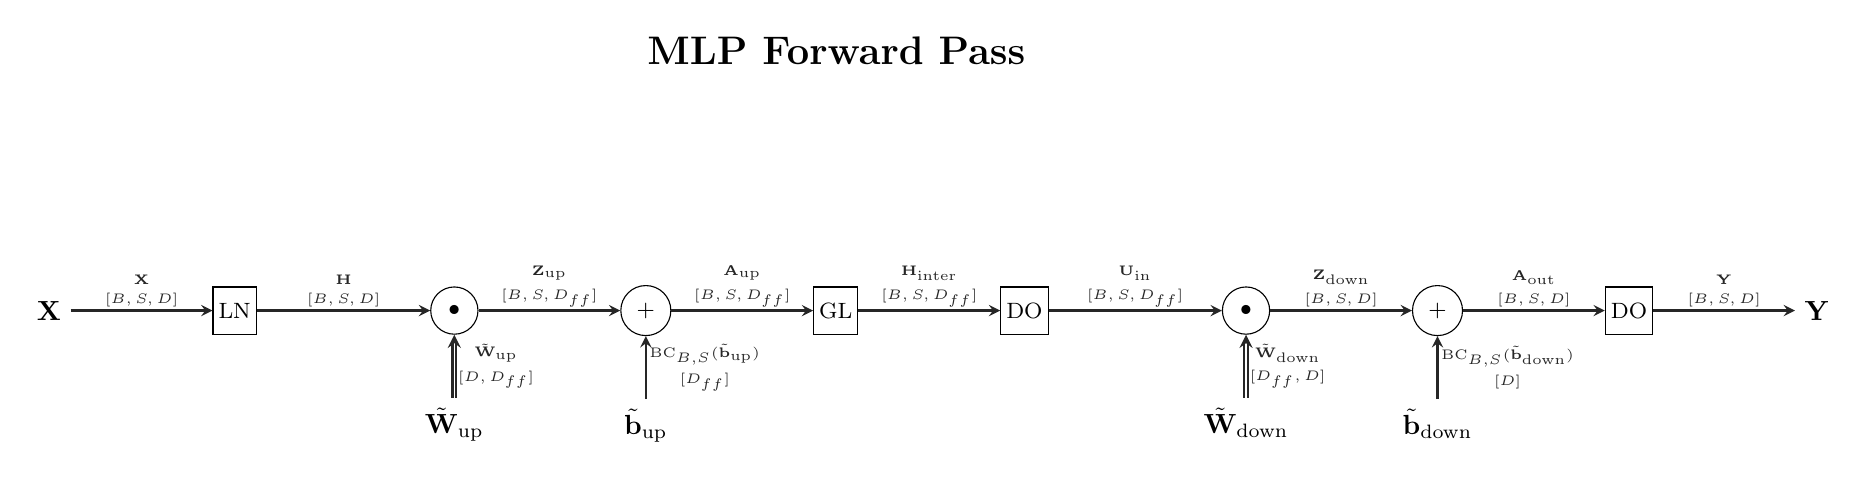
\begin{tikzpicture}[
    >=stealth,
    auxnode/.style={draw, rectangle, fill=white, minimum height=6mm, inner sep=2pt, font=\footnotesize, align=center},
    mulnode/.style={draw, circle, fill=white, minimum size=6mm, font=\footnotesize, align=center},
    addnode/.style={draw, circle, fill=white, minimum size=6mm, font=\footnotesize, align=center},
    sumnode/.style={draw, circle, fill=white, minimum size=6mm, font=\tiny, align=center},
    flow/.style={->, thick, black!85},
    flow2/.style={double, ->, thick, black!85},
    dimlabel/.style={font=\tiny, inner sep=1pt, align=center}
]
    \node[font=\Large\bfseries] at (10, 2.8) {MLP Forward Pass};

    \pgfmathsetmacro{\verticaloffset}{-0.5}

    \node            (MIn)   at (0,\verticaloffset) {$\mathbf{X}$};
    \node[auxnode]   (LN2)   [right=1.8cm of MIn] {LN};
    \node[mulnode]   (L1Mul) [right=2.2cm of LN2] {$\bullet$};
    \node            (Wup)   [below=0.8cm of L1Mul] {$\tilde{\mathbf{W}}_{\text{up}}$};
    \node[addnode]   (AddB1) [right=1.8cm of L1Mul] {+};
    \node            (Bup)   [below=0.8cm of AddB1] {$\tilde{\mathbf{b}}_{\text{up}}$};
    \node[auxnode]   (Act)   [right=1.8cm of AddB1] {GL};
    \node[auxnode]   (Drop1) [right=1.8cm of Act] {DO};
    \node[mulnode]   (L2Mul) [right=2.2cm of Drop1] {$\bullet$};
    \node            (Wdown) [below=0.8cm of L2Mul] {$\tilde{\mathbf{W}}_{\text{down}}$};
    \node[addnode]   (AddB2) [right=1.8cm of L2Mul] {+};
    \node            (Bdown) [below=0.8cm of AddB2] {$\tilde{\mathbf{b}}_{\text{down}}$};
    \node[auxnode]   (Drop2) [right=1.8cm of AddB2] {DO};
    \node            (MOut)  [right=1.8cm of Drop2] {$\mathbf{Y}$};

    \draw[flow] (MIn) -- (LN2) node[dimlabel, midway, above]{\shortstack{$\mathbf{X}$\\$[B,S,D]$}};
    \draw[flow] (LN2) -- (L1Mul) node[dimlabel, midway, above]{\shortstack{$\mathbf{H}$\\$[B,S,D]$}};
    \draw[flow2] (Wup) -- (L1Mul) node[dimlabel, midway, right]{\shortstack{$\tilde{\mathbf{W}}_{\text{up}}$\\$[D, D_{ff}]$}};
    \draw[flow] (L1Mul) -- (AddB1) node[dimlabel, midway, above]{\shortstack{$\mathbf{Z}_{\text{up}}$\\$[B,S,D_{ff}]$}};
    \draw[flow] (Bup) -- (AddB1) node[dimlabel, midway, right]{\shortstack{$\mathrm{BC}_{B,S}(\tilde{\mathbf{b}}_{\text{up}})$\\$[D_{ff}]$}};
    \draw[flow] (AddB1) -- (Act) node[dimlabel, midway, above]{\shortstack{$\mathbf{A}_{\text{up}}$\\$[B,S,D_{ff}]$}};
    \draw[flow] (Act) -- (Drop1) node[dimlabel, midway, above]{\shortstack{$\mathbf{H}_{\text{inter}}$\\$[B,S,D_{ff}]$}};
    \draw[flow] (Drop1) -- (L2Mul) node[dimlabel, midway, above]{\shortstack{$\mathbf{U}_{\text{in}}$\\$[B,S,D_{ff}]$}};
    \draw[flow2] (Wdown) -- (L2Mul) node[dimlabel, midway, right]{\shortstack{$\tilde{\mathbf{W}}_{\text{down}}$\\$[D_{ff}, D]$}};
    \draw[flow] (L2Mul) -- (AddB2) node[dimlabel, midway, above]{\shortstack{$\mathbf{Z}_{\text{down}}$\\$[B,S,D]$}};
    \draw[flow] (Bdown) -- (AddB2) node[dimlabel, midway, right]{\shortstack{$\mathrm{BC}_{B,S}(\tilde{\mathbf{b}}_{\text{down}})$\\$[D]$}};
    \draw[flow] (AddB2) -- (Drop2) node[dimlabel, midway, above]{\shortstack{$\mathbf{A}_{\text{out}}$\\$[B,S,D]$}};
    \draw[flow] (Drop2) -- (MOut) node[dimlabel, midway, above]{\shortstack{$\mathbf{Y}$\\$[B,S,D]$}};

\end{tikzpicture}%
}


\clearpage

\subsubsection{Backward Pass}
\noindent
\resizebox{\linewidth}{!}{%
\begin{tikzpicture}[
    >=stealth,
    auxnode/.style={draw, rectangle, fill=white, minimum height=6mm, inner sep=2pt, font=\footnotesize, align=center},
    mulnode/.style={draw, circle, fill=white, minimum size=6mm, font=\footnotesize, align=center},
    addnode/.style={draw, circle, fill=white, minimum size=6mm, font=\footnotesize, align=center},
    sumnode/.style={draw, circle, fill=white, minimum size=6mm, font=\tiny, align=center},
    flow_rev/.style={<-, thick, black!85},
    flow_dw/.style={->, thick, black!85},
    flow_act/.style={double, ->, thick, black!85},
    dimlabel/.style={font=\tiny, inner sep=1pt, align=center},
    gradlabel/.style={font=\tiny\bfseries, inner sep=1pt, align=center}
]
    \node[font=\Large\bfseries] at (5, 10) {MLP Backward Pass};

    \pgfmathsetmacro{\backwardoffset}{0.0}

    \node (d_MOut) at (12.6, \backwardoffset) {$\mathrm{d}\mathbf{Y}$};
    \node[auxnode] (d_Drop2) [left=1.8cm of d_MOut] {dDO};
    \draw[flow_rev] (d_Drop2) -- (d_MOut)
      node[dimlabel, midway, below]{\shortstack{$\mathrm{d}\mathbf{Y}$\\$[B,S,D]$}};

    \coordinate (split2) at ($(d_Drop2.west) + (-1.5cm, 0)$);
    \coordinate (branch_dUproj) at ($(split2) + (-1.2cm, 0)$);

    \node[sumnode] (d_SumB2) [above=0.8cm of split2] {$\sum_{B, S}$};
    \node (d_Bdown) [above=0.8cm of d_SumB2] {$\mathrm{d}\tilde{\mathbf{b}}_{\text{down}}$};
    \draw[flow_dw] (d_SumB2) -- (d_Bdown) node[dimlabel, midway, right]{$[D]$};

    \draw[flow_rev] (split2) -- (d_Drop2);
    \draw[flow_rev] (d_SumB2) -- (split2);

    \node[mulnode] (d_L2Mul_in) [left=2.2cm of split2] {$\bullet$};
    \draw[flow_rev] (d_L2Mul_in) -- (d_Drop2)
      node[gradlabel, midway, below]{\shortstack{$\mathrm{d}\mathbf{Z}_{\text{down}}=\mathrm{d}\mathbf{A}_{\text{out}}$\\$[B,S,D]$}};

    \node (W_down_T) [below=1.8cm of d_L2Mul_in] {$\tilde{\mathbf{W}}_{\text{down}}^{T}$};
    \draw[flow_act] (W_down_T.north) -- (d_L2Mul_in)
      node[dimlabel, midway, right]{$[D, D_{ff}]$};

    \coordinate (L2Mul_w_y) at ($(d_L2Mul_in) + (0, 3.5cm)$);
    \node[mulnode] (d_L2Mul_w) at (L2Mul_w_y) {$\bullet$};
    \node (d_Wdown) [above=0.8cm of d_L2Mul_w] {$\mathrm{d}\tilde{\mathbf{W}}_{\text{down}}$};
    \draw[flow_dw] (d_L2Mul_w) -- (d_Wdown) node[dimlabel, midway, right]{$[D_{ff}, D]$};

    \draw[flow_act] (branch_dUproj.north) |- (d_L2Mul_w.east);

    \node[auxnode] (Uin_T) at ($(d_L2Mul_w.west) + (-1.5cm, 0)$) {T};
    \draw[flow_dw] (Uin_T) -- (d_L2Mul_w)
      node[dimlabel, midway, below]{\shortstack{$\mathbf{U}_{\text{in}}^T$\\$[B, D_{ff}, S]$}};
    \node (Uin_aux) [left=1.8cm of Uin_T] {$\mathbf{U}_{\text{in}}$};
    \draw[flow_dw] (Uin_aux) -- (Uin_T) node[dimlabel, midway, above]{\shortstack{$[B,S,D_{ff}]$}};

    \node[auxnode] (d_Drop1) [left=1.8cm of d_L2Mul_in] {dDO};
    \draw[flow_rev] (d_Drop1) -- (d_L2Mul_in)
      node[dimlabel, midway, below]{\shortstack{$\mathrm{d}\mathbf{U}_{\text{in}}$\\$[B,S,D_{ff}]$}};

    \node[auxnode] (d_Act) [left=1.8cm of d_Drop1] {dGL};
    \draw[flow_rev] (d_Act) -- (d_Drop1)
      node[dimlabel, midway, below]{\shortstack{$\mathrm{d}\mathbf{H}_{\text{inter}}$\\$[B,S,D_{ff}]$}};

    \coordinate (split1) at ($(d_Act.west) + (-1.5cm, 0)$);
    \coordinate (branch_dHpre) at ($(split1) + (-1.2cm, 0)$);

    \node[sumnode] (d_SumB1) [above=0.8cm of split1] {$\sum_{B, S}$};
    \node (d_Bup) [above=0.8cm of d_SumB1] {$\mathrm{d}\tilde{\mathbf{b}}_{\text{up}}$};
    \draw[flow_dw] (d_SumB1) -- (d_Bup) node[dimlabel, midway, right]{$[D_{ff}]$};

    \draw[flow_rev] (split1) -- (d_Act);
    \draw[flow_rev] (d_SumB1) -- (split1);

    \node[mulnode] (d_L1Mul_in) [left=2.2cm of split1] {$\bullet$};
    \draw[flow_rev] (d_L1Mul_in) -- (d_Act)
      node[gradlabel, midway, below]{\shortstack{$\mathrm{d}\mathbf{Z}_{\text{up}}=\mathrm{d}\mathbf{A}_{\text{up}}$\\$[B,S,D_{ff}]$}};

    \node (W_up_T) [below=1.8cm of d_L1Mul_in] {$\tilde{\mathbf{W}}_{\text{up}}^{T}$};
    \draw[flow_act] (W_up_T.north) -- (d_L1Mul_in)
      node[dimlabel, midway, right]{$[D_{ff}, D]$};

    \coordinate (L1Mul_w_y) at ($(d_L1Mul_in) + (0, 3.5cm)$);
    \node[mulnode] (d_L1Mul_w) at (L1Mul_w_y) {$\bullet$};
    \node (d_Wup) [above=0.8cm of d_L1Mul_w] {$\mathrm{d}\tilde{\mathbf{W}}_{\text{up}}$};
    \draw[flow_dw] (d_L1Mul_w) -- (d_Wup) node[dimlabel, midway, right]{$[D, D_{ff}]$};

    \draw[flow_act] (branch_dHpre.north) |- (d_L1Mul_w.east);

    \node[auxnode] (Znorm_T) at ($(d_L1Mul_w.west) + (-1.5cm, 0)$) {T};
    \draw[flow_dw] (Znorm_T) -- (d_L1Mul_w)
      node[dimlabel, midway, below]{\shortstack{$\mathbf{H}^T$\\$[B, D, S]$}};
    \node (Znorm_aux) [left=1.8cm of Znorm_T] {$\mathbf{H}$};
    \draw[flow_dw] (Znorm_aux) -- (Znorm_T) node[dimlabel, midway, above]{\shortstack{$[B,S,D]$}};

    \node[auxnode] (d_LN2) [left=1.8cm of d_L1Mul_in] {dLN};
    \draw[flow_rev] (d_LN2) -- (d_L1Mul_in)
      node[dimlabel, midway, below]{\shortstack{$\mathrm{d}\mathbf{H}$\\$[B,S,D]$}};

    \node (d_MIn) [left=1.8cm of d_LN2] {$\mathrm{d}\mathbf{X}$};
    \draw[flow_rev] (d_MIn) -- (d_LN2)
      node[dimlabel, midway, below]{\shortstack{$\mathrm{d}\mathbf{X}$\\$[B,S,D]$}};
\end{tikzpicture}%
}


\clearpage

% ------------------------ 4.4 Output Projection & Loss ---------------
\subsection{Output Projection and Loss}

\subsubsection{Forward Pass (Logits, Softmax, Loss)}

\noindent
\resizebox{\linewidth}{!}{%
\begin{tikzpicture}[
  >=stealth,
  auxnode/.style={draw, rectangle, fill=white, minimum height=6mm, inner sep=2pt, font=\footnotesize, align=center},
  mulnode/.style={draw, circle, fill=white, minimum size=6mm, font=\footnotesize, align=center},
  addnode/.style={draw, circle, fill=white, minimum size=6mm, font=\footnotesize, align=center},
  sumnode/.style={draw, circle, fill=white, minimum size=6mm, font=\tiny, align=center},
  flow/.style={->, thick, black!85},
  flow2/.style={double, ->, thick, black!85},
  dimlabel/.style={font=\tiny, inner sep=1pt, align=center}
]

% From Transformer output
\node            (H)     at (0,-2) {$\mathbf{A}_{\text{out}}$};

% LM head
\node[mulnode]   (LMmul) [right=2.2cm of H] {$\bullet$};
\node            (Wlm)   [align=center, below=0.9cm of LMmul] {$\widetilde{\mathbf{W}}_{\text{lm}}$\\$=\mathbf{E}^{T}$};
\node[addnode]   (AddB)  [right=1.8cm of LMmul] {+};
\node            (blm)   [below=0.9cm of AddB] {$\widetilde{\mathbf{b}}_{\text{lm}}$};

% Softmax → Prob
\node[auxnode]   (SM)    [right=1.8cm of AddB] {S};

\node[auxnode] (ARG)  [right=4.0cm of SM] {ARG};
% Midpoint of SM→P edge (for CE tap)
\coordinate (MidSP) at ($(SM)!0.5!(ARG)$);

% CE node placed below the SM→P edge
\node[auxnode]   (CE)    [below=1.6cm of MidSP] {CE};
\node            (Y)     [right=0.9cm of CE] {$\mathbf{Y_\text{targets}}$};
\node            (Loss)  [align=center, below=1.8cm of CE] {$\mathcal{L}$\\ (mean over $B,S$)};

% Flows
\draw[flow]  (H) -- (LMmul) node[dimlabel, midway, above]{\shortstack{$[B,S,D]$}};
\draw[flow2] (Wlm) -- (LMmul) node[dimlabel, midway, right]{\shortstack{$[D,V]$}};
\draw[flow]  (LMmul) -- (AddB) node[dimlabel, midway, above]{\shortstack{$\mathbf{Z}_{\text{lin}}$\\$[B,S,V]$}};
\draw[flow]  (blm) -- (AddB)   node[dimlabel, midway, right]{\shortstack{$\text{BC}_{B,S}(\widetilde{\mathbf{b}}_{\text{lm}})$\\$[V]$}};
\draw[flow]  (AddB) -- (SM)    node[dimlabel, midway, above]{\shortstack{\textbf{Z\textsubscript{bias}}\\ $[B,S,V]$}};

% Tap the SM→P edge downward into CE
\draw[flow]  (MidSP) -- (CE);
% Targets into CE
\draw[flow]  (Y) -- (CE)  node[dimlabel, midway, above]{\shortstack{targets\\$[B,S]$}};
% Loss goes WEST (left) from CE
\draw[flow]  (CE) -- (Loss);

\node (YhatG) [right=1.8cm of ARG] {$\hat{\mathbf{Y}}_{\text{greedy}}$};
\draw[flow] (SM) -- (ARG)
  node[dimlabel, pos=0.35, above]{\shortstack{$\mathbf{P}$\\$[B,S,V]$}};
\draw[flow] (ARG) -- (YhatG)
  node[dimlabel, midway, above]{\shortstack{token ids\\$[B,S]$}};

% Optional: top-k (or nucleus) sampling path
\node[auxnode] (TopK) [above=1.4cm of ARG] {TOP-$k$};
\node          (YhatS) [right=1.8cm of TopK] {$\hat{\mathbf{Y}}_{\text{sample}}$};
\draw[flow] (MidSP) |- (TopK);
\draw[flow] (TopK) -- (YhatS)
  node[dimlabel, midway, above]{\shortstack{token ids\\$[B,S]$}};

\node[font=\large\bfseries] at (9.2,1.8) {Token Generation \& Loss (Forward)};
\end{tikzpicture}%
}


\clearpage

\subsubsection{Backward Pass}
\noindent
\resizebox{0.8\linewidth}{!}{%
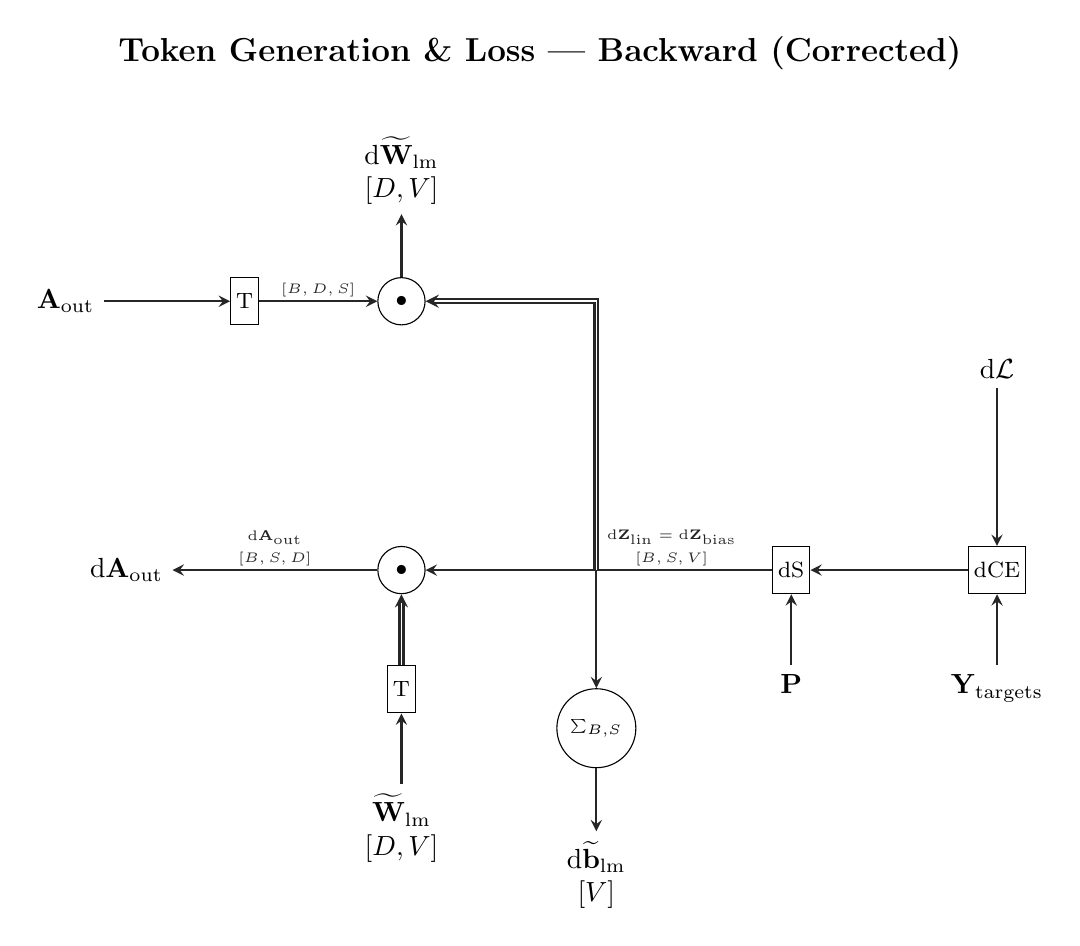
\begin{tikzpicture}[
  >=stealth,
  auxnode/.style={draw, rectangle, fill=white, minimum height=6mm, inner sep=2pt, font=\footnotesize, align=center},
  mulnode/.style={draw, circle, fill=white, minimum size=6mm, font=\footnotesize, align=center},
  addnode/.style={draw, circle, fill=white, minimum size=6mm, font=\footnotesize, align=center},
  sumnode/.style={draw, circle, fill=white, minimum size=6mm, font=\tiny, align=center},
  flow/.style={<-, thick, black!85},
  flow2/.style={double, <-, thick, black!85},
  fwd/.style={->, thick, black!85},
  gradflow/.style={->, thick, black!85},
  dimlabel/.style={font=\tiny, inner sep=1pt, align=center}
]

% Start from dL
\node           (dL)    at (18,0) {$\text{d}\mathcal{L}$};
\node[auxnode]  (dCE)   [below=2.0cm of dL] {dCE};
\node           (Y)     [below=0.9cm of dCE] {$\mathbf{Y_\text{targets}}$};

% Softmax backward
\node[auxnode]  (dS)   [left=2.0cm of dCE] {dS};
\node           (P)     [below=0.9cm of dS] {$\mathbf{P}$};

% Logits (Linear Projection) backprop node
\node[mulnode]  (backMul) [left=4.4cm of dS] {$\bullet$};
\node[auxnode]  (T_Wlm)   [below=0.9cm of backMul] {T};
\node           (Wlm)     [align=center, below=0.9cm of T_Wlm] {$\widetilde{\mathbf{W}}_{\text{lm}}$\\$[D,V]$};

\coordinate (B_split) at ($(backMul)!0.5!(dS)$);

% SUM node for Bias gradient
\node[sumnode]  (SumB) [below=1.5cm of B_split] {$\sum_{B,S}$};
\node           (db)   [align=center, below=0.8cm of SumB] {$\text{d}\widetilde{\mathbf{b}}_{\text{lm}}$\\$[V]$};

% dW calc
\node[mulnode]  (dWmul) [above=2.8cm of backMul] {$\bullet$};
\node[auxnode]  (TAout) [left=1.5cm of dWmul] {T};
\node           (Aout)  [left=1.6cm of TAout] {$\mathbf{A}_{\text{out}}$};
\node           (dW)    [align=center, above=0.8cm of dWmul] {$\text{d}\widetilde{\mathbf{W}}_{\text{lm}}$\\$[D,V]$};

% Back to Transformer
\node           (dH)    [left=2.6cm of backMul] {$\text{d}\mathbf{A}_{\text{out}}$};

% Flows
\draw[flow] (dCE) -- (dL);
\draw[fwd]  (Y) -- (dCE);
\draw[flow] (dS) -- (dCE);
\draw[fwd]  (P) -- (dS);

% Bias grad
\draw[gradflow] (B_split) -- (SumB.north);
\draw[gradflow] (SumB) -- (db);

% Linear projection backprop
\draw[flow] (backMul) -- (dS)
  node[dimlabel, pos=0.71, above]{\shortstack{$\text{d}\mathbf{Z}_{\text{lin}}=\text{d}\mathbf{Z}_{\text{bias}}$\\$[B,S,V]$}};
\draw[flow2] (backMul) -- (T_Wlm);
\draw[fwd]   (Wlm) -- (T_Wlm);
\draw[flow]  (dH) -- (backMul) node[dimlabel, midway, above]{\shortstack{$\text{d}\mathbf{A}_{\text{out}}$\\$[B,S,D]$}};

% dW calculation
\draw[gradflow] (dWmul) -- (dW);
\draw[fwd]  (Aout) -- (TAout);
\draw[fwd]  (TAout) -- (dWmul) node[dimlabel, midway, above]{\shortstack{$[B,D,S]$}};
\draw[flow2] (dWmul) -| (B_split);

\node[font=\large\bfseries, anchor=south]
  at ([yshift=6mm]current bounding box.north) {Token Generation \& Loss — Backward (Corrected)};
\end{tikzpicture}%
}


\clearpage

% ==========================================================
% 5. Tensor Parallelism (TP)
% ==========================================================
\section{Tensor Parallelism (TP)}

In tensor parallelism, weight matrices are partitioned across multiple
devices along certain dimensions. Each device computes on its own shard,
and collective operations (e.g., All-Reduce, All-Gather) synchronize
intermediate results.

\subsection{TP Overview and End-to-End Flow}
\resizebox{\linewidth}{!}{%
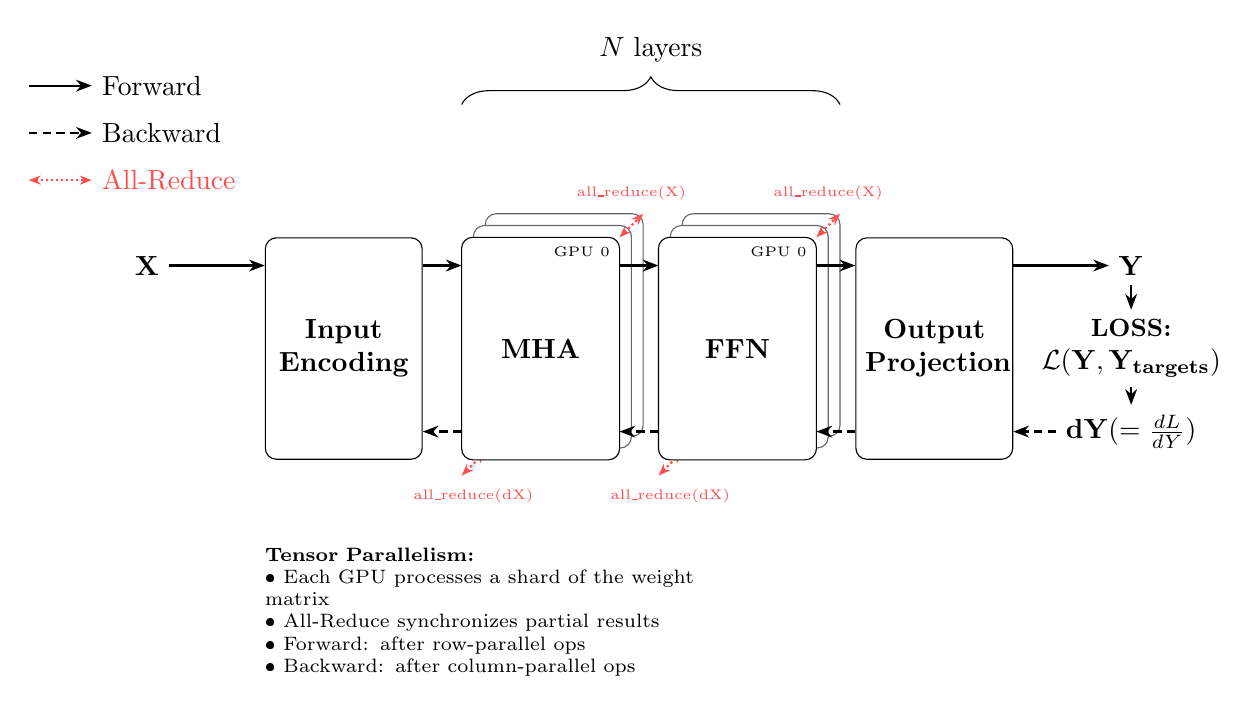
\begin{tikzpicture}[
    node distance=2.5cm,
    >=stealth,
    block/.style={rectangle, draw=black, fill=white, text width=5em, text centered, rounded corners, minimum height=8em, font=\bfseries},
    blockstack/.style={rectangle, draw=black!60, fill=white, text width=5em, text centered, rounded corners, minimum height=8em},
    forward/.style={-{Stealth[length=2mm]}, thick, black},
    backward/.style={-{Stealth[length=2mm]}, thick, black, densely dashed},
    allreduce/.style={{Stealth[length=1.5mm]}-{Stealth[length=1.5mm]}, thick, red!70, densely dotted},
    io/.style={text centered, font=\bfseries}
]
    % Title
    % \node[font=\Large\bfseries] at (10, 6) {Transformer Overall Flow (TP with 3 GPUs)};

    % Forward path nodes (horizontal)
    \node (input) [io] {$\mathbf{X}$};
    \node (encoding) [block, right of=input, yshift=-3em] {Input\\Encoding};

    % MHA blocks (3 stacked) - GPU 2 (back)
    \node (mha3) [blockstack, right of=encoding, xshift=0.3cm, yshift=0.3cm] {};
    % MHA blocks (3 stacked) - GPU 1 (middle)
    \node (mha2) [blockstack, right of=encoding, xshift=0.15cm, yshift=0.15cm] {};
    % MHA blocks (3 stacked) - GPU 0 (front)
    \node (mha) [block, right of=encoding] {MHA};

    % Small GPU labels for MHA
    \node[font=\tiny, anchor=north east] at (mha.north east) {GPU 0};

    % FFN blocks (3 stacked) - GPU 2 (back)
    \node (mlp3) [blockstack, right of=mha, xshift=0.3cm, yshift=0.3cm] {};
    % FFN blocks (3 stacked) - GPU 1 (middle)
    \node (mlp2) [blockstack, right of=mha, xshift=0.15cm, yshift=0.15cm] {};
    % FFN blocks (3 stacked) - GPU 0 (front)
    \node (mlp) [block, right of=mha] {FFN};

    % Small GPU labels for FFN
    \node[font=\tiny, anchor=north east] at (mlp.north east) {GPU 0};

    \node (output) [block, right of=mlp] {Output\\Projection};
    \node (pred) [io, right of=output, yshift=3em] {$\mathbf{Y}$};
    \node (loss) [align=center, io, right of=output] {\small LOSS:\\$\mathcal{L}(\mathbf{Y,Y_\text{targets}})$};
    \node (gradient) [io, right of=output, yshift=-3em] {$\mathbf{dY}(=\frac{dL}{dY})$};

    % All-Reduce arrows (Backward drawn first, then blocks, then Forward on top)
    % Backward All-Reduce - FFN (left-bottom corner, lower position)
    \draw [allreduce] ([yshift=-0.2cm]mlp.south west) -- ([xshift=0.3cm, yshift=0.1cm]mlp.south west);
    \node[font=\tiny, red!70, anchor=north] at ([xshift=0.15cm, yshift=-0.25cm]mlp.south west) {all\_reduce(dX)};

    % Backward All-Reduce - MHA (left-bottom corner, lower position)
    \draw [allreduce] ([yshift=-0.2cm]mha.south west) -- ([xshift=0.3cm, yshift=0.1cm]mha.south west);
    \node[font=\tiny, red!70, anchor=north] at ([xshift=0.15cm, yshift=-0.25cm]mha.south west) {all\_reduce(dX)};

    % Redraw blocks to cover backward All-Reduce arrows
    \draw [draw=black!60, fill=white, rounded corners] (mha3.south west) rectangle (mha3.north east);
    \draw [draw=black!60, fill=white, rounded corners] (mha2.south west) rectangle (mha2.north east);
    \draw [draw=black, fill=white, rounded corners, line width=0.4pt] (mha.south west) rectangle (mha.north east);
    \node[font=\bfseries] at (mha.center) {MHA};
    \node[font=\tiny, anchor=north east] at (mha.north east) {GPU 0};

    \draw [draw=black!60, fill=white, rounded corners] (mlp3.south west) rectangle (mlp3.north east);
    \draw [draw=black!60, fill=white, rounded corners] (mlp2.south west) rectangle (mlp2.north east);
    \draw [draw=black, fill=white, rounded corners, line width=0.4pt] (mlp.south west) rectangle (mlp.north east);
    \node[font=\bfseries] at (mlp.center) {FFN};
    \node[font=\tiny, anchor=north east] at (mlp.north east) {GPU 0};

    % Forward All-Reduce - MHA (right-top corner) - drawn after blocks to appear on top
    \draw [allreduce] (mha.north east) -- ([xshift=0.3cm, yshift=0.3cm]mha.north east);
    \node[font=\tiny, red!70, anchor=south] at ([xshift=0.15cm, yshift=0.35cm]mha.north east) {all\_reduce(X)};

    % Forward All-Reduce - FFN (right-top corner) - drawn after blocks to appear on top
    \draw [allreduce] (mlp.north east) -- ([xshift=0.3cm, yshift=0.3cm]mlp.north east);
    \node[font=\tiny, red!70, anchor=south] at ([xshift=0.15cm, yshift=0.35cm]mlp.north east) {all\_reduce(X)};

    % Forward arrows (upper part of blocks)
    \draw [forward] (input) -- ([yshift=3em]encoding.west);
    \draw [forward] ([yshift=3em]encoding.east) -- ([yshift=3em]mha.west);
    \draw [forward] ([yshift=3em]mha.east) -- ([yshift=3em]mlp.west);
    \draw [forward] ([yshift=3em]mlp.east) -- ([yshift=3em]output.west);
    \draw [forward] ([yshift=3em]output.east) -- (pred);
    \draw [forward] (pred) -- (loss);
    \draw [backward] (loss) -- (gradient);

    % Backward arrows (lower part of blocks)
    \draw [backward] (gradient) -- ([yshift=-3em]output.east);
    \draw [backward] ([yshift=-3em]output.west) -- ([yshift=-3em]mlp.east);
    \draw [backward] ([yshift=-3em]mlp.west) -- ([yshift=-3em]mha.east);
    \draw [backward] ([yshift=-3em]mha.west) -- ([yshift=-3em]encoding.east);

    % Brace for layer repetition (horizontal - using mlp with x offset to match mlp3)
    \draw[decorate, decoration={brace, amplitude=10pt}]
        ([yshift=4.8em]mha.north west) -- ([xshift=0.3cm, yshift=4.8em]mlp.north east)
        node[midway, above=12pt, font=\normalsize] {$N$ layers};

    % Labels (Legend)
    \coordinate (legend) at ([xshift=-1.5cm, yshift=6.5em]input);
    \draw[forward] (legend) -- ++(0.8,0) node[right, font=\normalsize] {Forward};
    \draw[backward] ([yshift=-0.6cm]legend) -- ++(0.8,0) node[right, font=\normalsize] {Backward};
    \draw[allreduce] ([yshift=-1.2cm]legend) -- ++(0.8,0) node[right, font=\normalsize] {All-Reduce};

    % TP explanation
    \node[font=\scriptsize, align=left, text width=6cm] at ([xshift=2cm, yshift=-5.5em]encoding.south) {
        \textbf{Tensor Parallelism:}\\
        • Each GPU processes a shard of the weight matrix\\
        • All-Reduce synchronizes partial results\\
        • Forward: after row-parallel ops\\
        • Backward: after column-parallel ops
    };

\end{tikzpicture}%
}

\clearpage

\subsection{MHA with Tensor Parallelism}

\subsubsection{Forward Pass}

\begin{landscape}
\thispagestyle{fancy}
\resizebox{\linewidth}{!}{%
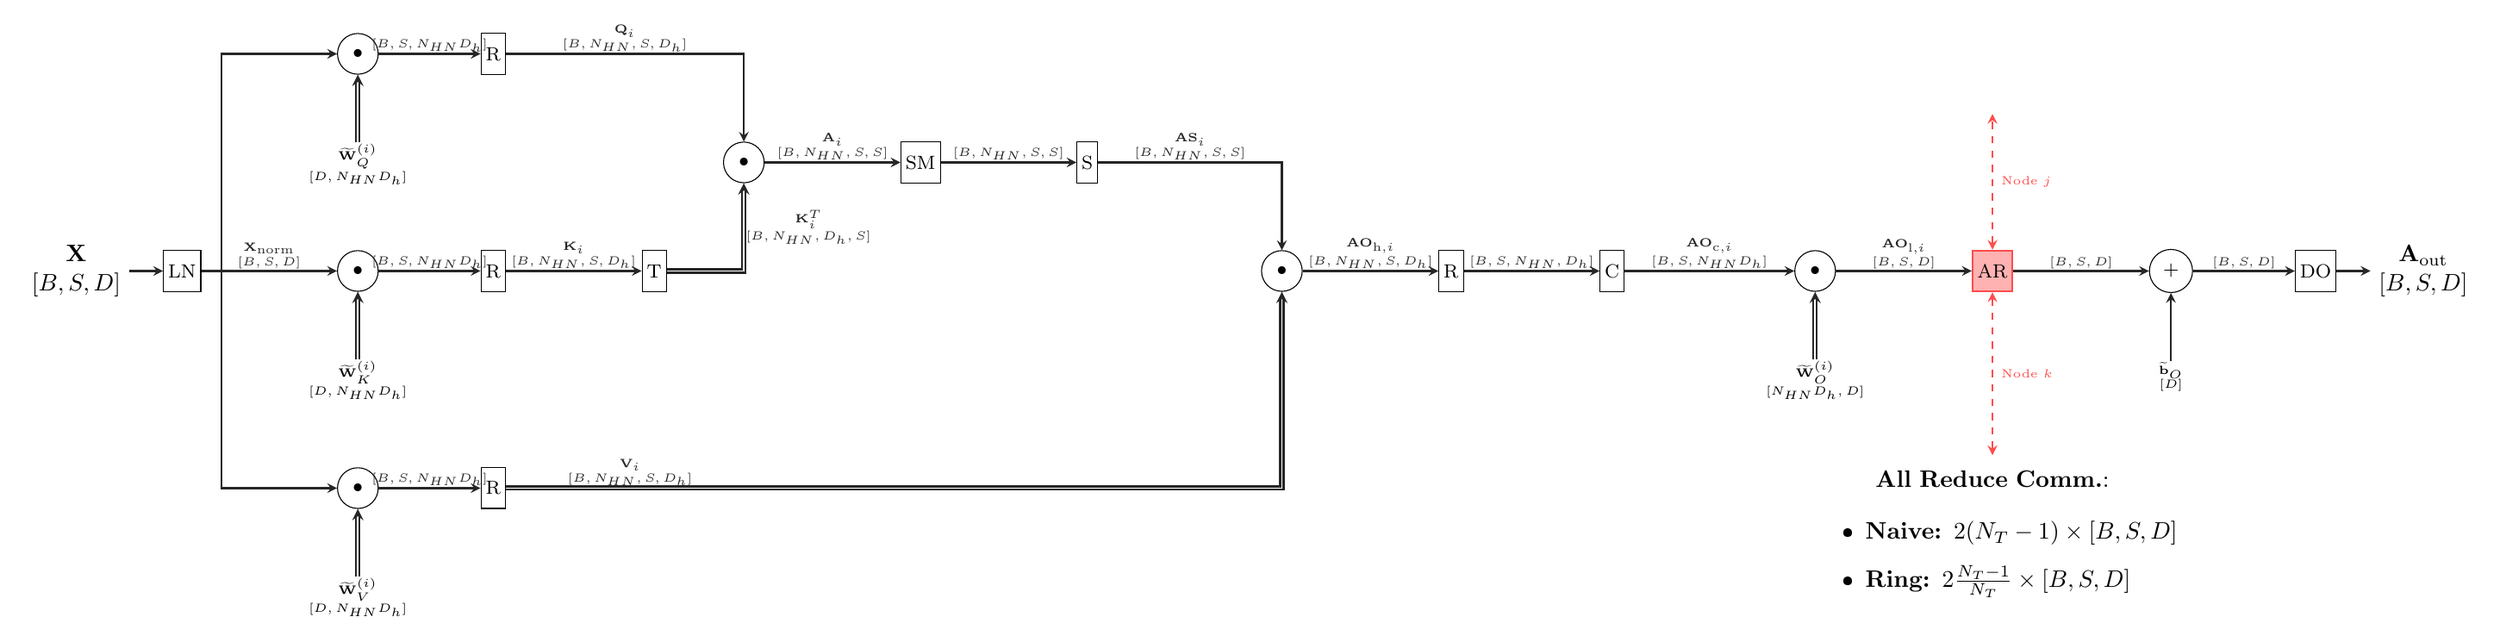
\begin{tikzpicture}[
  every node/.style={transform shape},
  >=stealth,
  auxnode/.style={draw, rectangle, fill=white, minimum height=6mm, inner sep=2pt, font=\footnotesize, align=center},
  mulnode/.style={draw, circle, fill=white, minimum size=6mm, font=\footnotesize, align=center},
  addnode/.style={draw, circle, fill=white, minimum size=6mm, font=\footnotesize, align=center},
  allreduce/.style={draw, rectangle, fill=red!30, minimum height=6mm, inner sep=2pt, font=\footnotesize, align=center, thick, draw=red!70},
  flow/.style={->, thick, black!85},
  flow2/.style={->, double, thick, black!85},
  commflow/.style={<->, thick, red!70, dashed},
  dimlabel/.style={font=\tiny, inner sep=0.5pt, align=center}
]
% \node[font=\Large\bfseries] at (9, 4.5) {Multi-Head Attention Forward Pass (Node $i$)};

\node (Input) at (0.5, 0) [align=center] {$\mathbf{X}$\\$[B,S,D]$};
\node[auxnode] (LN) [right=0.5cm of Input] {LN};

\node[mulnode] (Proj_Q) [right=2.0cm of LN, yshift=3.2cm] {$\bullet$};
\node[auxnode] (R_Q) [right=1.5cm of Proj_Q] {R};

\node[mulnode] (Proj_K) [right=2.0cm of LN, yshift=0cm] {$\bullet$};
\node[auxnode] (R_K) [right=1.5cm of Proj_K] {R};

\node[mulnode] (Proj_V) [right=2.0cm of LN, yshift=-3.2cm] {$\bullet$};
\node[auxnode] (R_V) [right=1.5cm of Proj_V] {R};

\node[dimlabel] (WQ) [align=center, below=1.0cm of Proj_Q] {$\widetilde{\mathbf{W}}_{Q}^{(i)}$\\$[D,N_{HN}D_h]$};
\node[dimlabel] (WK) [align=center, below=1.0cm of Proj_K] {$\widetilde{\mathbf{W}}_{K}^{(i)}$\\$[D,N_{HN}D_h]$};
\node[dimlabel] (WV) [align=center, below=1.0cm of Proj_V] {$\widetilde{\mathbf{W}}_{V}^{(i)}$\\$[D,N_{HN}D_h]$};

\node[auxnode] (T_K) [right=2.0cm of R_K] {T};
\node[mulnode] (QK) [right=3.2cm of R_Q, yshift=-1.6cm] {$\bullet$};
\node[auxnode] (SM) [right=2.0cm of QK] {SM};
\node[auxnode] (Soft) [right=2.0cm of SM] {S};
\node[mulnode] (PV) [right=2.4cm of Soft, yshift=-1.6cm] {$\bullet$};

\node[auxnode] (R_Merge) [right=2.0cm of PV] {R};
\node[auxnode] (Cat) [right=2.0cm of R_Merge] {C};

\node[mulnode] (OProj) [right=2.5cm of Cat] {$\bullet$};
\node[dimlabel] (WO_FWD) [align=center, below=1.0cm of OProj] {$\widetilde{\mathbf{W}}_{O}^{(i)}$\\$[N_{HN}D_h,D]$};
\node[allreduce] (AR) [right=2.0cm of OProj] {AR};
\node[
  align=center,
  below=2.5cm of AR,
  text width=5.5cm % 적당한 값으로 조정
] (AR_info) {%
  \textbf{All Reduce Comm.}:\\[2pt]
  \begin{itemize}
    \item \textbf{Naive:} $2(N_T-1) \times [B,S,D]$
    \item \textbf{Ring:} $2\frac{N_T-1}{N_T} \times [B,S,D]$
  \end{itemize}
};
\node[addnode] (AddB) [right=2.0cm of AR] {+};
\node[dimlabel] (BO) [align=center, below=1.0cm of AddB] {$\widetilde{\mathbf{b}}_{O}$\\$[D]$};
\node[auxnode] (Drop) [right=1.5cm of AddB] {DO};
\node (Aout) [align=center, right=0.5cm of Drop] {$\mathbf{A}_{\text{out}}$\\$[B,S,D]$};

\draw[flow] (Input) -- (LN);

\draw[flow] (LN.east) -- ++(0.3,0) |- (Proj_Q.west);
\draw[flow] (LN) -- (Proj_K.west) node[dimlabel, midway, above]{$\mathbf{X}_{\text{norm}}$\\$[B,S,D]$};
\draw[flow] (LN.east) -- ++(0.3,0) |- (Proj_V.west);

\draw[flow2] (WQ) -- (Proj_Q);
\draw[flow2] (WK) -- (Proj_K);
\draw[flow2] (WV) -- (Proj_V);

\draw[flow] (Proj_Q) -- (R_Q) node[dimlabel, midway, above]{$[B,S,N_{HN}D_h]$};
\draw[flow] (Proj_K) -- (R_K) node[dimlabel, midway, above]{$[B,S,N_{HN}D_h]$};
\draw[flow] (Proj_V) -- (R_V) node[dimlabel, midway, above]{$[B,S,N_{HN}D_h]$};

\draw[flow] (R_Q) -| (QK) node[dimlabel, near start, above]{$\mathbf{Q}_i$\\$[B,N_{HN},S,D_h]$};
\draw[flow] (R_K) -- (T_K) node[dimlabel, midway, above]{$\mathbf{K}_i$\\$[B,N_{HN},S,D_h]$};
\draw[flow2] (T_K) -| (QK) node[dimlabel, near end, right]{$\mathbf{K}_i^{T}$\\$[B,N_{HN},D_h,S]$};

\draw[flow] (QK) -- (SM) node[dimlabel, midway, above]{$\mathbf{A}_i$\\$[B,N_{HN},S,S]$};
\draw[flow] (SM) -- (Soft) node[dimlabel, midway, above]{$[B,N_{HN},S,S]$};
\draw[flow] (Soft) -| (PV) node[dimlabel, near start, above]{$\mathbf{AS}_i$\\$[B,N_{HN},S,S]$};
\draw[flow2] (R_V) -| (PV) node[dimlabel, pos=0.08, above]{$\mathbf{V}_i$\\$[B,N_{HN},S,D_h]$};

\draw[flow] (PV) -- (R_Merge) node[dimlabel, midway, above]{$\mathbf{AO}_{\text{h},i}$\\$[B,N_{HN},S,D_h]$};
\draw[flow] (R_Merge) -- (Cat) node[dimlabel, midway, above]{$[B,S,N_{HN},D_h]$};
\draw[flow] (Cat) -- (OProj) node[dimlabel, midway, above]{$\mathbf{AO}_{\text{c},i}$\\$[B,S,N_{HN}D_h]$};
\draw[flow2] (WO_FWD) -- (OProj);
\draw[flow] (OProj) -- (AR) node[dimlabel, midway, above]{$\mathbf{AO}_{\text{l},i}$\\$[B,S,D]$};

% All-Reduce communication arrows
\draw[commflow] (AR.north) -- ++(0, 2.0) node[midway, right, font=\tiny]{Node $j$};
\draw[commflow] (AR.south) -- ++(0, -2.4) node[midway, right, font=\tiny]{Node $k$};

\draw[flow] (AR) -- (AddB) node[dimlabel, midway, above]{$[B,S,D]$};
\draw[flow] (BO) -- (AddB);
\draw[flow] (AddB) -- (Drop) node[dimlabel, midway, above]{$[B,S,D]$};
\draw[flow] (Drop) -- (Aout);
\end{tikzpicture}%
}
\end{landscape}
\clearpage

\subsubsection{Backward Pass}

\begin{landscape}
\thispagestyle{fancy}
\par\vspace{1cm}
\noindent
\resizebox{\linewidth}{!}{%
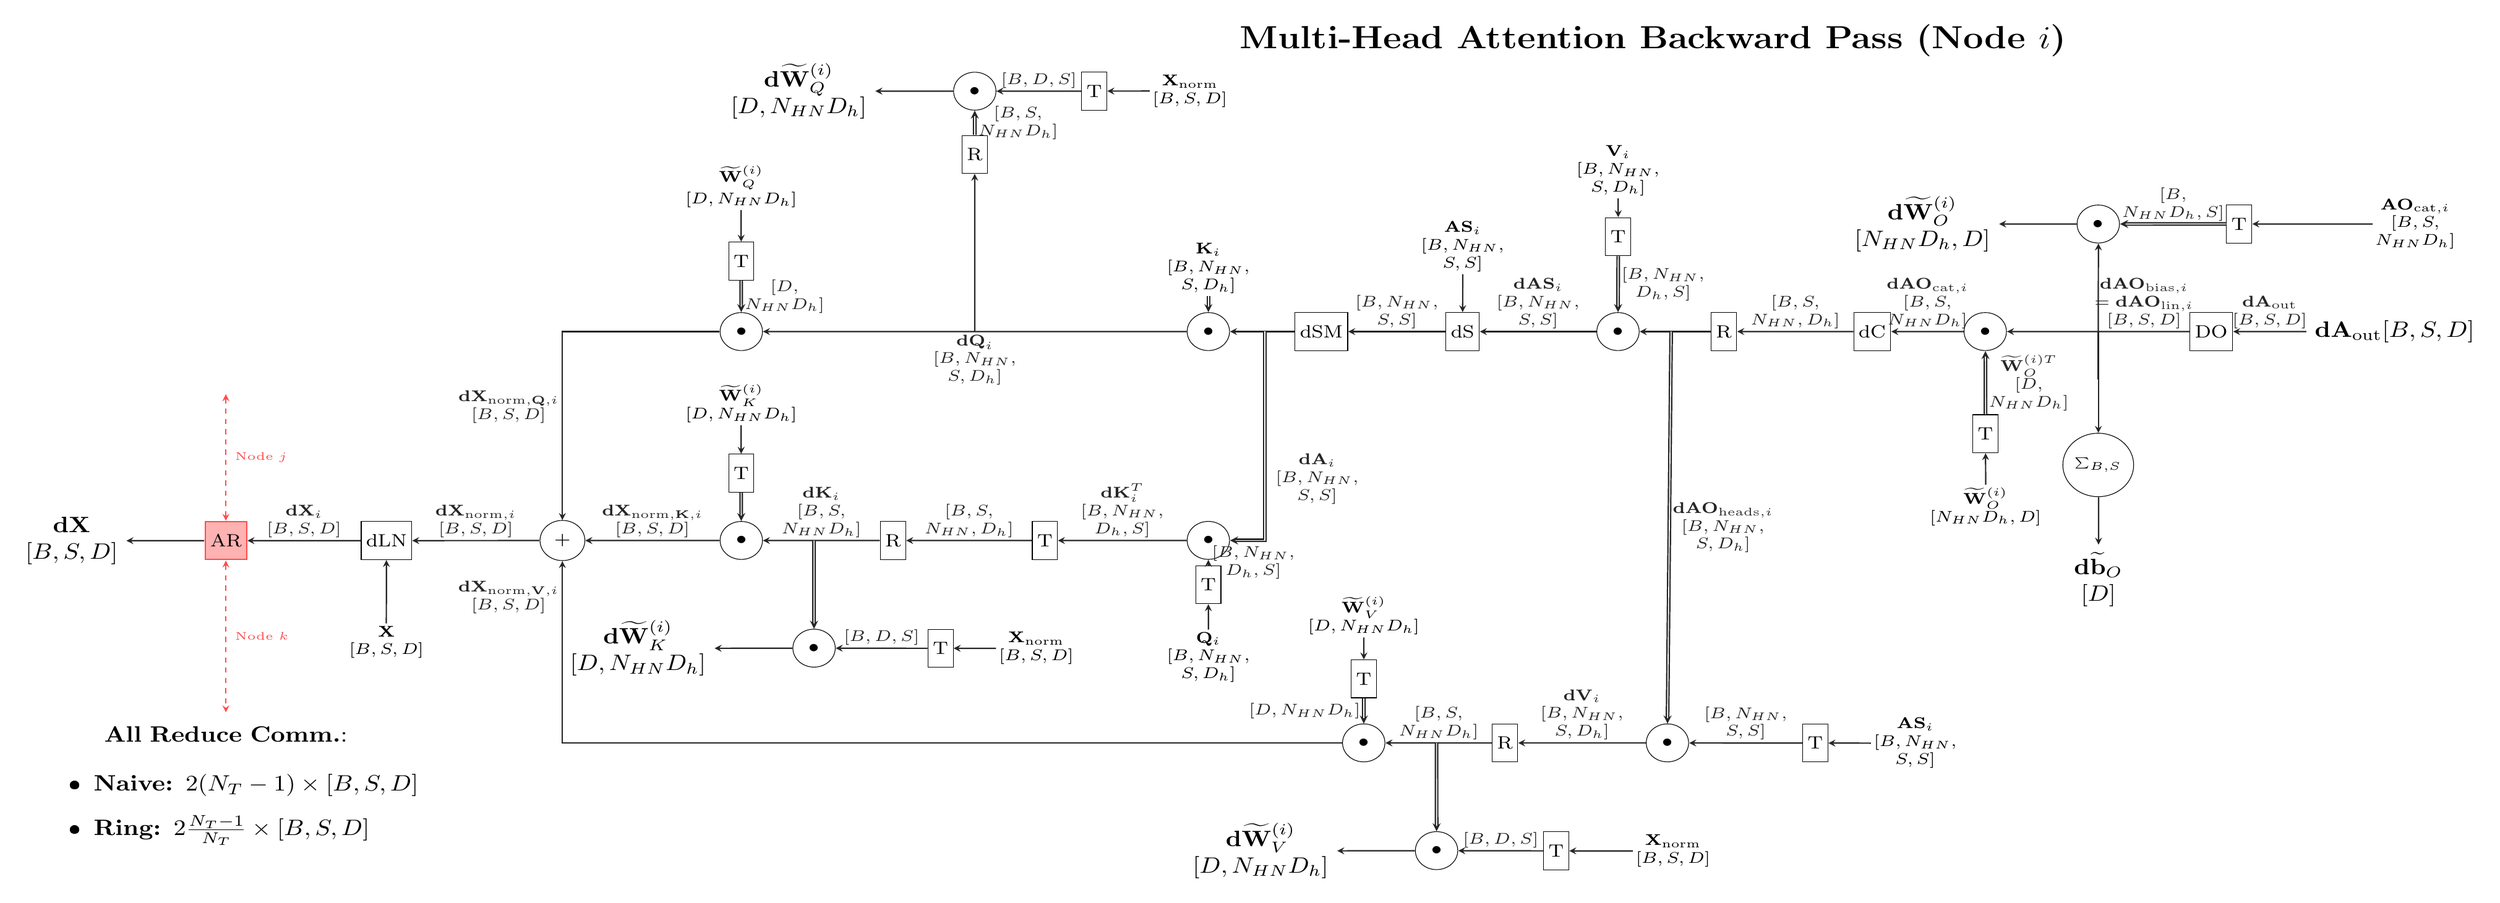
\begin{tikzpicture}[
  every node/.style={transform shape},
  >=stealth,
  auxnode/.style={draw, rectangle, fill=white, minimum height=6mm, inner sep=2pt, font=\footnotesize, align=center},
  mulnode/.style={draw, circle, fill=white, minimum size=6mm, font=\footnotesize, align=center},
  addnode/.style={draw, circle, fill=white, minimum size=6mm, font=\footnotesize, align=center},
  sumnode/.style={draw, circle, fill=white, minimum size=6mm, font=\tiny, align=center},
  allreduce/.style={draw, rectangle, fill=red!30, minimum height=6mm, inner sep=2pt, font=\footnotesize, align=center, thick, draw=red!70},
  flow/.style={->, thick, black!85},
  flow2/.style={->, double, thick, black!85},
  commflow/.style={<->, thick, red!70, dashed},
  dimlabel/.style={font=\scriptsize, inner sep=1pt, align=center},
  gradflow/.style={->, thick, black!85},
  gradweight/.style={->, thick, black!85}
]

\begin{scope}[xscale=1.45, yscale=1.3]

\def\yoffset{-1.0}
\def\dVXyoffset{-6.5}

\coordinate (Grad_Aout_B) at (17.5, \yoffset);
\coordinate (dDrop_center) at (15.9, \yoffset);
\coordinate (ProjGradSplit) at (14.3, \yoffset);
\coordinate (dOProj_center) at (12.7, \yoffset);
\coordinate (C_center) at (11.1, \yoffset);
\coordinate (R_center) at (9.0, \yoffset);
\coordinate (dPV_AS_calc_center) at (7.5, \yoffset);
\coordinate (dSoft_center) at (5.3, \yoffset);
\coordinate (dSM_calc_center) at (3.3, \yoffset);
\coordinate (dV_calc_center) at (8.2, \dVXyoffset+\yoffset);
\coordinate (R_V_bwd_center) at (5.9, \dVXyoffset+\yoffset);
\coordinate (dVX_calc_center) at (3.9, \dVXyoffset+\yoffset);
\coordinate (dQK_calc_Q_center) at (1.7, \yoffset);
\coordinate (dQK_calc_K_center) at (1.7, -3.3+\yoffset);
\coordinate (K_BWD_input_center) at (1.7, 1.0+\yoffset);
\coordinate (T_Q_bwd_center) at (1.7, -4.0+\yoffset);

\node[font=\Large\bfseries] at (8, 4.6+\yoffset) {Multi-Head Attention Backward Pass (Node $i$)};

\node (Grad_Aout_B) at (18.5, \yoffset) {$\mathbf{dA}_{\text{out}}$\\$[B,S,D]$};
\node[auxnode] (DO) at (dDrop_center) {DO};
\node[mulnode] (dOProj) at (dOProj_center) {$\bullet$};

\node[auxnode] (T_WO) [below=1.0cm of dOProj] {T};
\node[dimlabel] (WO_BWD) [below=0.5cm of T_WO] {$\widetilde{\mathbf{W}}_{O}^{(i)}$\\$[N_{HN}D_h,D]$};

\node[mulnode] (dWO_calc) at ($(ProjGradSplit)+(0, 1.7)$) {$\bullet$};
\node[align=center, left=1.1cm of dWO_calc]
  (dWO_GRAD) {$\mathbf{d}\widetilde{\mathbf{W}}_{O}^{(i)}$\\$[N_{HN}D_h,D]$};
\node[auxnode] (T_AO_in) [right=1.5cm of dWO_calc] {T};
\node[dimlabel] (AO_in_local_label) [right=1.7cm of T_AO_in] {$\mathbf{AO}_{\text{cat},i}$\\$[B,S,$\\$N_{HN}D_h]$};

\node[auxnode] (C) at (C_center) {dC};
\node[auxnode] (R) at (R_center) {R};

\node[mulnode] (dPV_AS_calc) at (dPV_AS_calc_center) {$\bullet$};
\node[auxnode] (dSoft) at (dSoft_center) {dS};
\node[auxnode] (dSM_calc) at (dSM_calc_center) {dSM};

\node[mulnode] (dQK_calc_Q) at (dQK_calc_Q_center) {$\bullet$};
\node[mulnode] (dQX_proj_calc) [left=6.0cm of dQK_calc_Q] {$\bullet$};

\node[mulnode] (dQK_calc_K) at (dQK_calc_K_center) {$\bullet$};
\node[mulnode] (dKX_proj_calc) [left=6.0cm of dQK_calc_K] {$\bullet$};

\node[dimlabel] (K_BWD_input) at (K_BWD_input_center) {$\mathbf{K}_i$\\$[B,N_{HN},$\\$S,D_h]$};
\node[auxnode] (T_Q_bwd) at (T_Q_bwd_center) {T};
\node[dimlabel] (Q_BWD_input) [below=0.4cm of T_Q_bwd] {$\mathbf{Q}_i$\\$[B,N_{HN},$\\$S,D_h]$};

\node[dimlabel] (V_FWD) [above=1.8cm of dPV_AS_calc] {$\mathbf{V}_i$\\$[B,N_{HN},$\\$S,D_h]$};
\node[auxnode] (T_V_bwd) [below=0.3cm of V_FWD] {T};

\node[mulnode] (dV_calc) at (dV_calc_center) {$\bullet$};
\node[auxnode] (T_AS_bwd) [right=1.6cm of dV_calc] {T};
\node[dimlabel] (AS_BWD_for_V) [right=0.6cm of T_AS_bwd] {$\mathbf{AS}_i$\\$[B,N_{HN},$\\$S,S]$};

\node[auxnode] (R_V_bwd) at (R_V_bwd_center) {R};
\node[mulnode] (dVX_calc) at (dVX_calc_center) {$\bullet$};

\node[auxnode] (T_WV) [above=0.4cm of dVX_calc] {T};
\node[dimlabel] (WV_BWD) [above=0.35cm of T_WV] {$\widetilde{\mathbf{W}}_{V}^{(i)}$\\$[D,N_{HN}D_h]$};

\node[sumnode] (Sum_dBO) [below=1.6cm of ProjGradSplit] {$\sum_{B, S}$};
\node (dBO) [align=center, below=0.75cm of Sum_dBO] {$\mathbf{d}\widetilde{\mathbf{b}}_{O}$\\$[D]$};

\draw[gradflow] (Grad_Aout_B) -- (DO)
  node[dimlabel, midway, above]{$\mathbf{dA}_{\text{out}}$\\$[B,S,D]$};

\draw[gradflow] (DO) -- (dOProj)
  node[dimlabel, pos=0.25, above]{$\mathbf{dAO}_{\text{bias},i}$\\$=\mathbf{dAO}_{\text{lin},i}$\\$[B,S,D]$};

\draw[gradflow] (ProjGradSplit) -- (dWO_calc.south);
\draw[gradflow] (ProjGradSplit) -- ([yshift=-0.75cm]ProjGradSplit) -| (Sum_dBO.north);

\draw[gradflow] (dOProj) -- (C)
  node[dimlabel, midway, above]{$\mathbf{dAO}_{\text{cat},i}$\\$[B,S,$\\$N_{HN}D_h]$};
\draw[gradflow] (C) -- (R)
  node[dimlabel, midway, above]{$[B,S,$\\$N_{HN},D_h]$};

\coordinate (R_split_point) at ($(dPV_AS_calc)!0.5!(R)$);
\draw[gradflow] (R.west) -- (dPV_AS_calc.east);
\draw[flow2] (R_split_point) -- (dV_calc.north)
  node[dimlabel, midway, right]{$\mathbf{dAO}_{\text{heads},i}$\\$[B,N_{HN},$\\$S,D_h]$};

\draw[gradflow] (V_FWD.south) -- (T_V_bwd.north);
\draw[flow2] (T_V_bwd.south) -- (dPV_AS_calc.north)
  node[dimlabel, midway, right]{$[B,N_{HN},$\\$D_h,S]$};
\draw[gradflow] (dPV_AS_calc.west) -- (dSoft.east)
  node[dimlabel, midway, above]{$\mathbf{dAS}_i$\\$[B,N_{HN},$\\$S,S]$};

\node (AS_BWD_dS) [dimlabel, above=0.6cm of dSoft] {$\mathbf{AS}_i$\\$[B,N_{HN},$\\$S,S]$};
\draw[gradflow] (AS_BWD_dS.south) -- (dSoft.north);
\draw[gradflow] (dSoft.west) -- (dSM_calc.east)
  node[dimlabel, midway, above]{$[B,N_{HN},$\\$S,S]$};

\coordinate (dA_Split_X) at ($(dSM_calc_center)!0.5!(dQK_calc_Q_center)$);
\coordinate (dA_Split) at (dA_Split_X |- dQK_calc_Q.east);
\draw[gradflow] (dSM_calc.west) -- (dQK_calc_Q.east);
\draw[flow2] (dA_Split) -- (dA_Split |- dQK_calc_K.east) -- (dQK_calc_K.east)
  node[dimlabel, pos=-1.5, above, yshift=15]{$\mathbf{dA}_i$\\$[B,N_{HN},$\\$S,S]$};

\draw[flow2] (K_BWD_input.south) -- (dQK_calc_Q.north);
\draw[gradweight] (dQK_calc_Q) -- (dQX_proj_calc)
  node[dimlabel, midway, below]{$\mathbf{dQ}_i$\\$[B,N_{HN},$\\$S,D_h]$};

\node[auxnode] (T_WQ_bwd) [above=0.5cm of dQX_proj_calc] {T};
\node[dimlabel] (WQ_bwd) [above=0.5cm of T_WQ_bwd] {$\widetilde{\mathbf{W}}_{Q}^{(i)}$\\$[D,N_{HN}D_h]$};
\draw[flow] (WQ_bwd) -- (T_WQ_bwd);
\draw[flow2] (T_WQ_bwd.south) -- (dQX_proj_calc.north)
  node[dimlabel, midway, right]{$[D,$\\$N_{HN}D_h]$};

\draw[flow] (Q_BWD_input.north) -- (T_Q_bwd.south);
\draw[flow] (T_Q_bwd.north) -- (dQK_calc_K.south)
  node[dimlabel, pos=0.55, right]{$[B,N_{HN},$\\$D_h,S]$};

\node[auxnode] (T_dK) at ($(dQK_calc_K)!0.35!(dKX_proj_calc)$) {T};
\node[auxnode] (R_dK_mid) at ($(T_dK)!0.5!(dKX_proj_calc)$) {R};

\draw[gradweight] (dQK_calc_K) -- (T_dK)
  node[dimlabel, midway, above]{$\mathbf{dK}_i^T$\\$[B,N_{HN},$\\$D_h,S]$};
\draw[gradweight] (T_dK) -- (R_dK_mid)
  node[dimlabel, midway, above]{$[B,S,$\\$N_{HN},D_h]$};
\draw[gradweight] (R_dK_mid) -- (dKX_proj_calc)
  node[dimlabel, midway, above]{$\mathbf{dK}_i$\\$[B,S,$\\$N_{HN}D_h]$};

\node[auxnode] (T_WK_bwd) [above=0.45cm of dKX_proj_calc] {T};
\node[dimlabel] (WK_bwd) [above=0.45cm of T_WK_bwd] {$\widetilde{\mathbf{W}}_{K}^{(i)}$\\$[D,N_{HN}D_h]$};
\draw[gradflow] (WK_bwd) -- (T_WK_bwd);
\draw[flow2] (T_WK_bwd.south) -- (dKX_proj_calc.north);

\draw[gradflow] (AS_BWD_for_V.west) -- (T_AS_bwd.east);
\draw[gradflow] (T_AS_bwd.west) -- (dV_calc.east)
  node[dimlabel, midway, above]{$[B,N_{HN},$\\$S,S]$};
\draw[gradflow] (dV_calc.west) -- (R_V_bwd.east)
  node[dimlabel, midway, above]{$\mathbf{dV}_i$\\$[B,N_{HN},$\\$S,D_h]$};
\draw[gradflow] (R_V_bwd) -- (dVX_calc.east)
  node[dimlabel, midway, above]{$[B,S,$\\$N_{HN}D_h]$};

\draw[gradflow] (WV_BWD) -- (T_WV);
\draw[flow2] (T_WV) -- (dVX_calc.north)
  node[dimlabel, midway, left]{$[D,N_{HN}D_h]$};

\node[addnode] (Sum_dXnorm) [left=1.9cm of dKX_proj_calc] {$+$};

\draw[gradweight] (dQX_proj_calc.west) -| node[dimlabel, pos=0.7, left]{$\mathbf{dX}_{\text{norm},\mathbf{Q},i}$\\$[B,S,D]$} (Sum_dXnorm.north);
\draw[gradweight] (dKX_proj_calc.west) -- node[dimlabel, midway, above]{$\mathbf{dX}_{\text{norm},\mathbf{K},i}$\\$[B,S,D]$} (Sum_dXnorm.east);
\draw[gradweight] (dVX_calc.west) -| node[dimlabel, pos=0.9, left]{$\mathbf{dX}_{\text{norm},\mathbf{V},i}$\\$[B,S,D]$} (Sum_dXnorm.south);

\coordinate (dV_branch) at ($(R_V_bwd.west)!0.52!(dVX_calc.east)$);
\node[mulnode] (dWV_mul) at ($(dV_branch)+(0,-1.7cm)$) {$\bullet$};
\draw[flow2] (dV_branch) -- (dWV_mul.north);

\node[auxnode] (T_Xnorm) [right=1.2cm of dWV_mul] {T};
\node[dimlabel] (Xnorm_local) [right=0.9cm of T_Xnorm] {$\mathbf{X}_{\text{norm}}$\\$[B,S,D]$};
\draw[gradflow] (Xnorm_local) -- (T_Xnorm);
\draw[gradflow] (T_Xnorm.west) -- (dWV_mul.east)
  node[dimlabel, midway, above]{$[B,D,S]$};
\node (dWV_out) [align=center, left=1.1cm of dWV_mul] {$\mathbf{d}\widetilde{\mathbf{W}}_{V}^{(i)}$\\$[D,N_{HN}D_h]$};
\draw[gradweight] (dWV_mul.west) -- (dWV_out);

\coordinate (dQ_branch) at ($(dQK_calc_Q.east)!0.50!(dQX_proj_calc.west)$);
\node[mulnode] (dWQ_mul) at ($(dQ_branch)+(0,3.8cm)$) {$\bullet$};
\node[auxnode] (R_dQ_for_WQ) at ($(dWQ_mul)+(0,-1.0cm)$) {R};
\draw[gradflow]  (dQ_branch) -- (R_dQ_for_WQ.south);
\draw[flow2] (R_dQ_for_WQ.north) -- (dWQ_mul.south)
  node[dimlabel, midway, right]{$[B,S,$\\$N_{HN}D_h]$};

\node[auxnode] (T_XnormQ) [right=1.2cm of dWQ_mul] {T};
\node[dimlabel] (Xnorm_localQ) [right=0.6cm of T_XnormQ] {$\mathbf{X}_{\text{norm}}$\\$[B,S,D]$};
\draw[gradflow] (Xnorm_localQ) -- (T_XnormQ);
\draw[gradflow] (T_XnormQ.west) -- (dWQ_mul.east)
  node[dimlabel, midway, above]{$[B,D,S]$};
\node (dWQ_out) [align=center, left=1.1cm of dWQ_mul] {$\mathbf{d}\widetilde{\mathbf{W}}_{Q}^{(i)}$\\$[D,N_{HN}D_h]$};
\draw[gradweight] (dWQ_mul.west) -- (dWQ_out);

\coordinate (dK_branch) at ($(R_dK_mid)!0.52!(dKX_proj_calc)$);
\node[mulnode] (dWK_mul) at ($(dK_branch)+(0,-1.7cm)$) {$\bullet$};
\draw[flow2]  (dK_branch) -- (dWK_mul.north);

\node[auxnode] (T_XnormK) [right=1.3cm of dWK_mul] {T};
\node[dimlabel, right=0.6cm of T_XnormK] (Xnorm_localK) {$\mathbf{X}_{\text{norm}}$\\$[B,S,D]$};
\draw[gradflow] (Xnorm_localK) -- (T_XnormK);
\draw[gradflow] (T_XnormK.west) -- (dWK_mul.east)
  node[dimlabel, midway, above]{$[B,D,S]$};
\node (dWK_out) [align=center, left=1.1cm of dWK_mul] {$\mathbf{d}\widetilde{\mathbf{W}}_{K}^{(i)}$\\$[D,N_{HN}D_h]$};
\draw[gradweight] (dWK_mul.west) -- (dWK_out);

\draw[gradweight] (Sum_dBO) -- (dBO);

\draw[gradflow] (WO_BWD) -- (T_WO);
\draw[flow2] (T_WO) -- (dOProj)
  node[dimlabel, midway, right]{$\widetilde{\mathbf{W}}_{O}^{(i)T}$\\$[D,$\\$N_{HN}D_h]$};
\draw[gradflow] (AO_in_local_label) -- (T_AO_in);
\draw[flow2] (T_AO_in) -- (dWO_calc.east)
  node[dimlabel, midway, above]{$[B,$\\$N_{HN}D_h,S]$};
\draw[gradweight] (dWO_calc) -- (dWO_GRAD);

\node[auxnode] (dLN) [left=1.8cm of Sum_dXnorm] {dLN};
\draw[gradweight] (Sum_dXnorm.west) -- node[dimlabel, midway, above]
  {$\mathbf{dX}_{\text{norm},i}$\\$[B,S,D]$} (dLN.east);

\node[allreduce] (AR) [left=1.6cm of dLN] {AR};
\node[
  align=center,
  below=2.5cm of AR,
  text width=5.5cm
] (AR_info) {%
  \textbf{All Reduce Comm.}:\\[2pt]
  \begin{itemize}
    \item \textbf{Naive:} $2(N_T-1) \times [B,S,D]$
    \item \textbf{Ring:} $2\frac{N_T-1}{N_T} \times [B,S,D]$
  \end{itemize}
};

% All-Reduce communication arrows
\draw[commflow] (AR.north) -- ++(0, 2.0) node[midway, right, font=\tiny]{Node $j$};
\draw[commflow] (AR.south) -- ++(0, -2.4) node[midway, right, font=\tiny]{Node $k$};

\draw[gradweight] (dLN.west) -- (AR.east) node[dimlabel, midway, above]{$\mathbf{dX}_i$\\$[B,S,D]$};

\node (dX_OUT) [align=center, left=1.1cm of AR] {$\mathbf{dX}$\\$[B,S,D]$};
\draw[gradweight] (AR.west) -- (dX_OUT);

\node[dimlabel] (LNCache) [below=1.0cm of dLN] {$\mathbf{X}$\\$[B,S,D]$};
\draw[gradflow] (LNCache.north) -- (dLN.south);

\end{scope}
\end{tikzpicture}
}
\end{landscape}
\clearpage

\subsection{MLP with Tensor Parallelism}

\subsubsection{Forward Pass}
\resizebox{\linewidth}{!}{%
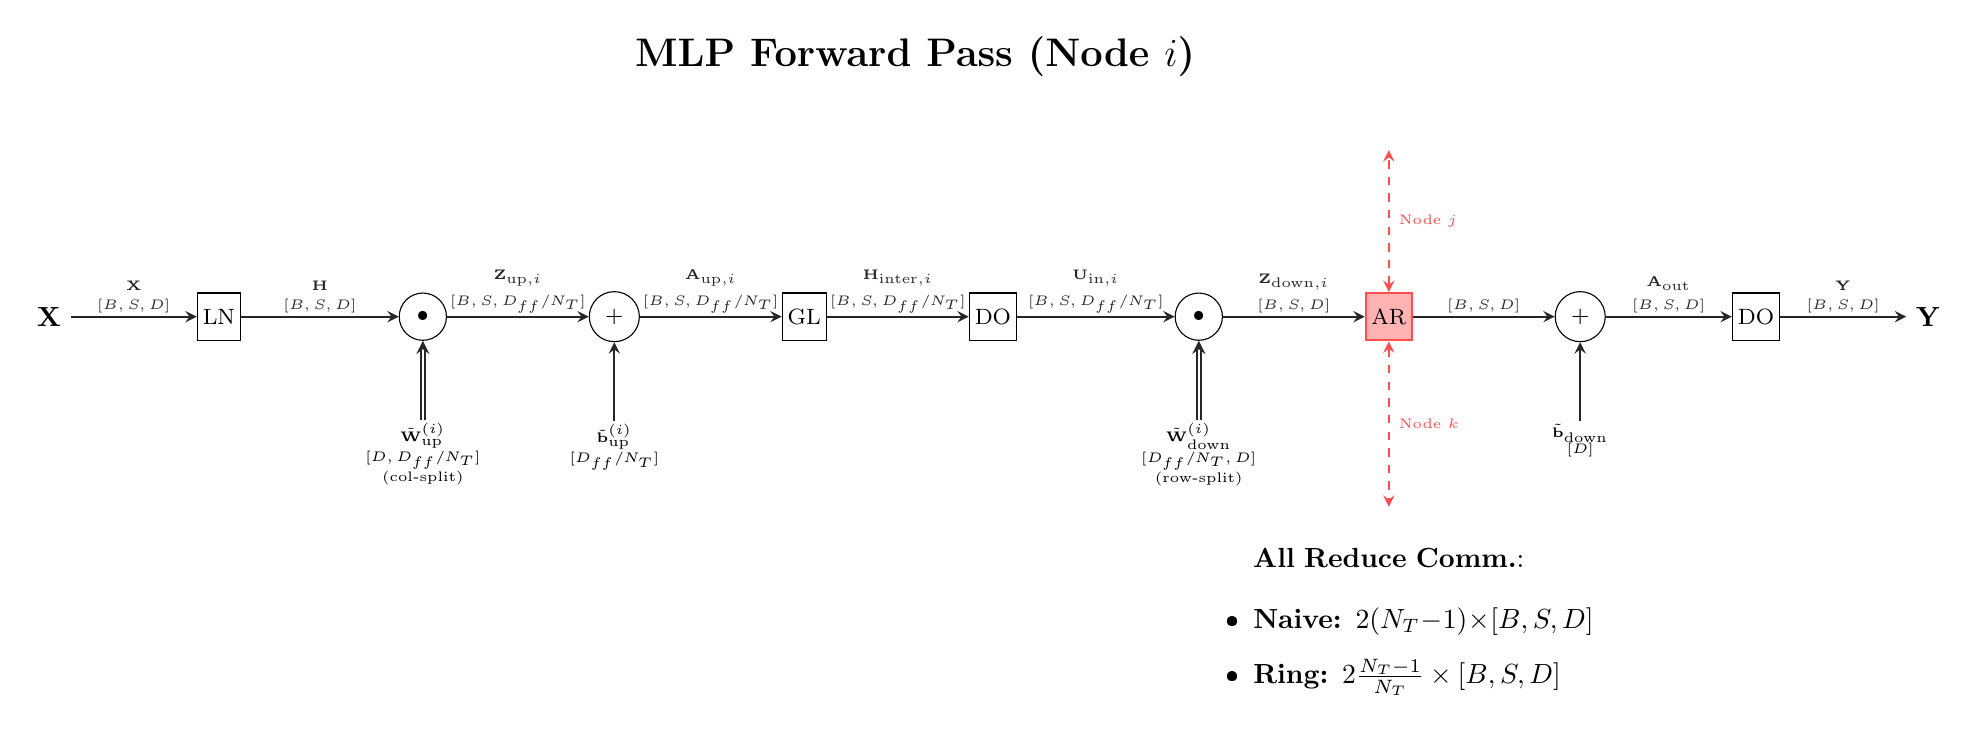
\begin{tikzpicture}[
    >=stealth,
    auxnode/.style={draw, rectangle, fill=white, minimum height=6mm, inner sep=2pt, font=\footnotesize, align=center},
    mulnode/.style={draw, circle, fill=white, minimum size=6mm, font=\footnotesize, align=center},
    addnode/.style={draw, circle, fill=white, minimum size=6mm, font=\footnotesize, align=center},
    allreduce/.style={draw, rectangle, fill=red!30, minimum height=6mm, inner sep=2pt, font=\footnotesize, align=center, thick, draw=red!70},
    sumnode/.style={draw, circle, fill=white, minimum size=6mm, font=\tiny, align=center},
    flow/.style={->, thick, black!85},
    flow2/.style={double, ->, thick, black!85},
    commflow/.style={<->, thick, red!70, dashed},
    dimlabel/.style={font=\tiny, inner sep=1pt, align=center}
]
    \node[font=\Large\bfseries] at (11, 2.8) {MLP Forward Pass (Node $i$)};

    \pgfmathsetmacro{\verticaloffset}{-0.5}

    \node            (MIn)   at (0,\verticaloffset) {$\mathbf{X}$};
    \node[auxnode]   (LN2)   [right=1.6cm of MIn] {LN};
    \node[mulnode]   (L1Mul) [right=2.0cm of LN2] {$\bullet$};
    \node[dimlabel]  (Wup)   [below=1.0cm of L1Mul] {$\tilde{\mathbf{W}}_{\text{up}}^{(i)}$\\$[D, D_{ff}/N_T]$\\(col-split)};
    \node[addnode]   (AddB1) [right=1.8cm of L1Mul] {+};
    \node[dimlabel]  (Bup)   [below=1.0cm of AddB1] {$\tilde{\mathbf{b}}_{\text{up}}^{(i)}$\\$[D_{ff}/N_T]$};
    \node[auxnode]   (Act)   [right=1.8cm of AddB1] {GL};
    \node[auxnode]   (Drop1) [right=1.8cm of Act] {DO};
    \node[mulnode]   (L2Mul) [right=2.0cm of Drop1] {$\bullet$};
    \node[dimlabel]  (Wdown) [below=1.0cm of L2Mul] {$\tilde{\mathbf{W}}_{\text{down}}^{(i)}$\\$[D_{ff}/N_T, D]$\\(row-split)};
    \node[allreduce] (AR)    [right=1.8cm of L2Mul] {AR};
    \node[
      align=center,
      below=2.5cm of AR,
      text width=5.2cm
    ] (AR_info) {%
      \textbf{All Reduce Comm.}:\\[2pt]
      \begin{itemize}
        \item \textbf{Naive:} $2(N_T-1) \times [B,S,D]$
        \item \textbf{Ring:} $2\frac{N_T-1}{N_T} \times [B,S,D]$
      \end{itemize}
    };
    \node[addnode]   (AddB2) [right=1.8cm of AR] {+};
    \node[dimlabel]  (Bdown) [below=1.0cm of AddB2] {$\tilde{\mathbf{b}}_{\text{down}}$\\$[D]$};
    \node[auxnode]   (Drop2) [right=1.6cm of AddB2] {DO};
    \node            (MOut)  [right=1.6cm of Drop2] {$\mathbf{Y}$};

    % All-Reduce communication arrows
    \draw[commflow] (AR.north) -- ++(0, 1.8) node[midway, right, font=\tiny]{Node $j$};
    \draw[commflow] (AR.south) -- ++(0, -2.1) node[midway, right, font=\tiny]{Node $k$};

    \draw[flow] (MIn) -- (LN2) node[dimlabel, midway, above]{\shortstack{$\mathbf{X}$\\$[B,S,D]$}};
    \draw[flow] (LN2) -- (L1Mul) node[dimlabel, midway, above]{\shortstack{$\mathbf{H}$\\$[B,S,D]$}};
    \draw[flow2] (Wup) -- (L1Mul);
    \draw[flow] (L1Mul) -- (AddB1) node[dimlabel, midway, above]{\shortstack{$\mathbf{Z}_{\text{up},i}$\\$[B,S,D_{ff}/N_T]$}};
    \draw[flow] (Bup) -- (AddB1);
    \draw[flow] (AddB1) -- (Act) node[dimlabel, midway, above]{\shortstack{$\mathbf{A}_{\text{up},i}$\\$[B,S,D_{ff}/N_T]$}};
    \draw[flow] (Act) -- (Drop1) node[dimlabel, midway, above]{\shortstack{$\mathbf{H}_{\text{inter},i}$\\$[B,S,D_{ff}/N_T]$}};
    \draw[flow] (Drop1) -- (L2Mul) node[dimlabel, midway, above]{\shortstack{$\mathbf{U}_{\text{in},i}$\\$[B,S,D_{ff}/N_T]$}};
    \draw[flow2] (Wdown) -- (L2Mul);
    \draw[flow] (L2Mul) -- (AR) node[dimlabel, midway, above]{\shortstack{$\mathbf{Z}_{\text{down},i}$\\$[B,S,D]$}};
    \draw[flow] (AR) -- (AddB2) node[dimlabel, midway, above]{\shortstack{$[B,S,D]$}};
    \draw[flow] (Bdown) -- (AddB2);
    \draw[flow] (AddB2) -- (Drop2) node[dimlabel, midway, above]{\shortstack{$\mathbf{A}_{\text{out}}$\\$[B,S,D]$}};
    \draw[flow] (Drop2) -- (MOut) node[dimlabel, midway, above]{\shortstack{$\mathbf{Y}$\\$[B,S,D]$}};

\end{tikzpicture}%
}

\clearpage

\subsubsection{Backward Pass}
\resizebox{\linewidth}{!}{%
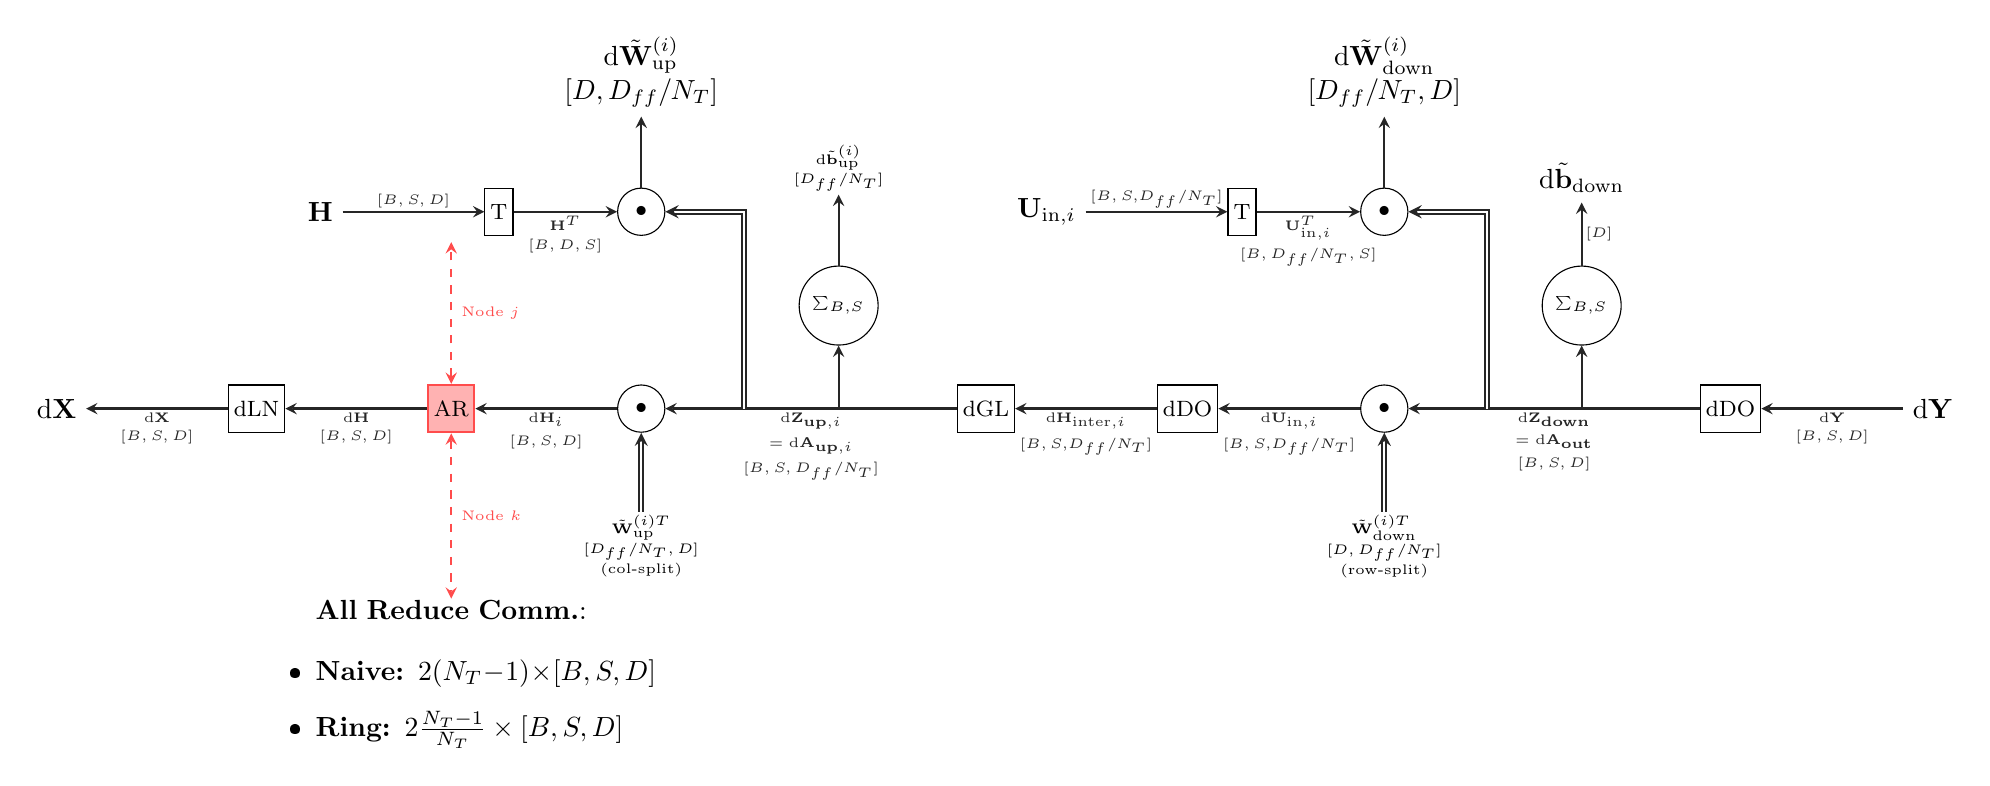
\begin{tikzpicture}[
    >=stealth,
    auxnode/.style={draw, rectangle, fill=white, minimum height=6mm, inner sep=2pt, font=\footnotesize, align=center},
    mulnode/.style={draw, circle, fill=white, minimum size=6mm, font=\footnotesize, align=center},
    addnode/.style={draw, circle, fill=white, minimum size=6mm, font=\footnotesize, align=center},
    sumnode/.style={draw, circle, fill=white, minimum size=6mm, font=\tiny, align=center},
    allreduce/.style={draw, rectangle, fill=red!30, minimum height=6mm, inner sep=2pt, font=\footnotesize, align=center, thick, draw=red!70},
    flow_rev/.style={<-, thick, black!85},
    flow_dw/.style={->, thick, black!85},
    flow_act/.style={double, ->, thick, black!85},
    commflow/.style={<->, thick, red!70, dashed},
    dimlabel/.style={font=\tiny, inner sep=1pt, align=center},
    gradlabel/.style={font=\tiny\bfseries, inner sep=1pt, align=center}
]
    % \node[font=\Large\bfseries] at (5, 10) {MLP Backward Pass (Node $i$)};

    \pgfmathsetmacro{\backwardoffset}{0.0}

    \node (d_MOut) at (12.6, \backwardoffset) {$\mathrm{d}\mathbf{Y}$};
    \node[auxnode] (d_Drop2) [left=1.8cm of d_MOut] {dDO};
    \draw[flow_rev] (d_Drop2) -- (d_MOut)
      node[dimlabel, midway, below]{\shortstack{$\mathrm{d}\mathbf{Y}$\\$[B,S,D]$}};

    \coordinate (split2) at ($(d_Drop2.west) + (-1.5cm, 0)$);
    \coordinate (branch_dUproj) at ($(split2) + (-1.2cm, 0)$);

    \node[sumnode] (d_SumB2) [above=0.8cm of split2] {$\sum_{B, S}$};
    \node (d_Bdown) [above=0.8cm of d_SumB2] {$\mathrm{d}\tilde{\mathbf{b}}_{\text{down}}$};
    \draw[flow_dw] (d_SumB2) -- (d_Bdown) node[dimlabel, midway, right]{$[D]$};

    \draw[flow_rev] (d_SumB2) -- (split2);

    \node[mulnode] (d_L2Mul_in) [left=2.2cm of split2] {$\bullet$};
    \draw[flow_rev] (d_L2Mul_in) -- (d_Drop2)
      node[gradlabel, midway, below]{\shortstack{$\mathrm{d}\mathbf{Z}_{\text{down}}$\\$=\mathrm{d}\mathbf{A}_{\text{out}}$\\$[B,S,D]$}};

    \node[dimlabel] (W_down_T) [align=center, below=1.0cm of d_L2Mul_in] {$\tilde{\mathbf{W}}_{\text{down}}^{(i)T}$\\$[D, D_{ff}/N_T]$\\(row-split)};
    \draw[flow_act] (W_down_T.north) -- (d_L2Mul_in);

    \coordinate (L2Mul_w_y) at ($(d_L2Mul_in) + (0, 2.5cm)$);
    \node[mulnode] (d_L2Mul_w) at (L2Mul_w_y) {$\bullet$};
    \node (d_Wdown) [align=center, above=0.9cm of d_L2Mul_w] {$\mathrm{d}\tilde{\mathbf{W}}_{\text{down}}^{(i)}$\\$[D_{ff}/N_T, D]$};
    \draw[flow_dw] (d_L2Mul_w) -- (d_Wdown);

    \draw[flow_act] (branch_dUproj.north) |- (d_L2Mul_w.east);

    \node[auxnode] (Uin_T) at ($(d_L2Mul_w.west) + (-1.5cm, 0)$) {T};
    \draw[flow_dw] (Uin_T) -- (d_L2Mul_w)
      node[dimlabel, midway, below]{\shortstack{$\mathbf{U}_{\text{in},i}^T$\\$[B, D_{ff}/N_T, S]$}};
    \node (Uin_aux) [left=1.8cm of Uin_T] {$\mathbf{U}_{\text{in},i}$};
    \draw[flow_dw] (Uin_aux) -- (Uin_T) node[dimlabel, midway, above]{\shortstack{$[B,S,$$D_{ff}/N_T]$}};

    \node[auxnode] (d_Drop1) [left=1.8cm of d_L2Mul_in] {dDO};
    \draw[flow_rev] (d_Drop1) -- (d_L2Mul_in)
      node[dimlabel, midway, below]{\shortstack{$\mathrm{d}\mathbf{U}_{\text{in},i}$\\$[B,S,$$D_{ff}/N_T]$}};

    \node[auxnode] (d_Act) [left=1.8cm of d_Drop1] {dGL};
    \draw[flow_rev] (d_Act) -- (d_Drop1)
      node[dimlabel, midway, below]{\shortstack{$\mathrm{d}\mathbf{H}_{\text{inter},i}$\\$[B,S,$$D_{ff}/N_T]$}};

    \coordinate (split1) at ($(d_Act.west) + (-1.5cm, 0)$);
    \coordinate (branch_dHpre) at ($(split1) + (-1.2cm, 0)$);

    \node[sumnode] (d_SumB1) [above=0.8cm of split1] {$\sum_{B, S}$};
    \node[dimlabel] (d_Bup) [above=0.9cm of d_SumB1] {$\mathrm{d}\tilde{\mathbf{b}}_{\text{up}}^{(i)}$\\$[D_{ff}/N_T]$};
    \draw[flow_dw] (d_SumB1) -- (d_Bup);

    \draw[flow_rev] (d_SumB1) -- (split1);

    \node[mulnode] (d_L1Mul_in) [left=2.2cm of split1] {$\bullet$};
    \draw[flow_rev] (d_L1Mul_in) -- (d_Act)
      node[gradlabel, midway, below]{\shortstack{$\mathrm{d}\mathbf{Z}_{\text{up},i}$\\$=\mathrm{d}\mathbf{A}_{\text{up},i}$\\$[B,S,D_{ff}/N_T]$}};

    \node[dimlabel] (W_up_T) [align=center, below=1.0cm of d_L1Mul_in] {$\tilde{\mathbf{W}}_{\text{up}}^{(i)T}$\\$[D_{ff}/N_T, D]$\\(col-split)};
    \draw[flow_act] (W_up_T.north) -- (d_L1Mul_in);

    \coordinate (L1Mul_w_y) at ($(d_L1Mul_in) + (0, 2.5cm)$);
    \node[mulnode] (d_L1Mul_w) at (L1Mul_w_y) {$\bullet$};
    \node (d_Wup) [align=center, above=0.9cm of d_L1Mul_w] {$\mathrm{d}\tilde{\mathbf{W}}_{\text{up}}^{(i)}$\\$[D, D_{ff}/N_T]$};
    \draw[flow_dw] (d_L1Mul_w) -- (d_Wup);

    \draw[flow_act] (branch_dHpre.north) |- (d_L1Mul_w.east);

    \node[auxnode] (Znorm_T) at ($(d_L1Mul_w.west) + (-1.5cm, 0)$) {T};
    \draw[flow_dw] (Znorm_T) -- (d_L1Mul_w)
      node[dimlabel, midway, below]{\shortstack{$\mathbf{H}^T$\\$[B, D, S]$}};
    \node (Znorm_aux) [left=1.8cm of Znorm_T] {$\mathbf{H}$};
    \draw[flow_dw] (Znorm_aux) -- (Znorm_T) node[dimlabel, midway, above]{\shortstack{$[B,S,D]$}};

    \node[allreduce] (AR) [left=1.8cm of d_L1Mul_in] {AR};
    \node[
      align=center,
      below=2.0cm of AR,
      text width=5.2cm
    ] (AR_info) {%
      \textbf{All Reduce Comm.}:\\[2pt]
      \begin{itemize}
        \item \textbf{Naive:} $2(N_T-1) \times [B,S,D]$
        \item \textbf{Ring:} $2\frac{N_T-1}{N_T} \times [B,S,D]$
      \end{itemize}
    };

    % All-Reduce communication arrows
    \draw[commflow] (AR.north) -- ++(0, 1.8) node[midway, right, font=\tiny]{Node $j$};
    \draw[commflow] (AR.south) -- ++(0, -2.1) node[midway, right, font=\tiny]{Node $k$};

    \draw[flow_rev] (AR) -- (d_L1Mul_in)
      node[dimlabel, midway, below]{\shortstack{$\mathrm{d}\mathbf{H}_i$\\$[B,S,D]$}};

    \node[auxnode] (d_LN2) [left=1.8cm of AR] {dLN};
    \draw[flow_rev] (d_LN2) -- (AR)
      node[dimlabel, midway, below]{\shortstack{$\mathrm{d}\mathbf{H}$\\$[B,S,D]$}};

    \node (d_MIn) [left=1.8cm of d_LN2] {$\mathrm{d}\mathbf{X}$};
    \draw[flow_rev] (d_MIn) -- (d_LN2)
      node[dimlabel, midway, below]{\shortstack{$\mathrm{d}\mathbf{X}$\\$[B,S,D]$}};
\end{tikzpicture}%
}

\clearpage

% ==========================================================
% 6. Data Parallelism (DP)
% ==========================================================
\section{Data Parallelism (DP)}

In data parallelism, each replica holds a full copy of the model, but
processes a different subset of the batch. Gradients are synchronized
across replicas via All-Reduce.

\subsection{DP Overview and Transformer Flow}
\resizebox{\linewidth}{!}{%
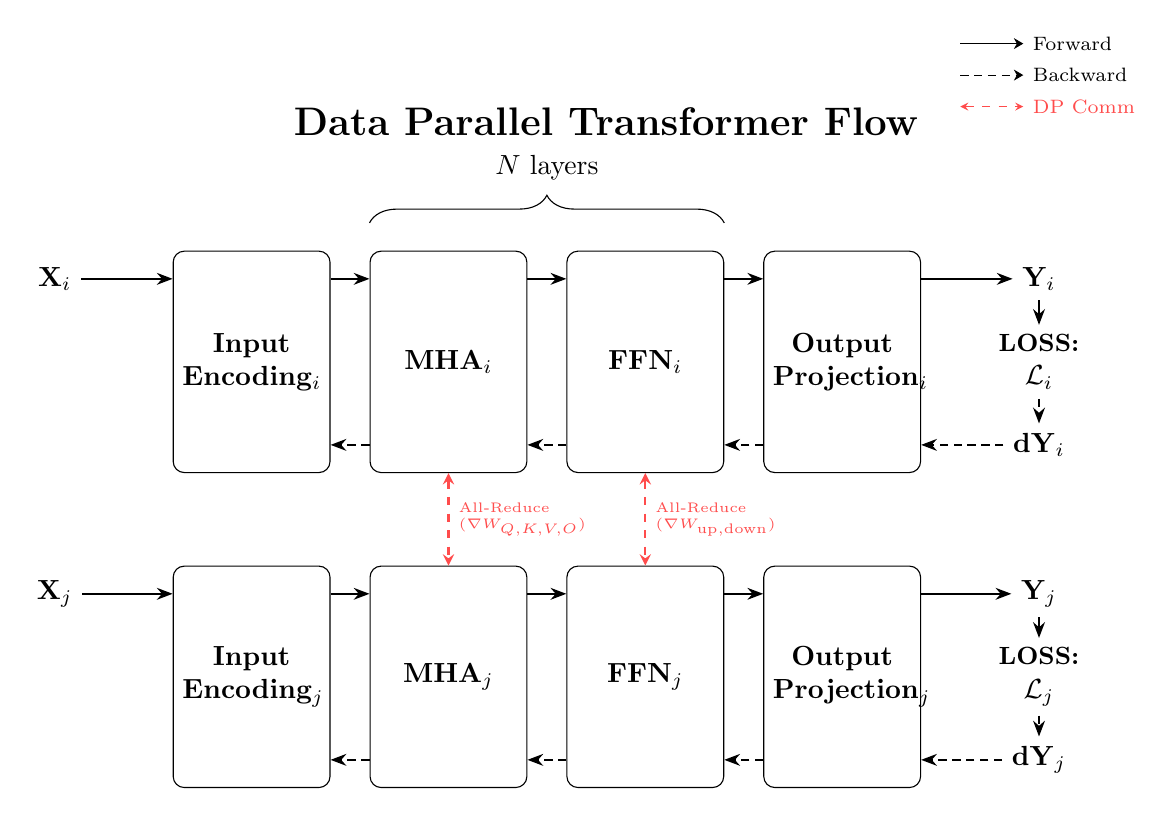
\begin{tikzpicture}[
    node distance=2.5cm,
    >=stealth,
    block/.style={rectangle, draw=black, fill=white, text width=5em, text centered, rounded corners, minimum height=8em, font=\bfseries},
    forward/.style={-{Stealth[length=2mm]}, thick, black},
    backward/.style={-{Stealth[length=2mm]}, thick, black, densely dashed},
    dpcomm/.style={<->, thick, red!70, dashed},
    io/.style={text centered, font=\bfseries}
]
    % Title
    \node[font=\Large\bfseries] at (7, 12) {Data Parallel Transformer Flow};

    % ========== Node i (Upper) ==========
    \node (input_i) [io] at (0, 10) {$\mathbf{X}_i$};
    \node (encoding_i) [block, right of=input_i, yshift=-3em] {Input\\Encoding$_i$};
    \node (mha_i) [block, right of=encoding_i] {MHA$_i$};
    \node (mlp_i) [block, right of=mha_i] {FFN$_i$};
    \node (output_i) [block, right of=mlp_i] {Output\\Projection$_i$};
    \node (pred_i) [io, right of=output_i, yshift=3em] {$\mathbf{Y}_i$};
    \node (loss_i) [align=center, io, right of=output_i] {\small LOSS:\\$\mathcal{L}_i$};
    \node (gradient_i) [io, right of=output_i, yshift=-3em] {$\mathbf{dY}_i$};

    % Forward arrows - Node i
    \draw [forward] (input_i) -- ([yshift=3em]encoding_i.west);
    \draw [forward] ([yshift=3em]encoding_i.east) -- ([yshift=3em]mha_i.west);
    \draw [forward] ([yshift=3em]mha_i.east) -- ([yshift=3em]mlp_i.west);
    \draw [forward] ([yshift=3em]mlp_i.east) -- ([yshift=3em]output_i.west);
    \draw [forward] ([yshift=3em]output_i.east) -- (pred_i);
    \draw [forward] (pred_i) -- (loss_i);
    \draw [backward] (loss_i) -- (gradient_i);

    % Backward arrows - Node i
    \draw [backward] (gradient_i) -- ([yshift=-3em]output_i.east);
    \draw [backward] ([yshift=-3em]output_i.west) -- ([yshift=-3em]mlp_i.east);
    \draw [backward] ([yshift=-3em]mlp_i.west) -- ([yshift=-3em]mha_i.east);
    \draw [backward] ([yshift=-3em]mha_i.west) -- ([yshift=-3em]encoding_i.east);

    % Brace for layer repetition - Node i
    \draw[decorate, decoration={brace, amplitude=10pt}]
        ([yshift=1.0em]mha_i.north west) -- ([yshift=1.0em]mlp_i.north east)
        node[midway, above=12pt, font=\normalsize] {$N$ layers};

    % ========== Node j (Lower) ==========
    \node (input_j) [io] at (0, 6) {$\mathbf{X}_j$};
    \node (encoding_j) [block, right of=input_j, yshift=-3em] {Input\\Encoding$_j$};
    \node (mha_j) [block, right of=encoding_j] {MHA$_j$};
    \node (mlp_j) [block, right of=mha_j] {FFN$_j$};
    \node (output_j) [block, right of=mlp_j] {Output\\Projection$_j$};
    \node (pred_j) [io, right of=output_j, yshift=3em] {$\mathbf{Y}_j$};
    \node (loss_j) [align=center, io, right of=output_j] {\small LOSS:\\$\mathcal{L}_j$};
    \node (gradient_j) [io, right of=output_j, yshift=-3em] {$\mathbf{dY}_j$};

    % Forward arrows - Node j
    \draw [forward] (input_j) -- ([yshift=3em]encoding_j.west);
    \draw [forward] ([yshift=3em]encoding_j.east) -- ([yshift=3em]mha_j.west);
    \draw [forward] ([yshift=3em]mha_j.east) -- ([yshift=3em]mlp_j.west);
    \draw [forward] ([yshift=3em]mlp_j.east) -- ([yshift=3em]output_j.west);
    \draw [forward] ([yshift=3em]output_j.east) -- (pred_j);
    \draw [forward] (pred_j) -- (loss_j);
    \draw [backward] (loss_j) -- (gradient_j);

    % Backward arrows - Node j
    \draw [backward] (gradient_j) -- ([yshift=-3em]output_j.east);
    \draw [backward] ([yshift=-3em]output_j.west) -- ([yshift=-3em]mlp_j.east);
    \draw [backward] ([yshift=-3em]mlp_j.west) -- ([yshift=-3em]mha_j.east);
    \draw [backward] ([yshift=-3em]mha_j.west) -- ([yshift=-3em]encoding_j.east);

    % ========== DP Communications ==========
    \draw [dpcomm] (mha_i.south) -- (mha_j.north) node[midway, right, font=\tiny, align=left] {All-Reduce\\$(\nabla W_{Q,K,V,O})$};
    \draw [dpcomm] (mlp_i.south) -- (mlp_j.north) node[midway, right, font=\tiny, align=left] {All-Reduce\\$(\nabla W_{\text{up},\text{down}})$};

    % Labels (Legend)
    \coordinate (legend) at ([xshift=11.5cm, yshift=8.5em]input_i);

    % Forward (작은 화살표 + 작은 글자)
    \draw[
        forward,
        -{Stealth[length=1.2mm,width=1.4mm]}, % 화살표 더 작게
        line width=0.3pt                       % 선 더 얇게
    ] (legend) -- ++(0.8,0)
      node[right, font=\scriptsize] {Forward};

    % Backward
    \draw[
        backward,
        -{Stealth[length=1.2mm,width=1.4mm]},
        line width=0.3pt
    ] ([yshift=-0.4cm]legend) -- ++(0.8,0)
      node[right, font=\scriptsize] {Backward};

    % DP Comm
    \draw[
        dpcomm,
        line width=0.3pt
    ] ([yshift=-0.8cm]legend) -- ++(0.8,0)
      node[right, font=\scriptsize] {DP Comm};
\end{tikzpicture}%
}

\clearpage

\subsection{MHA Backward under DP}
\resizebox{\linewidth}{!}{%
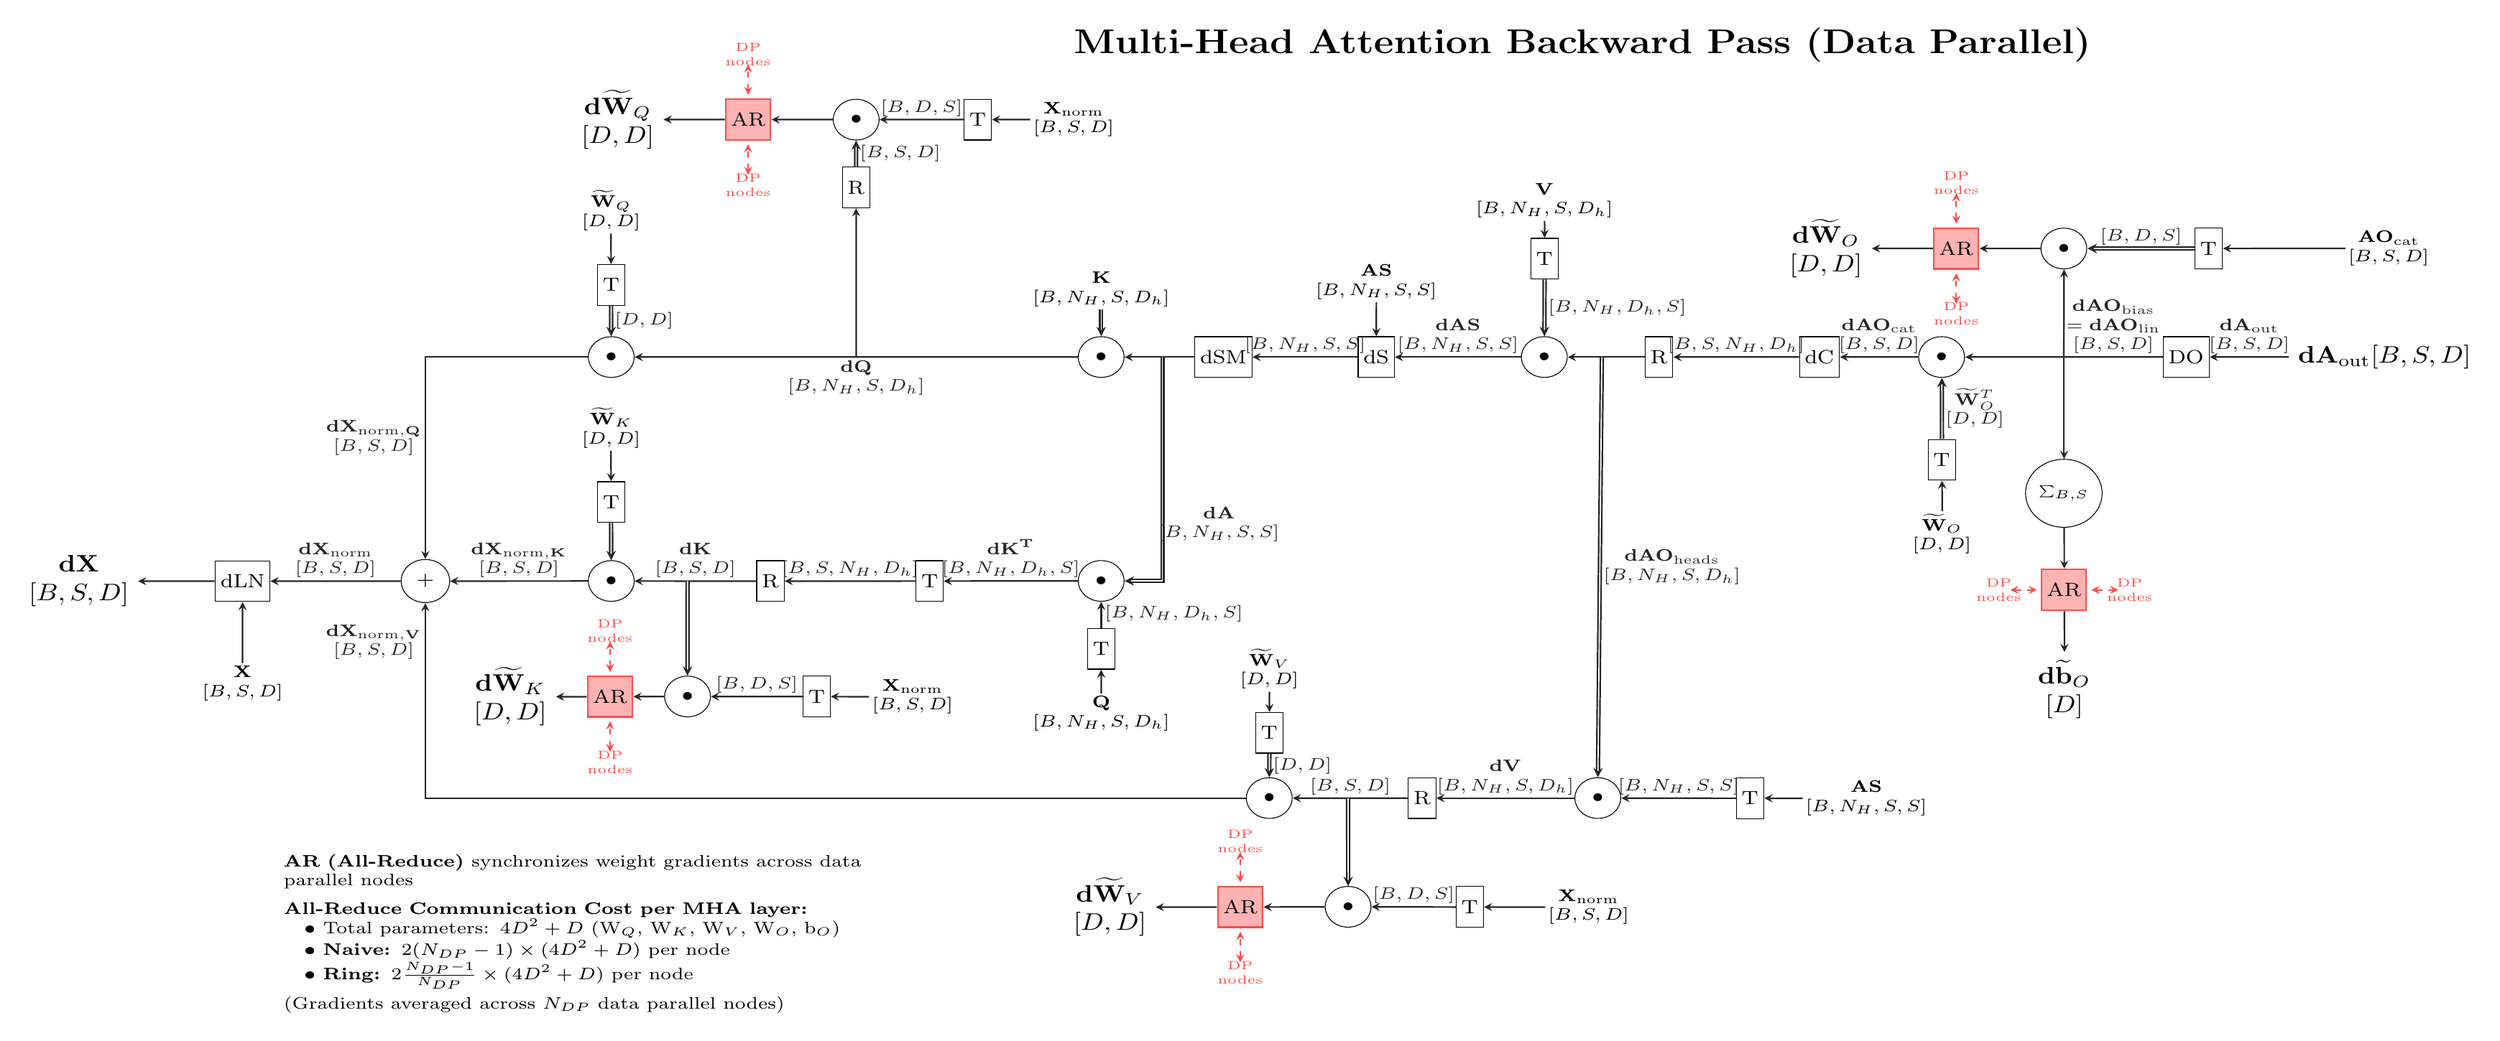
\begin{tikzpicture}[
  every node/.style={transform shape},
  >=stealth,
  auxnode/.style={draw, rectangle, fill=white, minimum height=6mm, inner sep=2pt, font=\footnotesize, align=center},
  mulnode/.style={draw, circle, fill=white, minimum size=6mm, font=\footnotesize, align=center},
  addnode/.style={draw, circle, fill=white, minimum size=6mm, font=\footnotesize, align=center},
  sumnode/.style={draw, circle, fill=white, minimum size=6mm, font=\tiny, align=center},
  arnode/.style={draw, rectangle, fill=red!30, minimum height=6mm, inner sep=2pt, font=\footnotesize, align=center, thick, draw=red!70},
  flow/.style={->, thick, black!85},
  flow2/.style={->, double, thick, black!85},
  dimlabel/.style={font=\scriptsize, inner sep=1pt, align=center},
  gradflow/.style={->, thick, black!85},
  gradweight/.style={->, thick, black!85},
  dpgradweight/.style={->, thick, black!85},
  dpcomm/.style={<->, thick, red!70, dashed}
]

\begin{scope}[xscale=1.35, yscale=1.2]

\def\yoffset{-1.0}
\def\dVXyoffset{-6.5}

\coordinate (Grad_Aout_B) at (17.5, \yoffset);
\coordinate (dDrop_center) at (15.9, \yoffset);
\coordinate (ProjGradSplit) at (14.3, \yoffset);
\coordinate (dOProj_center) at (12.7, \yoffset);
\coordinate (C_center) at (11.1, \yoffset);
\coordinate (R_center) at (9.0, \yoffset);
\coordinate (dPV_AS_calc_center) at (7.5, \yoffset);
\coordinate (dSoft_center) at (5.3, \yoffset);
\coordinate (dSM_calc_center) at (3.3, \yoffset);
\coordinate (dV_calc_center) at (8.2, \dVXyoffset+\yoffset);
\coordinate (R_V_bwd_center) at (5.9, \dVXyoffset+\yoffset);
\coordinate (dVX_calc_center) at (3.9, \dVXyoffset+\yoffset);
\coordinate (dQK_calc_Q_center) at (1.7, \yoffset);
\coordinate (dQK_calc_K_center) at (1.7, -3.3+\yoffset);
\coordinate (K_BWD_input_center) at (1.7, 1.0+\yoffset);
\coordinate (T_Q_bwd_center) at (1.7, -4.3+\yoffset);

\node[font=\Large\bfseries] at (8, 4.6+\yoffset) {Multi-Head Attention Backward Pass (Data Parallel)};

\node (Grad_Aout_B) at (18.5, \yoffset) {$\mathbf{dA}_{\text{out}}$\\$[B,S,D]$};
\node[auxnode] (DO) at (dDrop_center) {DO};
\node[mulnode] (dOProj) at (dOProj_center) {$\bullet$};

\node[auxnode] (T_WO) [below=0.9cm of dOProj] {T};
\node[dimlabel] (WO_BWD) [below=0.45cm of T_WO] {$\widetilde{\mathbf{W}}_{O}$\\$[D,D]$};

\node[mulnode] (dWO_calc) at ($(ProjGradSplit)+(0, 1.6)$) {$\bullet$};

% Add AR node before dWO
\node[arnode] (AR_WO) [left=0.8cm of dWO_calc] {AR};
\draw[dpcomm] ([yshift=-0.5cm]AR_WO.south) -- ([yshift=-0.05cm]AR_WO.south);
\draw[dpcomm] ([yshift=0.05cm]AR_WO.north) -- ([yshift=0.5cm]AR_WO.north);
\node[font=\tiny, red!70, align=center] at ([yshift=-0.65cm]AR_WO.south) {DP\\nodes};
\node[font=\tiny, red!70, align=center] at ([yshift=0.65cm]AR_WO.north) {DP\\nodes};

\node[align=center, left=0.8cm of AR_WO]
  (dWO_GRAD) {$\mathbf{d}\widetilde{\mathbf{W}}_{O}$\\$[D,D]$};
\draw[dpgradweight] (dWO_calc) -- (AR_WO);
\draw[gradflow] (AR_WO) -- (dWO_GRAD);

\node[auxnode] (T_AO_in) [right=1.4cm of dWO_calc] {T};
\node[dimlabel] (AO_in_local_label) [right=1.6cm of T_AO_in] {$\mathbf{AO}_{\text{cat}}$\\$[B,S,D]$};

\node[auxnode] (C) at (C_center) {dC};
\node[auxnode] (R) at (R_center) {R};

\node[mulnode] (dPV_AS_calc) at (dPV_AS_calc_center) {$\bullet$};
\node[auxnode] (dSoft) at (dSoft_center) {dS};
\node[auxnode] (dSM_calc) at (dSM_calc_center) {dSM};

\node[mulnode] (dQK_calc_Q) at (dQK_calc_Q_center) {$\bullet$};
\node[mulnode] (dQX_proj_calc) [left=5.8cm of dQK_calc_Q] {$\bullet$};

\node[mulnode] (dQK_calc_K) at (dQK_calc_K_center) {$\bullet$};
\node[mulnode] (dKX_proj_calc) [left=5.8cm of dQK_calc_K] {$\bullet$};

\node[dimlabel] (K_BWD_input) at (K_BWD_input_center) {$\mathbf{K}$\\$[B,N_H,S,D_h]$};
\node[auxnode] (T_Q_bwd) at (T_Q_bwd_center) {T};
\node[dimlabel] (Q_BWD_input) [below=0.35cm of T_Q_bwd] {$\mathbf{Q}$\\$[B,N_H,S,D_h]$};

\node[dimlabel] (V_FWD) [above=1.7cm of dPV_AS_calc] {$\mathbf{V}$\\$[B,N_H,S,D_h]$};
\node[auxnode] (T_V_bwd) [below=0.25cm of V_FWD] {T};

\node[mulnode] (dV_calc) at (dV_calc_center) {$\bullet$};
\node[auxnode] (T_AS_bwd) [right=1.5cm of dV_calc] {T};
\node[dimlabel] (AS_BWD_for_V) [right=0.5cm of T_AS_bwd] {$\mathbf{AS}$\\$[B,N_H,S,S]$};

\node[auxnode] (R_V_bwd) at (R_V_bwd_center) {R};
\node[mulnode] (dVX_calc) at (dVX_calc_center) {$\bullet$};

\node[auxnode] (T_WV) [above=0.35cm of dVX_calc] {T};
\node[dimlabel] (WV_BWD) [above=0.3cm of T_WV] {$\widetilde{\mathbf{W}}_{V}$\\$[D,D]$};

\node[sumnode] (Sum_dBO) [below=1.5cm of ProjGradSplit] {$\sum_{B, S}$};

% Add AR node before dBO
\node[arnode] (AR_BO) [below=0.6cm of Sum_dBO] {AR};
\draw[dpcomm] ([xshift=-0.4cm]AR_BO.west) -- ([xshift=-0.05cm]AR_BO.west);
\draw[dpcomm] ([xshift=0.05cm]AR_BO.east) -- ([xshift=0.4cm]AR_BO.east);
\node[font=\tiny, red!70, align=center] at ([xshift=-0.55cm]AR_BO.west) {DP\\nodes};
\node[font=\tiny, red!70, align=center] at ([xshift=0.55cm]AR_BO.east) {DP\\nodes};

\node[align=center] (dBO) [below=0.6cm of AR_BO] {$\mathbf{d}\widetilde{\mathbf{b}}_{O}$\\$[D]$};
\draw[dpgradweight] (Sum_dBO) -- (AR_BO);
\draw[gradflow] (AR_BO) -- (dBO);

\draw[gradflow] (Grad_Aout_B) -- (DO)
  node[dimlabel, midway, above]{$\mathbf{dA}_{\text{out}}$\\$[B,S,D]$};

\draw[gradflow] (DO) -- (dOProj)
  node[dimlabel, pos=0.25, above]{$\mathbf{dAO}_{\text{bias}}$\\$=\mathbf{dAO}_{\text{lin}}$\\$[B,S,D]$};

\draw[gradflow] (ProjGradSplit) -- (dWO_calc.south);
\draw[gradflow] (ProjGradSplit) -- ([yshift=-0.75cm]ProjGradSplit) -| (Sum_dBO.north);

\draw[gradflow] (dOProj) -- (C)
  node[dimlabel, midway, above]{$\mathbf{dAO}_{\text{cat}}$\\$[B,S,D]$};
\draw[gradflow] (C) -- (R)
  node[dimlabel, midway, above]{$[B,S,N_H,D_h]$};

\coordinate (R_split_point) at ($(dPV_AS_calc)!0.5!(R)$);
\draw[gradflow] (R.west) -- (dPV_AS_calc.east);
\draw[flow2] (R_split_point) -- (dV_calc.north)
  node[dimlabel, midway, right]{$\mathbf{dAO}_{\text{heads}}$\\$[B,N_H,S,D_h]$};

\draw[gradflow] (V_FWD.south) -- (T_V_bwd.north);
\draw[flow2] (T_V_bwd.south) -- (dPV_AS_calc.north)
  node[dimlabel, midway, right]{$[B,N_H,D_h,S]$};
\draw[gradflow] (dPV_AS_calc.west) -- (dSoft.east)
  node[dimlabel, midway, above]{$\mathbf{dAS}$\\$[B,N_H,S,S]$};

\node (AS_BWD_dS) [dimlabel, above=0.5cm of dSoft] {$\mathbf{AS}$\\$[B,N_H,S,S]$};
\draw[gradflow] (AS_BWD_dS.south) -- (dSoft.north);
\draw[gradflow] (dSoft.west) -- (dSM_calc.east)
  node[dimlabel, midway, above]{$[B,N_H,S,S]$};

\coordinate (dA_Split_X) at ($(dSM_calc_center)!0.5!(dQK_calc_Q_center)$);
\coordinate (dA_Split) at (dA_Split_X |- dQK_calc_Q.east);
\draw[gradflow] (dSM_calc.west) -- (dQK_calc_Q.east);
\draw[flow2] (dA_Split) -- (dA_Split |- dQK_calc_K.east) -- (dQK_calc_K.east)
  node[dimlabel, pos=-1.5, above, yshift=15]{$\mathbf{dA}$\\$[B,N_H,S,S]$};

\draw[flow2] (K_BWD_input.south) -- (dQK_calc_Q.north);
\draw[gradweight] (dQK_calc_Q) -- (dQX_proj_calc)
  node[dimlabel, midway, below]{$\mathbf{dQ}$\\$[B,N_H,S,D_h]$};

\node[auxnode] (T_WQ_bwd) [above=0.45cm of dQX_proj_calc] {T};
\node[dimlabel] (WQ_bwd) [above=0.45cm of T_WQ_bwd] {$\widetilde{\mathbf{W}}_{Q}$\\$[D,D]$};
\draw[flow] (WQ_bwd) -- (T_WQ_bwd);
\draw[flow2] (T_WQ_bwd.south) -- (dQX_proj_calc.north)
  node[dimlabel, midway, right]{$[D,D]$};

\draw[flow] (Q_BWD_input.north) -- (T_Q_bwd.south);
\draw[flow] (T_Q_bwd.north) -- (dQK_calc_K.south)
  node[dimlabel, pos=0.55, right]{$[B,N_H,D_h,S]$};

\node[auxnode] (T_dK) at ($(dQK_calc_K)!0.35!(dKX_proj_calc)$) {T};
\node[auxnode] (R_dK_mid) at ($(T_dK)!0.5!(dKX_proj_calc)$) {R};

\draw[gradweight] (dQK_calc_K) -- (T_dK)
  node[dimlabel, midway, above]{$\mathbf{dK^T}$\\$[B,N_H,D_h,S]$};
\draw[gradweight] (T_dK) -- (R_dK_mid)
  node[dimlabel, midway, above]{$[B,S,N_H,D_h]$};
\draw[gradweight] (R_dK_mid) -- (dKX_proj_calc)
  node[dimlabel, midway, above]{$\mathbf{dK}$\\$[B,S,D]$};

\node[auxnode] (T_WK_bwd) [above=0.55cm of dKX_proj_calc] {T};
\node[dimlabel] (WK_bwd) [above=0.45cm of T_WK_bwd] {$\widetilde{\mathbf{W}}_{K}$\\$[D,D]$};
\draw[gradflow] (WK_bwd) -- (T_WK_bwd);
\draw[flow2] (T_WK_bwd.south) -- (dKX_proj_calc.north);
\draw[gradflow] (AS_BWD_for_V.west) -- (T_AS_bwd.east);
\draw[gradflow] (T_AS_bwd.west) -- (dV_calc.east)
  node[dimlabel, midway, above]{$[B,N_H,S,S]$};
\draw[gradflow] (dV_calc.west) -- (R_V_bwd.east)
  node[dimlabel, midway, above]{$\mathbf{dV}$\\$[B,N_H,S,D_h]$};
\draw[gradflow] (R_V_bwd) -- (dVX_calc.east)
  node[dimlabel, midway, above]{$[B,S,D]$};

\draw[gradflow] (WV_BWD) -- (T_WV);
\draw[flow2] (T_WV) -- (dVX_calc.north)
  node[dimlabel, midway, right]{$[D,D]$};

\node[addnode] (Sum_dXnorm) [left=1.8cm of dKX_proj_calc] {$+$};

\draw[gradweight] (dQX_proj_calc.west) -| node[dimlabel, pos=0.7, left]{$\mathbf{dX}_{\text{norm},\mathbf{Q}}$\\$[B,S,D]$} (Sum_dXnorm.north);
\draw[gradweight] (dKX_proj_calc.west) -- node[dimlabel, midway, above]{$\mathbf{dX}_{\text{norm},\mathbf{K}}$\\$[B,S,D]$} (Sum_dXnorm.east);
\draw[gradweight] (dVX_calc.west) -| node[dimlabel, pos=0.9, left]{$\mathbf{dX}_{\text{norm},\mathbf{V}}$\\$[B,S,D]$} (Sum_dXnorm.south);

\coordinate (dV_branch) at ($(R_V_bwd.west)!0.52!(dVX_calc.east)$);
\node[mulnode] (dWV_mul) at ($(dV_branch)+(0,-1.6cm)$) {$\bullet$};
\draw[flow2] (dV_branch) -- (dWV_mul.north);

\node[auxnode] (T_Xnorm) [right=1.1cm of dWV_mul] {T};
\node[dimlabel] (Xnorm_local) [right=0.8cm of T_Xnorm] {$\mathbf{X}_{\text{norm}}$\\$[B,S,D]$};
\draw[gradflow] (Xnorm_local) -- (T_Xnorm);
\draw[gradflow] (T_Xnorm.west) -- (dWV_mul.east)
  node[dimlabel, midway, above]{$[B,D,S]$};

% Add AR node before dWV
\node[arnode] (AR_WV) [left=0.8cm of dWV_mul] {AR};
\draw[dpcomm] ([yshift=-0.5cm]AR_WV.south) -- ([yshift=-0.05cm]AR_WV.south);
\draw[dpcomm] ([yshift=0.05cm]AR_WV.north) -- ([yshift=0.5cm]AR_WV.north);
\node[font=\tiny, red!70, align=center] at ([yshift=-0.65cm]AR_WV.south) {DP\\nodes};
\node[font=\tiny, red!70, align=center] at ([yshift=0.65cm]AR_WV.north) {DP\\nodes};

\node[align=center] (dWV_out) [left=0.8cm of AR_WV] {$\mathbf{d}\widetilde{\mathbf{W}}_{V}$\\$[D,D]$};
\draw[dpgradweight] (dWV_mul.west) -- (AR_WV);
\draw[gradflow] (AR_WV) -- (dWV_out);

\coordinate (dQ_branch) at ($(dQK_calc_Q.east)!0.50!(dQX_proj_calc.west)$);
\node[mulnode] (dWQ_mul) at ($(dQ_branch)+(0,3.5cm)$) {$\bullet$};
\node[auxnode] (R_dQ_for_WQ) at ($(dWQ_mul)+(0,-1.0cm)$) {R};
\draw[gradflow]  (dQ_branch) -- (R_dQ_for_WQ.south);
\draw[flow2] (R_dQ_for_WQ.north) -- (dWQ_mul.south)
  node[dimlabel, midway, right]{$[B,S,D]$};

\node[auxnode] (T_XnormQ) [right=1.1cm of dWQ_mul] {T};
\node[dimlabel] (Xnorm_localQ) [right=0.5cm of T_XnormQ] {$\mathbf{X}_{\text{norm}}$\\$[B,S,D]$};
\draw[gradflow] (Xnorm_localQ) -- (T_XnormQ);
\draw[gradflow] (T_XnormQ.west) -- (dWQ_mul.east)
  node[dimlabel, midway, above]{$[B,D,S]$};

% Add AR node before dWQ
\node[arnode] (AR_WQ) [left=0.8cm of dWQ_mul] {AR};
\draw[dpcomm] ([yshift=-0.5cm]AR_WQ.south) -- ([yshift=-0.05cm]AR_WQ.south);
\draw[dpcomm] ([yshift=0.05cm]AR_WQ.north) -- ([yshift=0.5cm]AR_WQ.north);
\node[font=\tiny, red!70, align=center] at ([yshift=-0.65cm]AR_WQ.south) {DP\\nodes};
\node[font=\tiny, red!70, align=center] at ([yshift=0.65cm]AR_WQ.north) {DP\\nodes};

\node[align=center] (dWQ_out) [left=0.8cm of AR_WQ] {$\mathbf{d}\widetilde{\mathbf{W}}_{Q}$\\$[D,D]$};
\draw[dpgradweight] (dWQ_mul.west) -- (AR_WQ);
\draw[gradflow] (AR_WQ) -- (dWQ_out);

\coordinate (dK_branch) at ($(R_dK_mid)!0.52!(dKX_proj_calc)$);
\node[mulnode] (dWK_mul) at ($(dK_branch)+(0,-1.7cm)$) {$\bullet$};
\draw[flow2]  (dK_branch) -- (dWK_mul.north);

\node[auxnode] (T_XnormK) [right=1.2cm of dWK_mul] {T};
\node[dimlabel, right=0.5cm of T_XnormK] (Xnorm_localK) {$\mathbf{X}_{\text{norm}}$\\$[B,S,D]$};
\draw[gradflow] (Xnorm_localK) -- (T_XnormK);
\draw[gradflow] (T_XnormK.west) -- (dWK_mul.east)
  node[dimlabel, midway, above]{$[B,D,S]$};

% Add AR node before dWK
\node[arnode] (AR_WK) [left=0.4cm of dWK_mul] {AR};
\draw[dpcomm] ([yshift=-0.5cm]AR_WK.south) -- ([yshift=-0.05cm]AR_WK.south);
\draw[dpcomm] ([yshift=0.05cm]AR_WK.north) -- ([yshift=0.5cm]AR_WK.north);
\node[font=\tiny, red!70, align=center] at ([yshift=-0.65cm]AR_WK.south) {DP\\nodes};
\node[font=\tiny, red!70, align=center] at ([yshift=0.65cm]AR_WK.north) {DP\\nodes};

\node[align=center] (dWK_out) [left=0.4cm of AR_WK] {$\mathbf{d}\widetilde{\mathbf{W}}_{K}$\\$[D,D]$};
\draw[dpgradweight] (dWK_mul.west) -- (AR_WK);
\draw[gradflow] (AR_WK) -- (dWK_out);

\draw[gradflow] (WO_BWD) -- (T_WO);
\draw[flow2] (T_WO) -- (dOProj)
  node[dimlabel, midway, right]{$\widetilde{\mathbf{W}}_{O}^{T}$\\$[D,D]$};
\draw[gradflow] (AO_in_local_label) -- (T_AO_in);
\draw[flow2] (T_AO_in) -- (dWO_calc.east)
  node[dimlabel, midway, above]{$[B,D,S]$};

\node[auxnode] (dLN) [left=1.7cm of Sum_dXnorm] {dLN};
\draw[gradweight] (Sum_dXnorm.west) -- node[dimlabel, midway, above]
  {$\mathbf{dX}_{\text{norm}}$\\$[B,S,D]$} (dLN.east);

\node (dX_OUT) [align=center, left=1.0cm of dLN] {$\mathbf{dX}$\\$[B,S,D]$};
\draw[gradweight] (dLN.west) -- (dX_OUT);

\node[dimlabel] (LNCache) [below=0.9cm of dLN] {$\mathbf{X}$\\$[B,S,D]$};
\draw[gradflow] (LNCache.north) -- (dLN.south);

% Legend and explanation
    \node[align=left, font=\scriptsize, text width=8cm] at (-5, -9.5) {
      \textbf{AR (All-Reduce)} synchronizes weight gradients across data parallel nodes\\[4pt]
      \textbf{All-Reduce Communication Cost per MHA layer:}\\
      \quad • Total parameters: $4D^2 + D$ (W$_Q$, W$_K$, W$_V$, W$_O$, b$_O$)\\
      \quad • \textbf{Naive:} $2(N_{DP}-1) \times (4D^2 + D)$ per node\\
      \quad • \textbf{Ring:} $2\frac{N_{DP}-1}{N_{DP}} \times (4D^2 + D)$ per node\\[2pt]
      {\scriptsize (Gradients averaged across $N_{DP}$ data parallel nodes)}
    };

\end{scope}
\end{tikzpicture}
}

\clearpage

\subsection{MLP Backward under DP}
\noindent
\resizebox{\linewidth}{!}{%
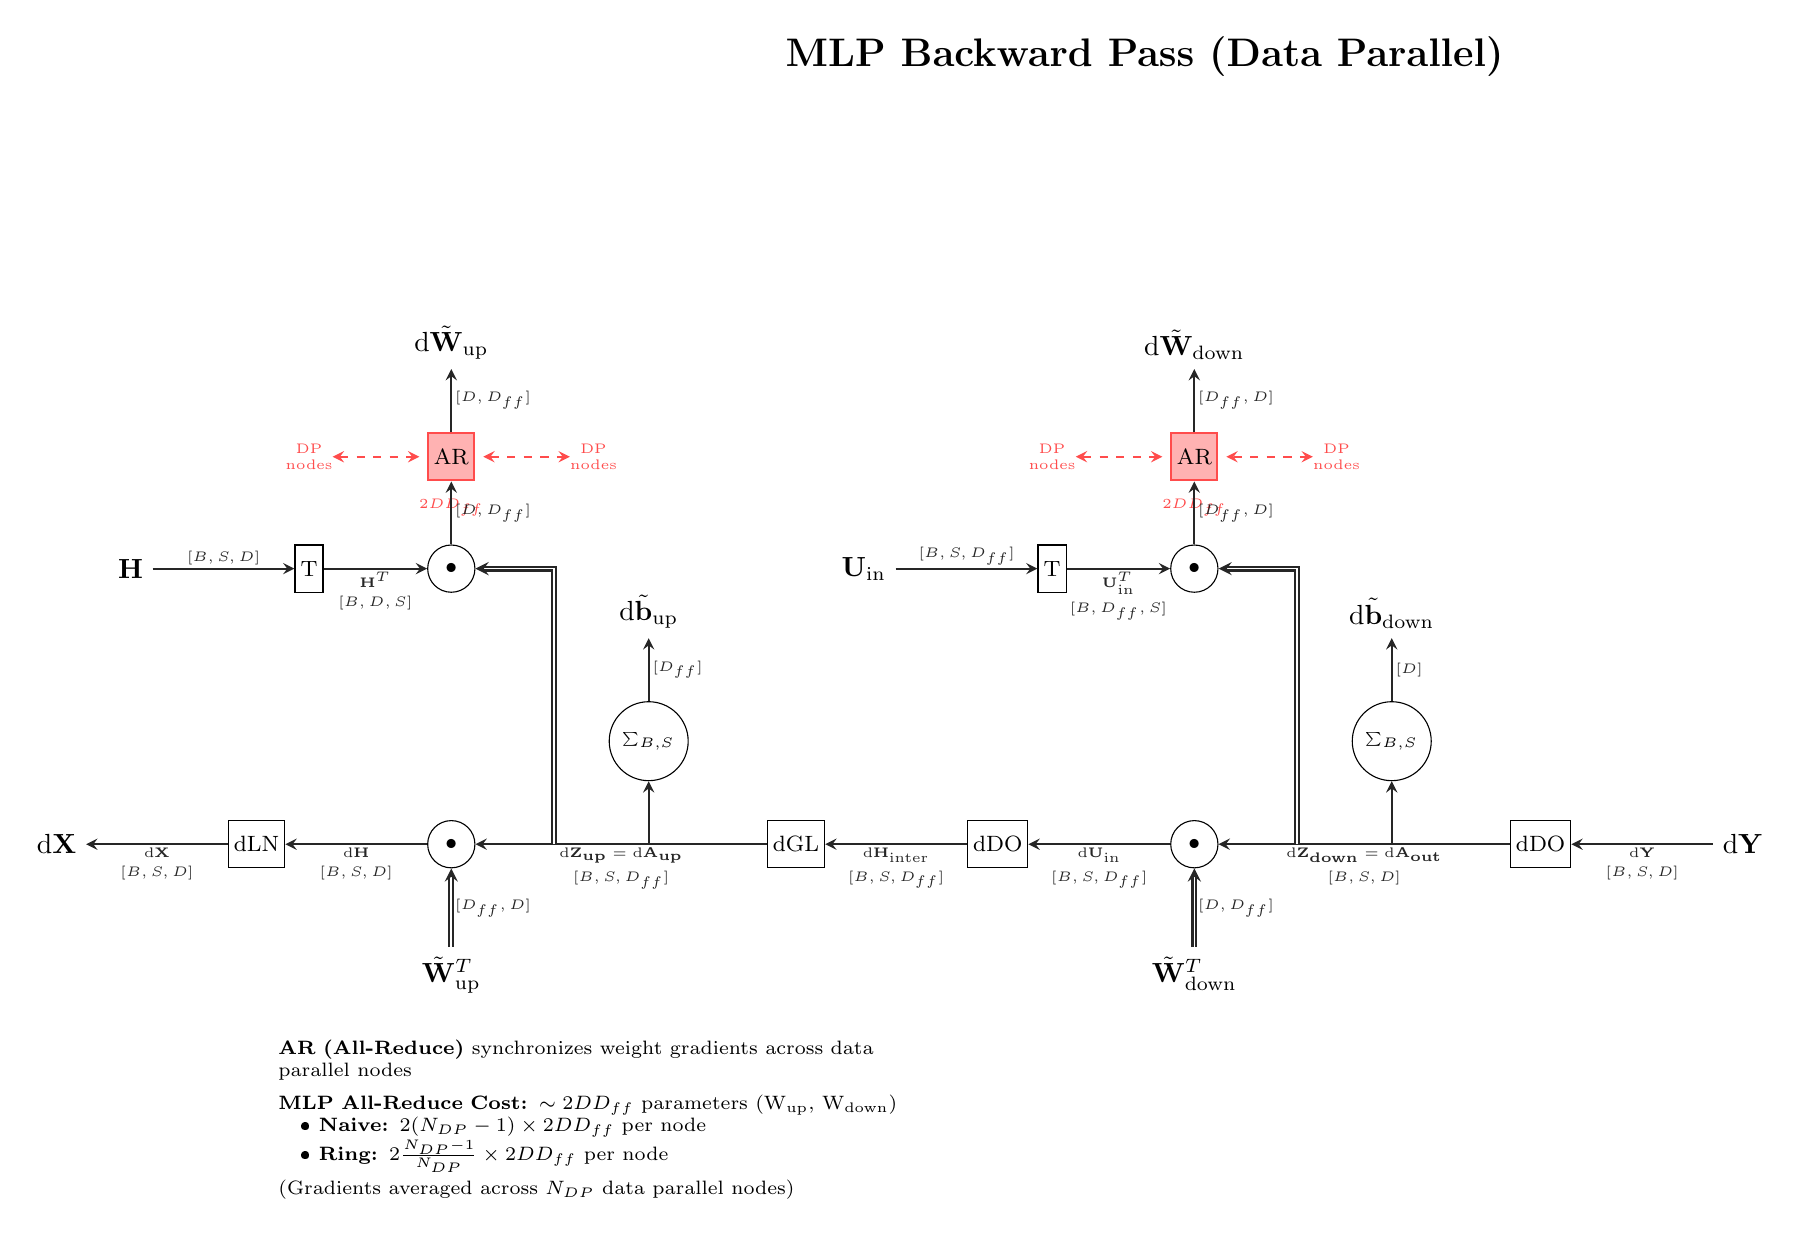
\begin{tikzpicture}[
    >=stealth,
    auxnode/.style={draw, rectangle, fill=white, minimum height=6mm, inner sep=2pt, font=\footnotesize, align=center},
    mulnode/.style={draw, circle, fill=white, minimum size=6mm, font=\footnotesize, align=center},
    addnode/.style={draw, circle, fill=white, minimum size=6mm, font=\footnotesize, align=center},
    sumnode/.style={draw, circle, fill=white, minimum size=6mm, font=\tiny, align=center},
    arnode/.style={draw, rectangle, fill=red!30, minimum height=6mm, inner sep=2pt, font=\footnotesize, align=center, thick, draw=red!70},
    flow_rev/.style={<-, thick, black!85},
    flow_dw/.style={->, thick, black!85},
    flow_act/.style={double, ->, thick, black!85},
    dimlabel/.style={font=\tiny, inner sep=1pt, align=center},
    gradlabel/.style={font=\tiny\bfseries, inner sep=1pt, align=center},
    dpgradweight/.style={->, thick, black!85},
    dpcomm/.style={<->, thick, red!70, dashed}
]
    \node[font=\Large\bfseries] at (5, 10) {MLP Backward Pass (Data Parallel)};

    \pgfmathsetmacro{\backwardoffset}{0.0}

    \node (d_MOut) at (12.6, \backwardoffset) {$\mathrm{d}\mathbf{Y}$};
    \node[auxnode] (d_Drop2) [left=1.8cm of d_MOut] {dDO};
    \draw[flow_rev] (d_Drop2) -- (d_MOut)
      node[dimlabel, midway, below]{\shortstack{$\mathrm{d}\mathbf{Y}$\\$[B,S,D]$}};

    \coordinate (split2) at ($(d_Drop2.west) + (-1.5cm, 0)$);
    \coordinate (branch_dUproj) at ($(split2) + (-1.2cm, 0)$);

    \node[sumnode] (d_SumB2) [above=0.8cm of split2] {$\sum_{B, S}$};
    \node (d_Bdown) [above=0.8cm of d_SumB2] {$\mathrm{d}\tilde{\mathbf{b}}_{\text{down}}$};
    \draw[dpgradweight] (d_SumB2) -- (d_Bdown) node[dimlabel, midway, right]{$[D]$};

    \draw[flow_rev] (d_SumB2) -- (split2);

    \node[mulnode] (d_L2Mul_in) [left=2.2cm of split2] {$\bullet$};
    \draw[flow_rev] (d_L2Mul_in) -- (d_Drop2)
      node[gradlabel, midway, below]{\shortstack{$\mathrm{d}\mathbf{Z}_{\text{down}}=\mathrm{d}\mathbf{A}_{\text{out}}$\\$[B,S,D]$}};

    \node (W_down_T) [below=1.0cm of d_L2Mul_in] {$\tilde{\mathbf{W}}_{\text{down}}^{T}$};
    \draw[flow_act] (W_down_T.north) -- (d_L2Mul_in)
      node[dimlabel, midway, right]{$[D, D_{ff}]$};

    \coordinate (L2Mul_w_y) at ($(d_L2Mul_in) + (0, 3.5cm)$);
    \node[mulnode] (d_L2Mul_w) at (L2Mul_w_y) {$\bullet$};

    % Add AR node before d_Wdown
    \node[arnode] (AR_down) [above=0.8cm of d_L2Mul_w] {AR};

    % Add communication arrows for AR_down
    \draw[dpcomm] ([xshift=-1.2cm]AR_down.west) -- ([xshift=-0.1cm]AR_down.west);
    \draw[dpcomm] ([xshift=0.1cm]AR_down.east) -- ([xshift=1.2cm]AR_down.east);
    \node[font=\tiny, red!70, align=center] at ([xshift=-1.5cm]AR_down.west) {DP\\nodes};
    \node[font=\tiny, red!70, align=center] at ([xshift=1.5cm]AR_down.east) {DP\\nodes};
    \node[font=\tiny, red!70, below=0.1cm of AR_down] {$2DD_{ff}$};

    \node (d_Wdown) [above=0.8cm of AR_down] {$\mathrm{d}\tilde{\mathbf{W}}_{\text{down}}$};
    \draw[dpgradweight] (d_L2Mul_w) -- (AR_down) node[dimlabel, midway, right]{$[D_{ff}, D]$};
    \draw[flow_dw] (AR_down) -- (d_Wdown) node[dimlabel, midway, right]{$[D_{ff}, D]$};

    \draw[flow_act] (branch_dUproj.north) |- (d_L2Mul_w.east);

    \node[auxnode] (Uin_T) at ($(d_L2Mul_w.west) + (-1.5cm, 0)$) {T};
    \draw[flow_dw] (Uin_T) -- (d_L2Mul_w)
      node[dimlabel, midway, below]{\shortstack{$\mathbf{U}_{\text{in}}^T$\\$[B, D_{ff}, S]$}};
    \node (Uin_aux) [left=1.8cm of Uin_T] {$\mathbf{U}_{\text{in}}$};
    \draw[flow_dw] (Uin_aux) -- (Uin_T) node[dimlabel, midway, above]{\shortstack{$[B,S,D_{ff}]$}};

    \node[auxnode] (d_Drop1) [left=1.8cm of d_L2Mul_in] {dDO};
    \draw[flow_rev] (d_Drop1) -- (d_L2Mul_in)
      node[dimlabel, midway, below]{\shortstack{$\mathrm{d}\mathbf{U}_{\text{in}}$\\$[B,S,D_{ff}]$}};

    \node[auxnode] (d_Act) [left=1.8cm of d_Drop1] {dGL};
    \draw[flow_rev] (d_Act) -- (d_Drop1)
      node[dimlabel, midway, below]{\shortstack{$\mathrm{d}\mathbf{H}_{\text{inter}}$\\$[B,S,D_{ff}]$}};

    \coordinate (split1) at ($(d_Act.west) + (-1.5cm, 0)$);
    \coordinate (branch_dHpre) at ($(split1) + (-1.2cm, 0)$);

    \node[sumnode] (d_SumB1) [above=0.8cm of split1] {$\sum_{B, S}$};
    \node (d_Bup) [above=0.8cm of d_SumB1] {$\mathrm{d}\tilde{\mathbf{b}}_{\text{up}}$};
    \draw[dpgradweight] (d_SumB1) -- (d_Bup) node[dimlabel, midway, right]{$[D_{ff}]$};

    \draw[flow_rev] (d_SumB1) -- (split1);

    \node[mulnode] (d_L1Mul_in) [left=2.2cm of split1] {$\bullet$};
    \draw[flow_rev] (d_L1Mul_in) -- (d_Act)
      node[gradlabel, midway, below]{\shortstack{$\mathrm{d}\mathbf{Z}_{\text{up}}=\mathrm{d}\mathbf{A}_{\text{up}}$\\$[B,S,D_{ff}]$}};

    \node (W_up_T) [below=1.0cm of d_L1Mul_in] {$\tilde{\mathbf{W}}_{\text{up}}^{T}$};
    \draw[flow_act] (W_up_T.north) -- (d_L1Mul_in)
      node[dimlabel, midway, right]{$[D_{ff}, D]$};

    \coordinate (L1Mul_w_y) at ($(d_L1Mul_in) + (0, 3.5cm)$);
    \node[mulnode] (d_L1Mul_w) at (L1Mul_w_y) {$\bullet$};

    % Add AR node before d_Wup
    \node[arnode] (AR_up) [above=0.8cm of d_L1Mul_w] {AR};

    % Add communication arrows for AR_up
    \draw[dpcomm] ([xshift=-1.2cm]AR_up.west) -- ([xshift=-0.1cm]AR_up.west);
    \draw[dpcomm] ([xshift=0.1cm]AR_up.east) -- ([xshift=1.2cm]AR_up.east);
    \node[font=\tiny, red!70, align=center] at ([xshift=-1.5cm]AR_up.west) {DP\\nodes};
    \node[font=\tiny, red!70, align=center] at ([xshift=1.5cm]AR_up.east) {DP\\nodes};
    \node[font=\tiny, red!70, below=0.1cm of AR_up] {$2DD_{ff}$};

    \node (d_Wup) [above=0.8cm of AR_up] {$\mathrm{d}\tilde{\mathbf{W}}_{\text{up}}$};
    \draw[dpgradweight] (d_L1Mul_w) -- (AR_up) node[dimlabel, midway, right]{$[D, D_{ff}]$};
    \draw[flow_dw] (AR_up) -- (d_Wup) node[dimlabel, midway, right]{$[D, D_{ff}]$};

    \draw[flow_act] (branch_dHpre.north) |- (d_L1Mul_w.east);

    \node[auxnode] (Znorm_T) at ($(d_L1Mul_w.west) + (-1.5cm, 0)$) {T};
    \draw[flow_dw] (Znorm_T) -- (d_L1Mul_w)
      node[dimlabel, midway, below]{\shortstack{$\mathbf{H}^T$\\$[B, D, S]$}};
    \node (Znorm_aux) [left=1.8cm of Znorm_T] {$\mathbf{H}$};
    \draw[flow_dw] (Znorm_aux) -- (Znorm_T) node[dimlabel, midway, above]{\shortstack{$[B,S,D]$}};

    \node[auxnode] (d_LN2) [left=1.8cm of d_L1Mul_in] {dLN};
    \draw[flow_rev] (d_LN2) -- (d_L1Mul_in)
      node[dimlabel, midway, below]{\shortstack{$\mathrm{d}\mathbf{H}$\\$[B,S,D]$}};

    \node (d_MIn) [left=1.8cm of d_LN2] {$\mathrm{d}\mathbf{X}$};
    \draw[flow_rev] (d_MIn) -- (d_LN2)
      node[dimlabel, midway, below]{\shortstack{$\mathrm{d}\mathbf{X}$\\$[B,S,D]$}};

    % Legend and explanation
    \node[align=left, font=\scriptsize, text width=8cm] at (-2, -3.5) {
      \textbf{AR (All-Reduce)} synchronizes weight gradients across data parallel nodes\\[4pt]
      \textbf{MLP All-Reduce Cost:} $\sim 2DD_{ff}$ parameters (W$_{\text{up}}$, W$_{\text{down}}$)\\
      \quad • \textbf{Naive:} $2(N_{DP}-1) \times 2DD_{ff}$ per node\\
      \quad • \textbf{Ring:} $2\frac{N_{DP}-1}{N_{DP}} \times 2DD_{ff}$ per node\\[2pt]
      {\scriptsize (Gradients averaged across $N_{DP}$ data parallel nodes)}
    };

\end{tikzpicture}%
}

\clearpage

% ==========================================================
% 7. Hybrid Data + Tensor Parallelism (DP + TP)
% ==========================================================
\section{Hybrid Data + Tensor Parallelism (DP + TP)}

We combine tensor parallelism within each node (or group of devices)
with data parallelism across groups. This section explains how the two
forms of parallelism interact in both forward and backward passes.

\subsection{DP+TP Overview and Communication Patterns}
\resizebox{\linewidth}{!}{%
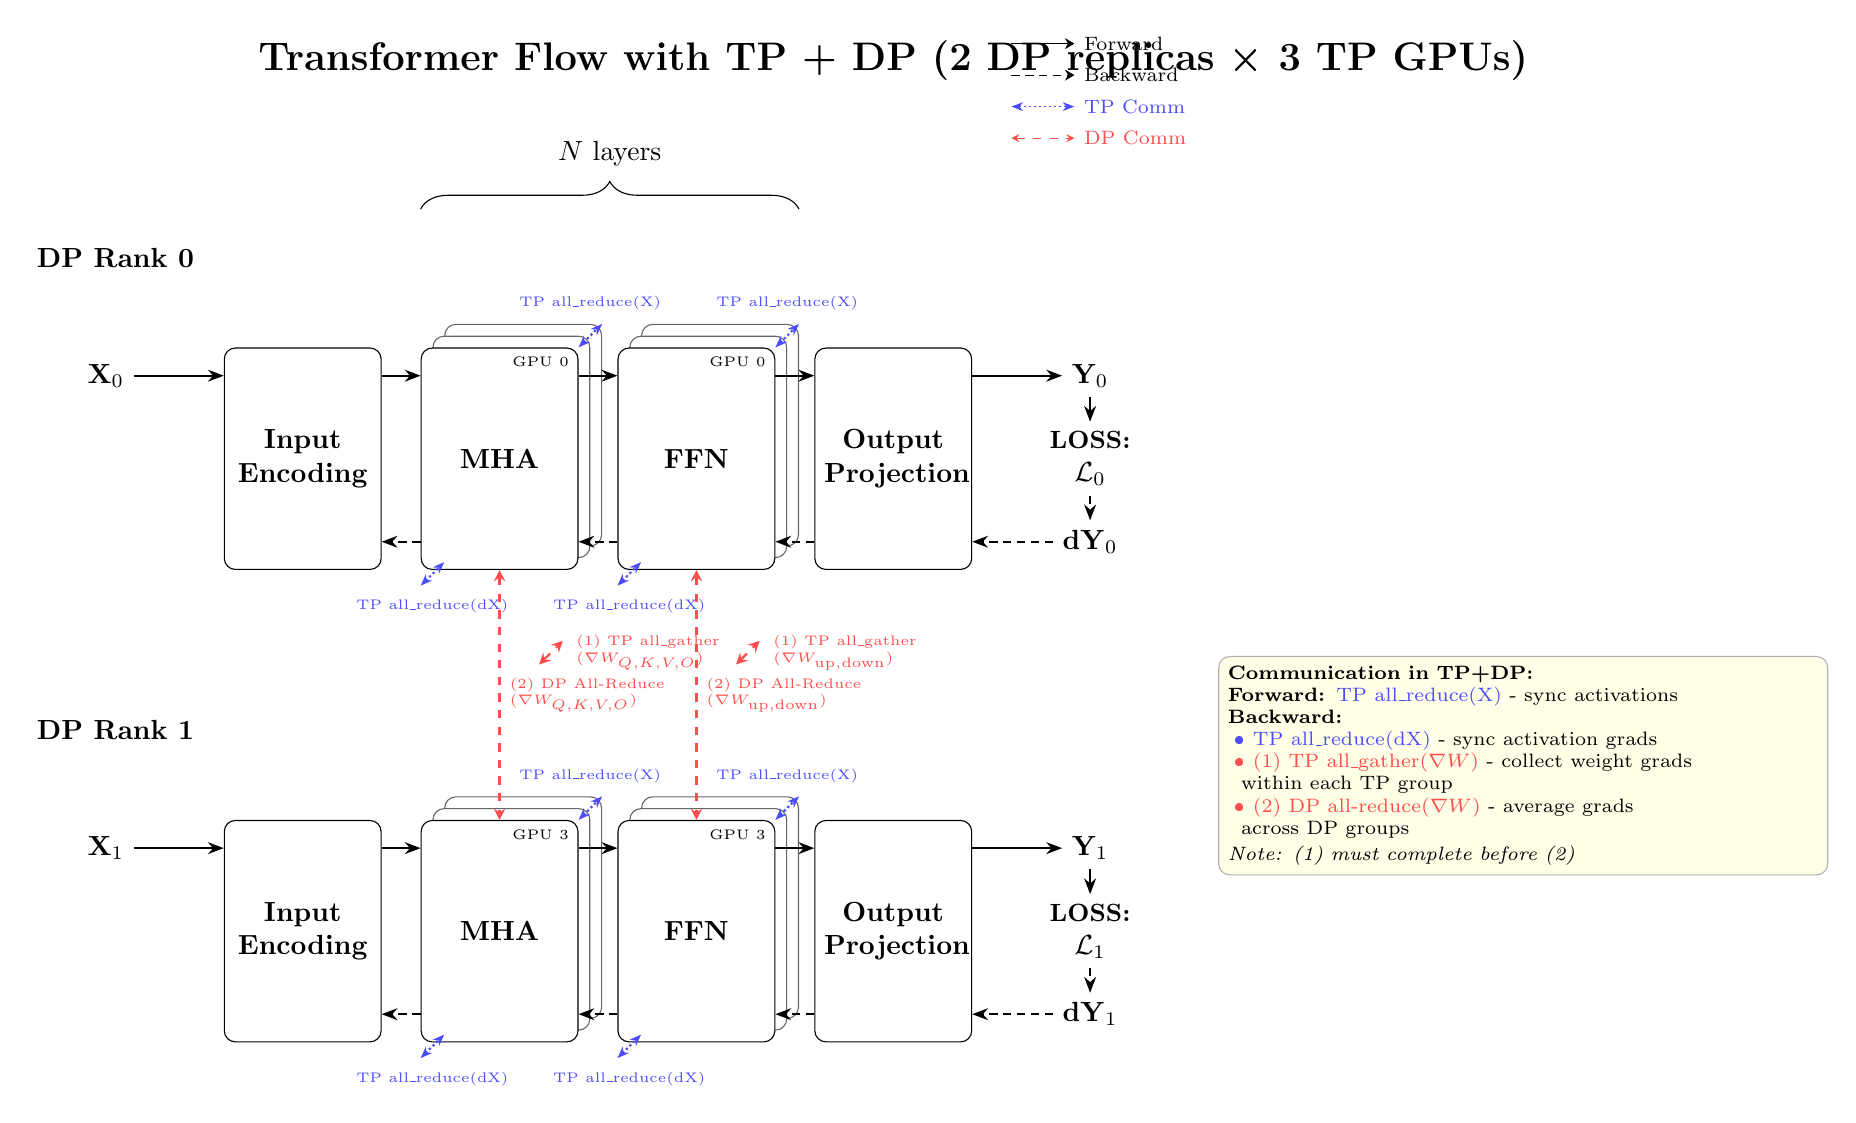
\begin{tikzpicture}[
    node distance=2.5cm,
    >=stealth,
    block/.style={rectangle, draw=black, fill=white, text width=5em, text centered, rounded corners, minimum height=8em, font=\bfseries},
    blockstack/.style={rectangle, draw=black!60, fill=white, text width=5em, text centered, rounded corners, minimum height=8em},
    forward/.style={-{Stealth[length=2mm]}, thick, black},
    backward/.style={-{Stealth[length=2mm]}, thick, black, densely dashed},
    tpcomm/.style={{Stealth[length=1.5mm]}-{Stealth[length=1.5mm]}, thick, blue!70, densely dotted},
    dpcomm/.style={<->, thick, red!70, dashed},
    io/.style={text centered, font=\bfseries}
]
    % Title
    \node[font=\Large\bfseries] at (10, 14) {Transformer Flow with TP + DP (2 DP replicas × 3 TP GPUs)};

    % ========== DP Replica 0 (Upper) ==========
    \node[font=\normalsize\bfseries, anchor=west] at (-1, 11.5) {DP Rank 0};

    \node (input_0) [io] at (0, 10) {$\mathbf{X}_0$};
    \node (encoding_0) [block, right of=input_0, yshift=-3em] {Input\\Encoding};

    % MHA blocks (3 stacked) - TP Group 0
    \node (mha3_0) [blockstack, right of=encoding_0, xshift=0.3cm, yshift=0.3cm] {};
    \node (mha2_0) [blockstack, right of=encoding_0, xshift=0.15cm, yshift=0.15cm] {};
    \node (mha_0) [block, right of=encoding_0] {MHA};
    \node[font=\tiny, anchor=north east] at (mha_0.north east) {GPU 0};

    % FFN blocks (3 stacked) - TP Group 0
    \node (mlp3_0) [blockstack, right of=mha_0, xshift=0.3cm, yshift=0.3cm] {};
    \node (mlp2_0) [blockstack, right of=mha_0, xshift=0.15cm, yshift=0.15cm] {};
    \node (mlp_0) [block, right of=mha_0] {FFN};
    \node[font=\tiny, anchor=north east] at (mlp_0.north east) {GPU 0};

    \node (output_0) [block, right of=mlp_0] {Output\\Projection};
    \node (pred_0) [io, right of=output_0, yshift=3em] {$\mathbf{Y}_0$};
    \node (loss_0) [align=center, io, right of=output_0] {\small LOSS:\\$\mathcal{L}_0$};
    \node (gradient_0) [io, right of=output_0, yshift=-3em] {$\mathbf{dY}_0$};

    % Forward arrows - DP Rank 0
    \draw [forward] (input_0) -- ([yshift=3em]encoding_0.west);
    \draw [forward] ([yshift=3em]encoding_0.east) -- ([yshift=3em]mha_0.west);
    \draw [forward] ([yshift=3em]mha_0.east) -- ([yshift=3em]mlp_0.west);
    \draw [forward] ([yshift=3em]mlp_0.east) -- ([yshift=3em]output_0.west);
    \draw [forward] ([yshift=3em]output_0.east) -- (pred_0);
    \draw [forward] (pred_0) -- (loss_0);
    \draw [backward] (loss_0) -- (gradient_0);

    % Backward arrows - DP Rank 0
    \draw [backward] (gradient_0) -- ([yshift=-3em]output_0.east);
    \draw [backward] ([yshift=-3em]output_0.west) -- ([yshift=-3em]mlp_0.east);
    \draw [backward] ([yshift=-3em]mlp_0.west) -- ([yshift=-3em]mha_0.east);
    \draw [backward] ([yshift=-3em]mha_0.west) -- ([yshift=-3em]encoding_0.east);

    % TP Communications - DP Rank 0
    % Forward All-Reduce
    \draw [tpcomm] (mha_0.north east) -- ([xshift=0.3cm, yshift=0.3cm]mha_0.north east);
    \node[font=\tiny, blue!70, anchor=south] at ([xshift=0.15cm, yshift=0.35cm]mha_0.north east) {TP all\_reduce(X)};

    \draw [tpcomm] (mlp_0.north east) -- ([xshift=0.3cm, yshift=0.3cm]mlp_0.north east);
    \node[font=\tiny, blue!70, anchor=south] at ([xshift=0.15cm, yshift=0.35cm]mlp_0.north east) {TP all\_reduce(X)};

    % Backward All-Reduce - dX
    \draw [tpcomm] ([yshift=-0.2cm]mlp_0.south west) -- ([xshift=0.3cm, yshift=0.1cm]mlp_0.south west);
    \node[font=\tiny, blue!70, anchor=north] at ([xshift=0.15cm, yshift=-0.25cm]mlp_0.south west) {TP all\_reduce(dX)};

    \draw [tpcomm] ([yshift=-0.2cm]mha_0.south west) -- ([xshift=0.3cm, yshift=0.1cm]mha_0.south west);
    \node[font=\tiny, blue!70, anchor=north] at ([xshift=0.15cm, yshift=-0.25cm]mha_0.south west) {TP all\_reduce(dX)};

    % Backward All-Gather for gradients - positioned on right side, before DP all-reduce
    \draw [dpcomm] ([xshift=-0.5cm, yshift=-1.2cm]mlp_0.south east) -- ([xshift=-0.2cm, yshift=-0.9cm]mlp_0.south east);
    \node[font=\tiny, red!70, anchor=west, align=left] at ([xshift=-0.15cm, yshift=-1.05cm]mlp_0.south east) {(1) TP all\_gather\\$(\nabla W_{\text{up},\text{down}})$};

    \draw [dpcomm] ([xshift=-0.5cm, yshift=-1.2cm]mha_0.south east) -- ([xshift=-0.2cm, yshift=-0.9cm]mha_0.south east);
    \node[font=\tiny, red!70, anchor=west, align=left] at ([xshift=-0.15cm, yshift=-1.05cm]mha_0.south east) {(1) TP all\_gather\\$(\nabla W_{Q,K,V,O})$};

    % Brace for layer repetition - DP Rank 0
    \draw[decorate, decoration={brace, amplitude=10pt}]
        ([yshift=5.0em]mha_0.north west) -- ([xshift=0.3cm, yshift=5.0em]mlp_0.north east)
        node[midway, above=12pt, font=\normalsize] {$N$ layers};

    % ========== DP Replica 1 (Lower) ==========
    \node[font=\normalsize\bfseries, anchor=west] at (-1, 5.5) {DP Rank 1};

    \node (input_1) [io] at (0, 4) {$\mathbf{X}_1$};
    \node (encoding_1) [block, right of=input_1, yshift=-3em] {Input\\Encoding};

    % MHA blocks (3 stacked) - TP Group 1
    \node (mha3_1) [blockstack, right of=encoding_1, xshift=0.3cm, yshift=0.3cm] {};
    \node (mha2_1) [blockstack, right of=encoding_1, xshift=0.15cm, yshift=0.15cm] {};
    \node (mha_1) [block, right of=encoding_1] {MHA};
    \node[font=\tiny, anchor=north east] at (mha_1.north east) {GPU 3};

    % FFN blocks (3 stacked) - TP Group 1
    \node (mlp3_1) [blockstack, right of=mha_1, xshift=0.3cm, yshift=0.3cm] {};
    \node (mlp2_1) [blockstack, right of=mha_1, xshift=0.15cm, yshift=0.15cm] {};
    \node (mlp_1) [block, right of=mha_1] {FFN};
    \node[font=\tiny, anchor=north east] at (mlp_1.north east) {GPU 3};

    \node (output_1) [block, right of=mlp_1] {Output\\Projection};
    \node (pred_1) [io, right of=output_1, yshift=3em] {$\mathbf{Y}_1$};
    \node (loss_1) [align=center, io, right of=output_1] {\small LOSS:\\$\mathcal{L}_1$};
    \node (gradient_1) [io, right of=output_1, yshift=-3em] {$\mathbf{dY}_1$};

    % Forward arrows - DP Rank 1
    \draw [forward] (input_1) -- ([yshift=3em]encoding_1.west);
    \draw [forward] ([yshift=3em]encoding_1.east) -- ([yshift=3em]mha_1.west);
    \draw [forward] ([yshift=3em]mha_1.east) -- ([yshift=3em]mlp_1.west);
    \draw [forward] ([yshift=3em]mlp_1.east) -- ([yshift=3em]output_1.west);
    \draw [forward] ([yshift=3em]output_1.east) -- (pred_1);
    \draw [forward] (pred_1) -- (loss_1);
    \draw [backward] (loss_1) -- (gradient_1);

    % Backward arrows - DP Rank 1
    \draw [backward] (gradient_1) -- ([yshift=-3em]output_1.east);
    \draw [backward] ([yshift=-3em]output_1.west) -- ([yshift=-3em]mlp_1.east);
    \draw [backward] ([yshift=-3em]mlp_1.west) -- ([yshift=-3em]mha_1.east);
    \draw [backward] ([yshift=-3em]mha_1.west) -- ([yshift=-3em]encoding_1.east);

    % TP Communications - DP Rank 1
    % Forward All-Reduce
    \draw [tpcomm] (mha_1.north east) -- ([xshift=0.3cm, yshift=0.3cm]mha_1.north east);
    \node[font=\tiny, blue!70, anchor=south] at ([xshift=0.15cm, yshift=0.35cm]mha_1.north east) {TP all\_reduce(X)};

    \draw [tpcomm] (mlp_1.north east) -- ([xshift=0.3cm, yshift=0.3cm]mlp_1.north east);
    \node[font=\tiny, blue!70, anchor=south] at ([xshift=0.15cm, yshift=0.35cm]mlp_1.north east) {TP all\_reduce(X)};

    % Backward All-Reduce - dX
    \draw [tpcomm] ([yshift=-0.2cm]mlp_1.south west) -- ([xshift=0.3cm, yshift=0.1cm]mlp_1.south west);
    \node[font=\tiny, blue!70, anchor=north] at ([xshift=0.15cm, yshift=-0.25cm]mlp_1.south west) {TP all\_reduce(dX)};

    \draw [tpcomm] ([yshift=-0.2cm]mha_1.south west) -- ([xshift=0.3cm, yshift=0.1cm]mha_1.south west);
    \node[font=\tiny, blue!70, anchor=north] at ([xshift=0.15cm, yshift=-0.25cm]mha_1.south west) {TP all\_reduce(dX)};

    % Backward All-Gather for gradients - positioned on right side, before DP all-reduce
    % \draw [dpcomm] ([xshift=0.5cm, yshift=-1.2cm]mlp_1.south east) -- ([xshift=0.8cm, yshift=-0.9cm]mlp_1.south east);
    % \node[font=\tiny, red!70, anchor=west, align=left] at ([xshift=0.85cm, yshift=-1.05cm]mlp_1.south east) {(1) TP all\_gather\\$(\nabla W_{\text{up},\text{down}})$};

    % \draw [dpcomm] ([xshift=0.5cm, yshift=-1.2cm]mha_1.south east) -- ([xshift=0.8cm, yshift=-0.9cm]mha_1.south east);
    % \node[font=\tiny, red!70, anchor=west, align=left] at ([xshift=0.85cm, yshift=-1.05cm]mha_1.south east) {(1) TP all\_gather\\$(\nabla W_{Q,K,V,O})$};

    % ========== DP Communications (Between TP Groups) ==========
    \draw [dpcomm] (mha_0.south) -- (mha_1.north) node[midway, right, font=\tiny, align=left, red!70] {(2) DP All-Reduce\\$(\nabla W_{Q,K,V,O})$};
    \draw [dpcomm] (mlp_0.south) -- (mlp_1.north) node[midway, right, font=\tiny, align=left, red!70] {(2) DP All-Reduce\\$(\nabla W_{\text{up},\text{down}})$};

    % Communication Order Annotation
    \node[font=\scriptsize, align=left, text width=7.5cm, draw=black!30, fill=yellow!10, rounded corners] at ([xshift=15.5cm, yshift=10em]encoding_1.south) {
        \textbf{Communication in TP+DP:}\\
        \textbf{Forward:} \textcolor{blue!70}{TP all\_reduce(X)} - sync activations\\
        \textbf{Backward:}\\
        \hspace{0.3em}\textcolor{blue!70}{• TP all\_reduce(dX)} - sync activation grads\\
        \hspace{0.3em}\textcolor{red!70}{• (1) TP all\_gather($\nabla W$)} - collect weight grads\\
        \hspace{0.6em}within each TP group\\
        \hspace{0.3em}\textcolor{red!70}{• (2) DP all-reduce($\nabla W$)} - average grads\\
        \hspace{0.6em}across DP groups\\[0.2em]
        \textit{Note: (1) must complete before (2)}
    };

    % Labels (Legend)
    \coordinate (legend) at ([xshift=11.5cm, yshift=12em]input_0);

    % Forward
    \draw[forward, -{Stealth[length=1.2mm,width=1.4mm]}, line width=0.3pt] (legend) -- ++(0.8,0)
      node[right, font=\scriptsize] {Forward};

    % Backward
    \draw[backward, -{Stealth[length=1.2mm,width=1.4mm]}, line width=0.3pt] ([yshift=-0.4cm]legend) -- ++(0.8,0)
      node[right, font=\scriptsize] {Backward};

    % TP Comm
    \draw[tpcomm, line width=0.3pt] ([yshift=-0.8cm]legend) -- ++(0.8,0)
      node[right, font=\scriptsize] {TP Comm};

    % DP Comm
    \draw[dpcomm, line width=0.3pt] ([yshift=-1.2cm]legend) -- ++(0.8,0)
      node[right, font=\scriptsize] {DP Comm};

\end{tikzpicture}%
}

\clearpage

% ==========================================================
% 8. Summary and Practical Takeaways
% ==========================================================
\section{Summary and Practical Takeaways}

We summarize the main ideas:
\begin{itemize}
  \item How a Transformer layer operates as a composition of
        embedding, MHA, MLP, and output projection blocks.
  \item How tensor shapes evolve through forward and backward passes.
  \item How single-node execution extends to tensor parallelism, data
        parallelism, and their combination.
\end{itemize}

We also highlight how these diagrams can be used as a reference when
designing or debugging large-scale Transformer training and inference
systems.

\end{document}
